\documentclass[twoside]{book}

% Packages required by doxygen
\usepackage{fixltx2e}
\usepackage{calc}
\usepackage{doxygen}
\usepackage[export]{adjustbox} % also loads graphicx
\usepackage{graphicx}
\usepackage[utf8]{inputenc}
\usepackage{makeidx}
\usepackage{multicol}
\usepackage{multirow}
\PassOptionsToPackage{warn}{textcomp}
\usepackage{textcomp}
\usepackage[nointegrals]{wasysym}
\usepackage[table]{xcolor}

% Font selection
\usepackage[T1]{fontenc}
\usepackage[scaled=.90]{helvet}
\usepackage{courier}
\usepackage{amssymb}
\usepackage{sectsty}
\renewcommand{\familydefault}{\sfdefault}
\allsectionsfont{%
  \fontseries{bc}\selectfont%
  \color{darkgray}%
}
\renewcommand{\DoxyLabelFont}{%
  \fontseries{bc}\selectfont%
  \color{darkgray}%
}
\newcommand{\+}{\discretionary{\mbox{\scriptsize$\hookleftarrow$}}{}{}}

% Page & text layout
\usepackage{geometry}
\geometry{%
  a4paper,%
  top=2.5cm,%
  bottom=2.5cm,%
  left=2.5cm,%
  right=2.5cm%
}
\tolerance=750
\hfuzz=15pt
\hbadness=750
\setlength{\emergencystretch}{15pt}
\setlength{\parindent}{0cm}
\setlength{\parskip}{3ex plus 2ex minus 2ex}
\makeatletter
\renewcommand{\paragraph}{%
  \@startsection{paragraph}{4}{0ex}{-1.0ex}{1.0ex}{%
    \normalfont\normalsize\bfseries\SS@parafont%
  }%
}
\renewcommand{\subparagraph}{%
  \@startsection{subparagraph}{5}{0ex}{-1.0ex}{1.0ex}{%
    \normalfont\normalsize\bfseries\SS@subparafont%
  }%
}
\makeatother

% Headers & footers
\usepackage{fancyhdr}
\pagestyle{fancyplain}
\fancyhead[LE]{\fancyplain{}{\bfseries\thepage}}
\fancyhead[CE]{\fancyplain{}{}}
\fancyhead[RE]{\fancyplain{}{\bfseries\leftmark}}
\fancyhead[LO]{\fancyplain{}{\bfseries\rightmark}}
\fancyhead[CO]{\fancyplain{}{}}
\fancyhead[RO]{\fancyplain{}{\bfseries\thepage}}
\fancyfoot[LE]{\fancyplain{}{}}
\fancyfoot[CE]{\fancyplain{}{}}
\fancyfoot[RE]{\fancyplain{}{\bfseries\scriptsize Generated by Doxygen }}
\fancyfoot[LO]{\fancyplain{}{\bfseries\scriptsize Generated by Doxygen }}
\fancyfoot[CO]{\fancyplain{}{}}
\fancyfoot[RO]{\fancyplain{}{}}
\renewcommand{\footrulewidth}{0.4pt}
\renewcommand{\chaptermark}[1]{%
  \markboth{#1}{}%
}
\renewcommand{\sectionmark}[1]{%
  \markright{\thesection\ #1}%
}

% Indices & bibliography
\usepackage{natbib}
\usepackage[titles]{tocloft}
\setcounter{tocdepth}{3}
\setcounter{secnumdepth}{5}
\makeindex

% Hyperlinks (required, but should be loaded last)
\usepackage{ifpdf}
\ifpdf
  \usepackage[pdftex,pagebackref=true]{hyperref}
\else
  \usepackage[ps2pdf,pagebackref=true]{hyperref}
\fi
\hypersetup{%
  colorlinks=true,%
  linkcolor=blue,%
  citecolor=blue,%
  unicode%
}

% Custom commands
\newcommand{\clearemptydoublepage}{%
  \newpage{\pagestyle{empty}\cleardoublepage}%
}

\usepackage{caption}
\captionsetup{labelsep=space,justification=centering,font={bf},singlelinecheck=off,skip=4pt,position=top}

%===== C O N T E N T S =====

\begin{document}

% Titlepage & ToC
\hypersetup{pageanchor=false,
             bookmarksnumbered=true,
             pdfencoding=unicode
            }
\pagenumbering{alph}
\begin{titlepage}
\vspace*{7cm}
\begin{center}%
{\Large My Project }\\
\vspace*{1cm}
{\large Generated by Doxygen 1.8.14}\\
\end{center}
\end{titlepage}
\clearemptydoublepage
\pagenumbering{roman}
\tableofcontents
\clearemptydoublepage
\pagenumbering{arabic}
\hypersetup{pageanchor=true}

%--- Begin generated contents ---
\chapter{Hierarchical Index}
\section{Class Hierarchy}
This inheritance list is sorted roughly, but not completely, alphabetically\+:\begin{DoxyCompactList}
\item \contentsline{section}{gameboard.\+Game\+Board}{\pageref{classgameboard_1_1_game_board}}{}
\item \contentsline{section}{test.\+Game\+Board\+Test}{\pageref{classtest_1_1_game_board_test}}{}
\item \contentsline{section}{gui.\+Game.\+Game\+Position}{\pageref{enumgui_1_1_game_1_1_game_position}}{}
\item \contentsline{section}{gui.\+Game.\+Game\+Result}{\pageref{classgui_1_1_game_1_1_game_result}}{}
\item J\+Layered\+Pane\begin{DoxyCompactList}
\item \contentsline{section}{gui.\+View.\+Square\+Panel}{\pageref{classgui_1_1_view_1_1_square_panel}}{}
\end{DoxyCompactList}
\item J\+Panel\begin{DoxyCompactList}
\item \contentsline{section}{gui.\+View}{\pageref{classgui_1_1_view}}{}
\item \contentsline{section}{gui.\+View.\+Score\+Panel}{\pageref{classgui_1_1_view_1_1_score_panel}}{}
\end{DoxyCompactList}
\item \contentsline{section}{gui.\+Main}{\pageref{classgui_1_1_main}}{}
\item \contentsline{section}{pieces.\+Move}{\pageref{classpieces_1_1_move}}{}
\item \contentsline{section}{test.\+Move\+Test}{\pageref{classtest_1_1_move_test}}{}
\item \contentsline{section}{pieces.\+Piece}{\pageref{classpieces_1_1_piece}}{}
\begin{DoxyCompactList}
\item \contentsline{section}{pieces.\+Bishop}{\pageref{classpieces_1_1_bishop}}{}
\item \contentsline{section}{pieces.\+Empress}{\pageref{classpieces_1_1_empress}}{}
\item \contentsline{section}{pieces.\+Hopper}{\pageref{classpieces_1_1_hopper}}{}
\item \contentsline{section}{pieces.\+King}{\pageref{classpieces_1_1_king}}{}
\item \contentsline{section}{pieces.\+Knight}{\pageref{classpieces_1_1_knight}}{}
\item \contentsline{section}{pieces.\+Pawn}{\pageref{classpieces_1_1_pawn}}{}
\item \contentsline{section}{pieces.\+Queen}{\pageref{classpieces_1_1_queen}}{}
\item \contentsline{section}{pieces.\+Rook}{\pageref{classpieces_1_1_rook}}{}
\end{DoxyCompactList}
\item \contentsline{section}{pieces.\+Piece.\+Piece\+Color}{\pageref{enumpieces_1_1_piece_1_1_piece_color}}{}
\item \contentsline{section}{test.\+Piece\+Test}{\pageref{classtest_1_1_piece_test}}{}
\begin{DoxyCompactList}
\item \contentsline{section}{test.\+Bishop\+Test}{\pageref{classtest_1_1_bishop_test}}{}
\item \contentsline{section}{test.\+Empress\+Test}{\pageref{classtest_1_1_empress_test}}{}
\item \contentsline{section}{test.\+Hopper\+Test}{\pageref{classtest_1_1_hopper_test}}{}
\item \contentsline{section}{test.\+King\+Test}{\pageref{classtest_1_1_king_test}}{}
\item \contentsline{section}{test.\+Knight\+Test}{\pageref{classtest_1_1_knight_test}}{}
\item \contentsline{section}{test.\+Pawn\+Test}{\pageref{classtest_1_1_pawn_test}}{}
\item \contentsline{section}{test.\+Queen\+Test}{\pageref{classtest_1_1_queen_test}}{}
\item \contentsline{section}{test.\+Rook\+Test}{\pageref{classtest_1_1_rook_test}}{}
\end{DoxyCompactList}
\item \contentsline{section}{pieces.\+Piece.\+Piece\+Type}{\pageref{enumpieces_1_1_piece_1_1_piece_type}}{}
\item \contentsline{section}{players.\+Player}{\pageref{classplayers_1_1_player}}{}
\begin{DoxyCompactList}
\item \contentsline{section}{players.\+Black\+Player}{\pageref{classplayers_1_1_black_player}}{}
\item \contentsline{section}{players.\+White\+Player}{\pageref{classplayers_1_1_white_player}}{}
\end{DoxyCompactList}
\item \contentsline{section}{test.\+Player\+Test}{\pageref{classtest_1_1_player_test}}{}
\begin{DoxyCompactList}
\item \contentsline{section}{test.\+Black\+Player\+Test}{\pageref{classtest_1_1_black_player_test}}{}
\item \contentsline{section}{test.\+White\+Player\+Test}{\pageref{classtest_1_1_white_player_test}}{}
\end{DoxyCompactList}
\item \contentsline{section}{gameboard.\+Square}{\pageref{classgameboard_1_1_square}}{}
\item \contentsline{section}{test.\+Square\+Test}{\pageref{classtest_1_1_square_test}}{}
\item Action\+Listener\begin{DoxyCompactList}
\item \contentsline{section}{gui.\+Button\+Controller}{\pageref{classgui_1_1_button_controller}}{}
\end{DoxyCompactList}
\item Mouse\+Listener\begin{DoxyCompactList}
\item \contentsline{section}{gui.\+Controller}{\pageref{classgui_1_1_controller}}{}
\end{DoxyCompactList}
\item Observable\begin{DoxyCompactList}
\item \contentsline{section}{gui.\+Game}{\pageref{classgui_1_1_game}}{}
\end{DoxyCompactList}
\item Observer\begin{DoxyCompactList}
\item \contentsline{section}{gui.\+View}{\pageref{classgui_1_1_view}}{}
\end{DoxyCompactList}
\end{DoxyCompactList}

\chapter{Class Index}
\section{Class List}
Here are the classes, structs, unions and interfaces with brief descriptions\+:\begin{DoxyCompactList}
\item\contentsline{section}{\mbox{\hyperlink{classpieces_1_1_bishop}{pieces.\+Bishop}} }{\pageref{classpieces_1_1_bishop}}{}
\item\contentsline{section}{\mbox{\hyperlink{classtest_1_1_bishop_test}{test.\+Bishop\+Test}} }{\pageref{classtest_1_1_bishop_test}}{}
\item\contentsline{section}{\mbox{\hyperlink{classplayers_1_1_black_player}{players.\+Black\+Player}} }{\pageref{classplayers_1_1_black_player}}{}
\item\contentsline{section}{\mbox{\hyperlink{classtest_1_1_black_player_test}{test.\+Black\+Player\+Test}} }{\pageref{classtest_1_1_black_player_test}}{}
\item\contentsline{section}{\mbox{\hyperlink{classgui_1_1_button_controller}{gui.\+Button\+Controller}} }{\pageref{classgui_1_1_button_controller}}{}
\item\contentsline{section}{\mbox{\hyperlink{classgui_1_1_controller}{gui.\+Controller}} }{\pageref{classgui_1_1_controller}}{}
\item\contentsline{section}{\mbox{\hyperlink{classpieces_1_1_empress}{pieces.\+Empress}} }{\pageref{classpieces_1_1_empress}}{}
\item\contentsline{section}{\mbox{\hyperlink{classtest_1_1_empress_test}{test.\+Empress\+Test}} }{\pageref{classtest_1_1_empress_test}}{}
\item\contentsline{section}{\mbox{\hyperlink{classgui_1_1_game}{gui.\+Game}} }{\pageref{classgui_1_1_game}}{}
\item\contentsline{section}{\mbox{\hyperlink{classgameboard_1_1_game_board}{gameboard.\+Game\+Board}} }{\pageref{classgameboard_1_1_game_board}}{}
\item\contentsline{section}{\mbox{\hyperlink{classtest_1_1_game_board_test}{test.\+Game\+Board\+Test}} }{\pageref{classtest_1_1_game_board_test}}{}
\item\contentsline{section}{\mbox{\hyperlink{enumgui_1_1_game_1_1_game_position}{gui.\+Game.\+Game\+Position}} }{\pageref{enumgui_1_1_game_1_1_game_position}}{}
\item\contentsline{section}{\mbox{\hyperlink{classgui_1_1_game_1_1_game_result}{gui.\+Game.\+Game\+Result}} }{\pageref{classgui_1_1_game_1_1_game_result}}{}
\item\contentsline{section}{\mbox{\hyperlink{classpieces_1_1_hopper}{pieces.\+Hopper}} }{\pageref{classpieces_1_1_hopper}}{}
\item\contentsline{section}{\mbox{\hyperlink{classtest_1_1_hopper_test}{test.\+Hopper\+Test}} }{\pageref{classtest_1_1_hopper_test}}{}
\item\contentsline{section}{\mbox{\hyperlink{classpieces_1_1_king}{pieces.\+King}} }{\pageref{classpieces_1_1_king}}{}
\item\contentsline{section}{\mbox{\hyperlink{classtest_1_1_king_test}{test.\+King\+Test}} }{\pageref{classtest_1_1_king_test}}{}
\item\contentsline{section}{\mbox{\hyperlink{classpieces_1_1_knight}{pieces.\+Knight}} }{\pageref{classpieces_1_1_knight}}{}
\item\contentsline{section}{\mbox{\hyperlink{classtest_1_1_knight_test}{test.\+Knight\+Test}} }{\pageref{classtest_1_1_knight_test}}{}
\item\contentsline{section}{\mbox{\hyperlink{classgui_1_1_main}{gui.\+Main}} }{\pageref{classgui_1_1_main}}{}
\item\contentsline{section}{\mbox{\hyperlink{classpieces_1_1_move}{pieces.\+Move}} }{\pageref{classpieces_1_1_move}}{}
\item\contentsline{section}{\mbox{\hyperlink{classtest_1_1_move_test}{test.\+Move\+Test}} }{\pageref{classtest_1_1_move_test}}{}
\item\contentsline{section}{\mbox{\hyperlink{classpieces_1_1_pawn}{pieces.\+Pawn}} }{\pageref{classpieces_1_1_pawn}}{}
\item\contentsline{section}{\mbox{\hyperlink{classtest_1_1_pawn_test}{test.\+Pawn\+Test}} }{\pageref{classtest_1_1_pawn_test}}{}
\item\contentsline{section}{\mbox{\hyperlink{classpieces_1_1_piece}{pieces.\+Piece}} }{\pageref{classpieces_1_1_piece}}{}
\item\contentsline{section}{\mbox{\hyperlink{enumpieces_1_1_piece_1_1_piece_color}{pieces.\+Piece.\+Piece\+Color}} }{\pageref{enumpieces_1_1_piece_1_1_piece_color}}{}
\item\contentsline{section}{\mbox{\hyperlink{classtest_1_1_piece_test}{test.\+Piece\+Test}} }{\pageref{classtest_1_1_piece_test}}{}
\item\contentsline{section}{\mbox{\hyperlink{enumpieces_1_1_piece_1_1_piece_type}{pieces.\+Piece.\+Piece\+Type}} }{\pageref{enumpieces_1_1_piece_1_1_piece_type}}{}
\item\contentsline{section}{\mbox{\hyperlink{classplayers_1_1_player}{players.\+Player}} }{\pageref{classplayers_1_1_player}}{}
\item\contentsline{section}{\mbox{\hyperlink{classtest_1_1_player_test}{test.\+Player\+Test}} }{\pageref{classtest_1_1_player_test}}{}
\item\contentsline{section}{\mbox{\hyperlink{classpieces_1_1_queen}{pieces.\+Queen}} }{\pageref{classpieces_1_1_queen}}{}
\item\contentsline{section}{\mbox{\hyperlink{classtest_1_1_queen_test}{test.\+Queen\+Test}} }{\pageref{classtest_1_1_queen_test}}{}
\item\contentsline{section}{\mbox{\hyperlink{classpieces_1_1_rook}{pieces.\+Rook}} }{\pageref{classpieces_1_1_rook}}{}
\item\contentsline{section}{\mbox{\hyperlink{classtest_1_1_rook_test}{test.\+Rook\+Test}} }{\pageref{classtest_1_1_rook_test}}{}
\item\contentsline{section}{\mbox{\hyperlink{classgui_1_1_view_1_1_score_panel}{gui.\+View.\+Score\+Panel}} }{\pageref{classgui_1_1_view_1_1_score_panel}}{}
\item\contentsline{section}{\mbox{\hyperlink{classgameboard_1_1_square}{gameboard.\+Square}} }{\pageref{classgameboard_1_1_square}}{}
\item\contentsline{section}{\mbox{\hyperlink{classgui_1_1_view_1_1_square_panel}{gui.\+View.\+Square\+Panel}} }{\pageref{classgui_1_1_view_1_1_square_panel}}{}
\item\contentsline{section}{\mbox{\hyperlink{classtest_1_1_square_test}{test.\+Square\+Test}} }{\pageref{classtest_1_1_square_test}}{}
\item\contentsline{section}{\mbox{\hyperlink{classgui_1_1_view}{gui.\+View}} }{\pageref{classgui_1_1_view}}{}
\item\contentsline{section}{\mbox{\hyperlink{classplayers_1_1_white_player}{players.\+White\+Player}} }{\pageref{classplayers_1_1_white_player}}{}
\item\contentsline{section}{\mbox{\hyperlink{classtest_1_1_white_player_test}{test.\+White\+Player\+Test}} }{\pageref{classtest_1_1_white_player_test}}{}
\end{DoxyCompactList}

\chapter{Class Documentation}
\hypertarget{classpieces_1_1_bishop}{}\section{pieces.\+Bishop Class Reference}
\label{classpieces_1_1_bishop}\index{pieces.\+Bishop@{pieces.\+Bishop}}
Inheritance diagram for pieces.\+Bishop\+:\begin{figure}[H]
\begin{center}
\leavevmode
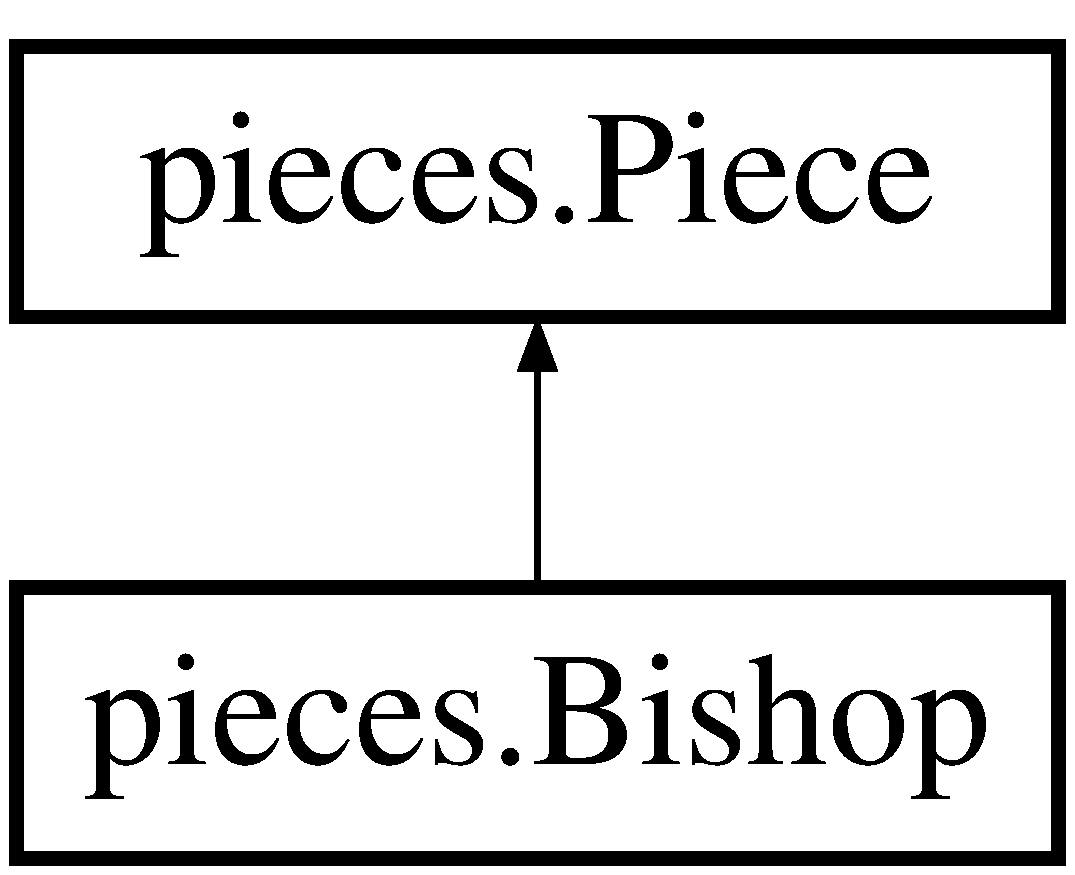
\includegraphics[height=2.000000cm]{classpieces_1_1_bishop}
\end{center}
\end{figure}
\subsection*{Public Member Functions}
\begin{DoxyCompactItemize}
\item 
\mbox{\Hypertarget{classpieces_1_1_bishop_ab1dc4c94ace53398203ed123aeb96a14}\label{classpieces_1_1_bishop_ab1dc4c94ace53398203ed123aeb96a14}} 
{\bfseries Bishop} (\mbox{\hyperlink{enumpieces_1_1_piece_1_1_piece_color}{Piece\+Color}} piece\+Color, int coordinate\+Row, int coordinate\+Col)
\item 
\mbox{\Hypertarget{classpieces_1_1_bishop_a02ba8587ac0493759c37f172a44ad20c}\label{classpieces_1_1_bishop_a02ba8587ac0493759c37f172a44ad20c}} 
List$<$ \mbox{\hyperlink{classpieces_1_1_move}{Move}} $>$ {\bfseries compute\+Valid\+Moves} (\mbox{\hyperlink{classgameboard_1_1_game_board}{Game\+Board}} board)
\item 
\mbox{\Hypertarget{classpieces_1_1_bishop_a3fdce11e2403c4d4650928214810f567}\label{classpieces_1_1_bishop_a3fdce11e2403c4d4650928214810f567}} 
String {\bfseries get\+String} ()
\end{DoxyCompactItemize}
\subsection*{Additional Inherited Members}


\subsection{Detailed Description}
Represents a \mbox{\hyperlink{classpieces_1_1_bishop}{Bishop}} piece of the chess game Created by Siyang\+Liu on 2018/2/2. 

The documentation for this class was generated from the following file\+:\begin{DoxyCompactItemize}
\item 
src/pieces/Bishop.\+java\end{DoxyCompactItemize}

\hypertarget{classtest_1_1_bishop_test}{}\section{test.\+Bishop\+Test Class Reference}
\label{classtest_1_1_bishop_test}\index{test.\+Bishop\+Test@{test.\+Bishop\+Test}}
Inheritance diagram for test.\+Bishop\+Test\+:\begin{figure}[H]
\begin{center}
\leavevmode
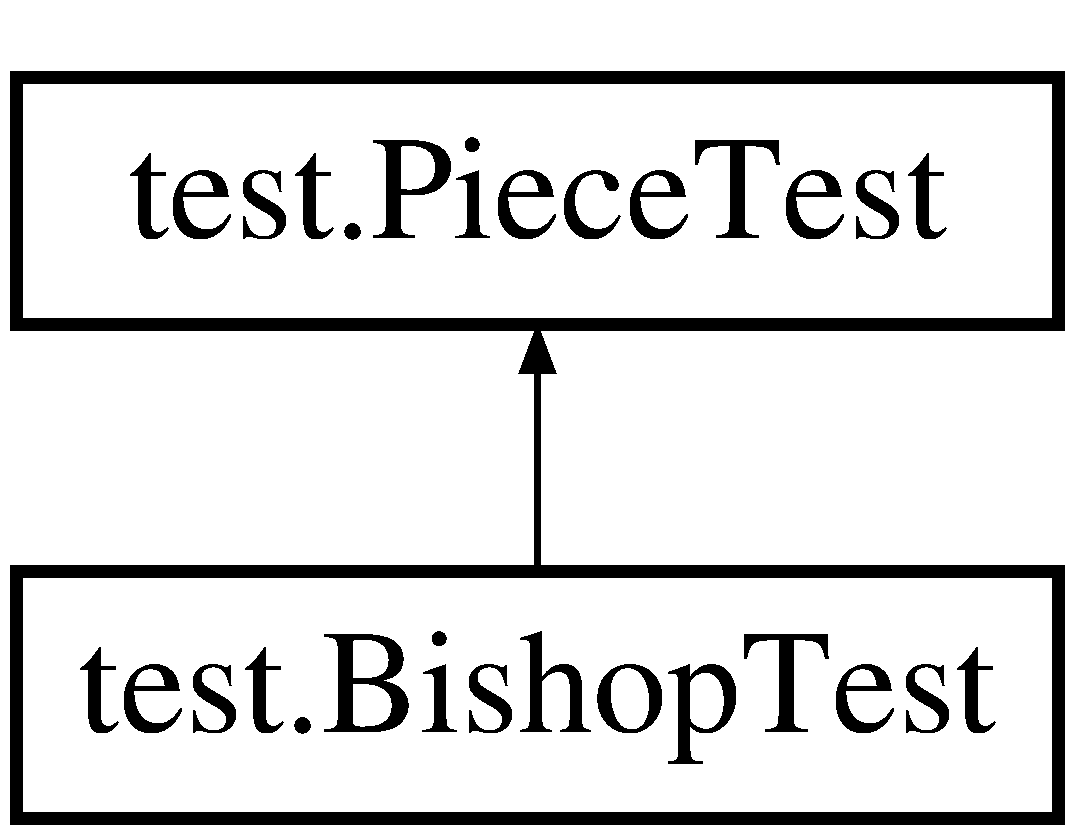
\includegraphics[height=2.000000cm]{classtest_1_1_bishop_test}
\end{center}
\end{figure}
\subsection*{Public Member Functions}
\begin{DoxyCompactItemize}
\item 
\mbox{\Hypertarget{classtest_1_1_bishop_test_afe24c52797af2017636f5b4281c9dbfa}\label{classtest_1_1_bishop_test_afe24c52797af2017636f5b4281c9dbfa}} 
void {\bfseries Valid\+Constructor2} ()  throws Exception 
\item 
\mbox{\Hypertarget{classtest_1_1_bishop_test_a105307f417e76a95ff538113c10f51ce}\label{classtest_1_1_bishop_test_a105307f417e76a95ff538113c10f51ce}} 
void {\bfseries compute\+Valid\+Moves} ()  throws Exception 
\end{DoxyCompactItemize}
\subsection*{Protected Member Functions}
\begin{DoxyCompactItemize}
\item 
\mbox{\Hypertarget{classtest_1_1_bishop_test_a60e61e7acbe7fa0265a4404f2e0f7fd2}\label{classtest_1_1_bishop_test_a60e61e7acbe7fa0265a4404f2e0f7fd2}} 
\mbox{\hyperlink{classpieces_1_1_piece}{Piece}} {\bfseries get\+Concrete} (Piece.\+Piece\+Color piece\+Color, int coordinate\+Row, int coordinate\+Col)
\end{DoxyCompactItemize}
\subsection*{Additional Inherited Members}


\subsection{Detailed Description}
Test for the operations of a Bishop Created by Siyang\+Liu on 2018/2/4. 

The documentation for this class was generated from the following file\+:\begin{DoxyCompactItemize}
\item 
src/test/Bishop\+Test.\+java\end{DoxyCompactItemize}

\hypertarget{classplayers_1_1_black_player}{}\section{players.\+Black\+Player Class Reference}
\label{classplayers_1_1_black_player}\index{players.\+Black\+Player@{players.\+Black\+Player}}
Inheritance diagram for players.\+Black\+Player\+:\begin{figure}[H]
\begin{center}
\leavevmode
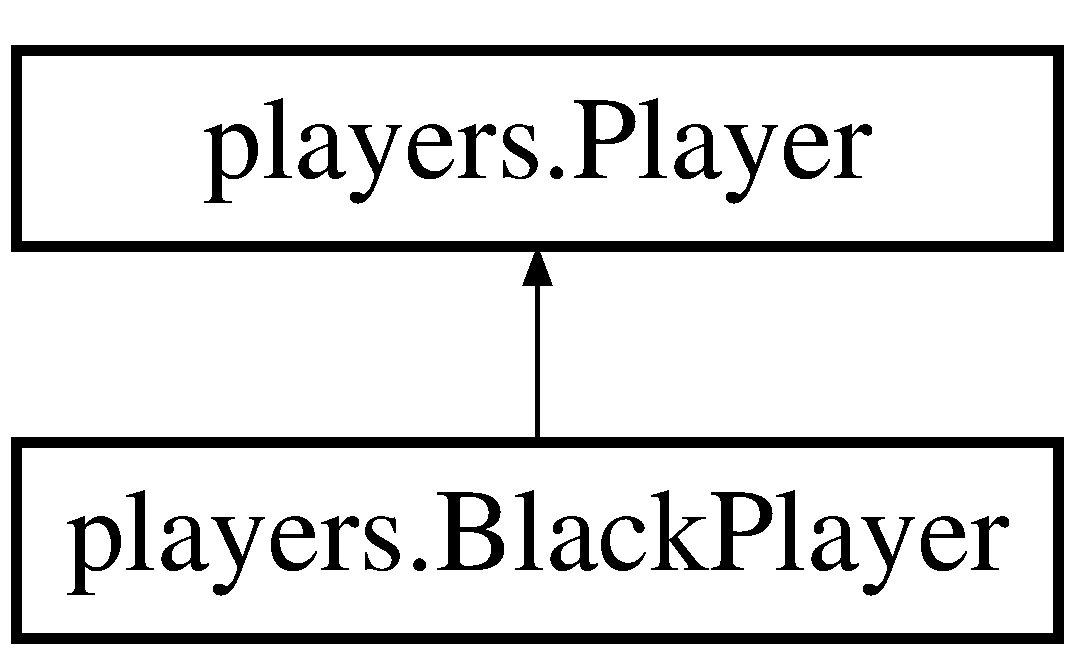
\includegraphics[height=2.000000cm]{classplayers_1_1_black_player}
\end{center}
\end{figure}
\subsection*{Public Member Functions}
\begin{DoxyCompactItemize}
\item 
\mbox{\Hypertarget{classplayers_1_1_black_player_a566125fc7169bdc81dca7ae5e84655b8}\label{classplayers_1_1_black_player_a566125fc7169bdc81dca7ae5e84655b8}} 
{\bfseries Black\+Player} (\mbox{\hyperlink{classgameboard_1_1_game_board}{Game\+Board}} board)
\item 
\mbox{\Hypertarget{classplayers_1_1_black_player_a6629df4da931d4a755313d398c87dc7b}\label{classplayers_1_1_black_player_a6629df4da931d4a755313d398c87dc7b}} 
\mbox{\hyperlink{classpieces_1_1_piece}{Piece}} {\bfseries get\+King} ()
\item 
\mbox{\Hypertarget{classplayers_1_1_black_player_acb52224c3f6bbcc9fb7f439f15c6129a}\label{classplayers_1_1_black_player_acb52224c3f6bbcc9fb7f439f15c6129a}} 
Set$<$ \mbox{\hyperlink{classpieces_1_1_piece}{Piece}} $>$ {\bfseries get\+Own\+Pieces} ()
\item 
\mbox{\Hypertarget{classplayers_1_1_black_player_ae40b8d5aad3b63fb0d3c37f8b7e39c08}\label{classplayers_1_1_black_player_ae40b8d5aad3b63fb0d3c37f8b7e39c08}} 
Set$<$ \mbox{\hyperlink{classpieces_1_1_piece}{Piece}} $>$ {\bfseries get\+Opponent\+Pieces} ()
\item 
\mbox{\Hypertarget{classplayers_1_1_black_player_afc4f0852bbb72dc9e3e194cca26616d9}\label{classplayers_1_1_black_player_afc4f0852bbb72dc9e3e194cca26616d9}} 
Piece.\+Piece\+Color {\bfseries get\+Color} ()
\end{DoxyCompactItemize}
\subsection*{Additional Inherited Members}


\subsection{Detailed Description}
Represents a player with black pieces Created by Siyang\+Liu on 2018/2/2. 

The documentation for this class was generated from the following file\+:\begin{DoxyCompactItemize}
\item 
src/players/Black\+Player.\+java\end{DoxyCompactItemize}

\hypertarget{classtest_1_1_black_player_test}{}\section{test.\+Black\+Player\+Test Class Reference}
\label{classtest_1_1_black_player_test}\index{test.\+Black\+Player\+Test@{test.\+Black\+Player\+Test}}
Inheritance diagram for test.\+Black\+Player\+Test\+:\begin{figure}[H]
\begin{center}
\leavevmode
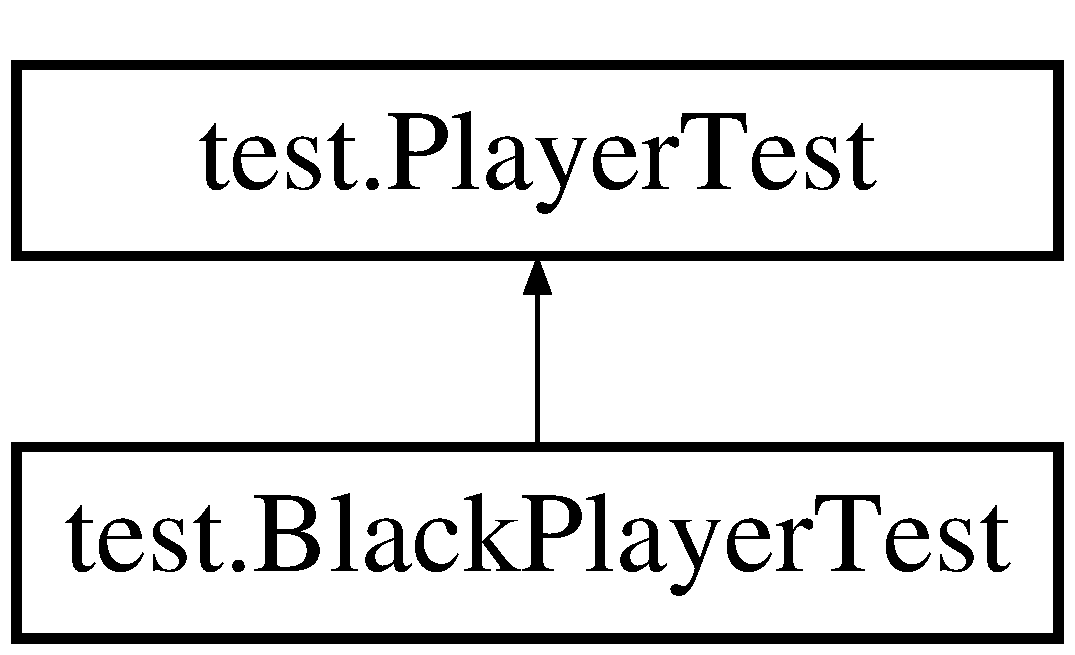
\includegraphics[height=2.000000cm]{classtest_1_1_black_player_test}
\end{center}
\end{figure}
\subsection*{Protected Member Functions}
\begin{DoxyCompactItemize}
\item 
\mbox{\Hypertarget{classtest_1_1_black_player_test_aa6c6c27aa8860f23b86b9a3ddaa44f74}\label{classtest_1_1_black_player_test_aa6c6c27aa8860f23b86b9a3ddaa44f74}} 
\mbox{\hyperlink{classplayers_1_1_player}{Player}} {\bfseries get\+Concrete\+Self} (\mbox{\hyperlink{classgameboard_1_1_game_board}{Game\+Board}} board)
\item 
\mbox{\Hypertarget{classtest_1_1_black_player_test_a9f98a8e8bc0d6acb4957c96aaae0e018}\label{classtest_1_1_black_player_test_a9f98a8e8bc0d6acb4957c96aaae0e018}} 
\mbox{\hyperlink{classplayers_1_1_player}{Player}} {\bfseries get\+Concrete\+Opponent} (\mbox{\hyperlink{classgameboard_1_1_game_board}{Game\+Board}} board)
\end{DoxyCompactItemize}
\subsection*{Additional Inherited Members}


\subsection{Detailed Description}
Test for the operations of a player with black pieces Created by Siyang\+Liu on 2018/2/4. 

The documentation for this class was generated from the following file\+:\begin{DoxyCompactItemize}
\item 
src/test/Black\+Player\+Test.\+java\end{DoxyCompactItemize}

\hypertarget{classgui_1_1_button_controller}{}\section{gui.\+Button\+Controller Class Reference}
\label{classgui_1_1_button_controller}\index{gui.\+Button\+Controller@{gui.\+Button\+Controller}}
Inheritance diagram for gui.\+Button\+Controller\+:\begin{figure}[H]
\begin{center}
\leavevmode
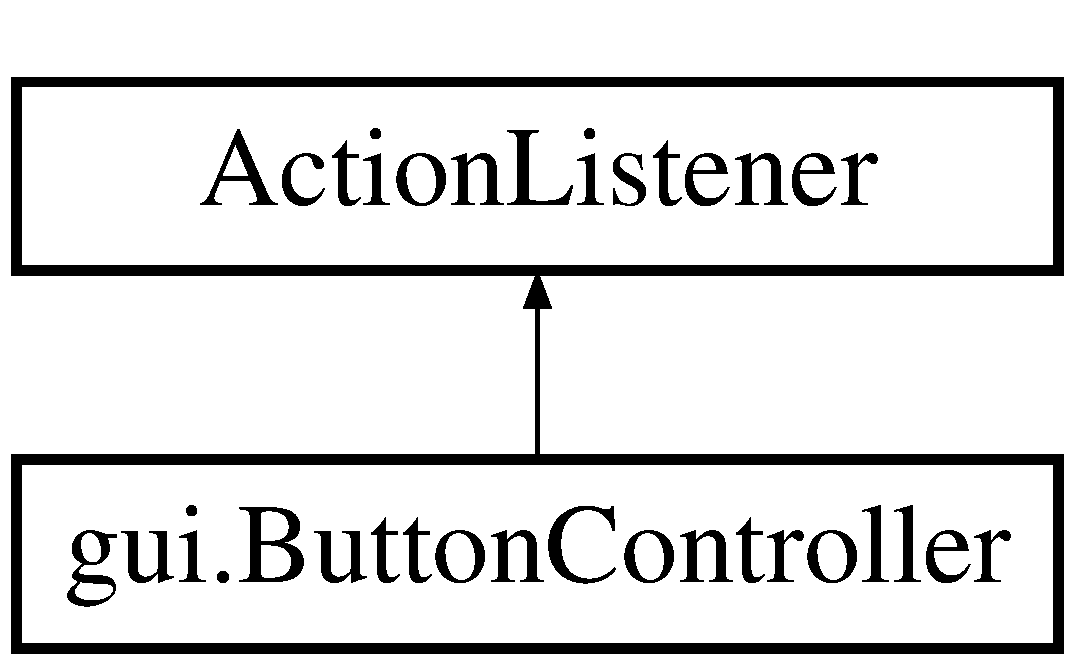
\includegraphics[height=2.000000cm]{classgui_1_1_button_controller}
\end{center}
\end{figure}
\subsection*{Public Member Functions}
\begin{DoxyCompactItemize}
\item 
\mbox{\Hypertarget{classgui_1_1_button_controller_acc997eb17fc420e45f4bf5e43b3ad1c4}\label{classgui_1_1_button_controller_acc997eb17fc420e45f4bf5e43b3ad1c4}} 
void {\bfseries action\+Performed} (Action\+Event e)
\item 
\mbox{\Hypertarget{classgui_1_1_button_controller_a074abe1c363339b11c37568609011874}\label{classgui_1_1_button_controller_a074abe1c363339b11c37568609011874}} 
void {\bfseries add\+Model} (\mbox{\hyperlink{classgui_1_1_game}{Game}} game)
\item 
\mbox{\Hypertarget{classgui_1_1_button_controller_ad924f7bcf00e53001fc0fe6c0a86ac2b}\label{classgui_1_1_button_controller_ad924f7bcf00e53001fc0fe6c0a86ac2b}} 
void {\bfseries add\+View} (\mbox{\hyperlink{classgui_1_1_view}{View}} v)
\end{DoxyCompactItemize}


\subsection{Detailed Description}
the controller of buttons and menu items in the chess game 

The documentation for this class was generated from the following file\+:\begin{DoxyCompactItemize}
\item 
src/gui/Button\+Controller.\+java\end{DoxyCompactItemize}

\hypertarget{classgui_1_1_controller}{}\section{gui.\+Controller Class Reference}
\label{classgui_1_1_controller}\index{gui.\+Controller@{gui.\+Controller}}
Inheritance diagram for gui.\+Controller\+:\begin{figure}[H]
\begin{center}
\leavevmode
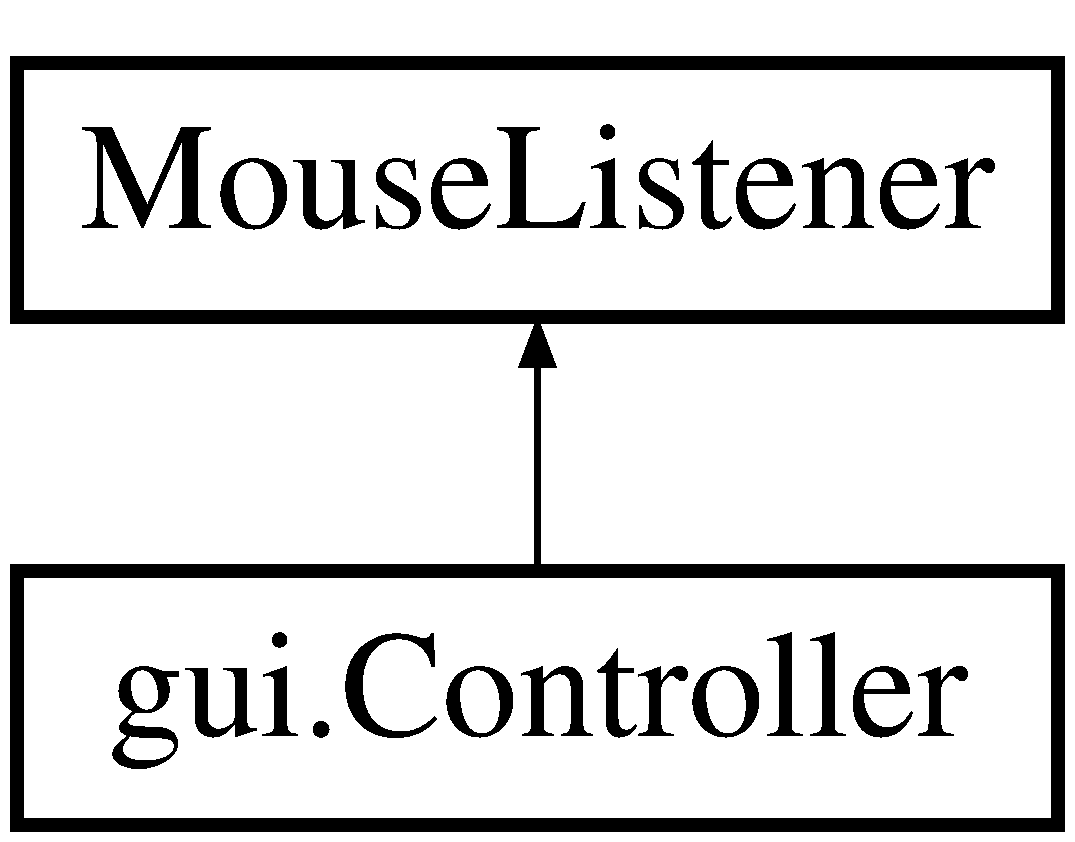
\includegraphics[height=2.000000cm]{classgui_1_1_controller}
\end{center}
\end{figure}
\subsection*{Classes}
\begin{DoxyCompactItemize}
\item 
enum {\bfseries Status}
\end{DoxyCompactItemize}
\subsection*{Public Member Functions}
\begin{DoxyCompactItemize}
\item 
void \mbox{\hyperlink{classgui_1_1_controller_a1b2b2a3f3ae423f0469883a0a67fa6d0}{add\+Model}} (\mbox{\hyperlink{classgui_1_1_game}{Game}} game)
\item 
void \mbox{\hyperlink{classgui_1_1_controller_a0bd70d2ab1480738e959182941b5acfb}{add\+View}} (\mbox{\hyperlink{classgui_1_1_view}{View}} v)
\item 
\mbox{\Hypertarget{classgui_1_1_controller_ad8cde38fdfb1d4970fa5e90de0ec6a6d}\label{classgui_1_1_controller_ad8cde38fdfb1d4970fa5e90de0ec6a6d}} 
void {\bfseries mouse\+Clicked} (Mouse\+Event e)
\item 
\mbox{\Hypertarget{classgui_1_1_controller_ab6c53d3d937195014480c6059c8662c6}\label{classgui_1_1_controller_ab6c53d3d937195014480c6059c8662c6}} 
void {\bfseries mouse\+Pressed} (Mouse\+Event e)
\item 
\mbox{\Hypertarget{classgui_1_1_controller_a55253c9f746f7389d60ad945c872f6c7}\label{classgui_1_1_controller_a55253c9f746f7389d60ad945c872f6c7}} 
void {\bfseries mouse\+Released} (Mouse\+Event e)
\item 
\mbox{\Hypertarget{classgui_1_1_controller_a860ac5f664f72e3e9897ff4e2332d1b7}\label{classgui_1_1_controller_a860ac5f664f72e3e9897ff4e2332d1b7}} 
void {\bfseries mouse\+Entered} (Mouse\+Event e)
\item 
\mbox{\Hypertarget{classgui_1_1_controller_a6399d66d0d86fbcf38734f448331c251}\label{classgui_1_1_controller_a6399d66d0d86fbcf38734f448331c251}} 
void {\bfseries mouse\+Exited} (Mouse\+Event e)
\end{DoxyCompactItemize}


\subsection{Member Function Documentation}
\mbox{\Hypertarget{classgui_1_1_controller_a1b2b2a3f3ae423f0469883a0a67fa6d0}\label{classgui_1_1_controller_a1b2b2a3f3ae423f0469883a0a67fa6d0}} 
\index{gui\+::\+Controller@{gui\+::\+Controller}!add\+Model@{add\+Model}}
\index{add\+Model@{add\+Model}!gui\+::\+Controller@{gui\+::\+Controller}}
\subsubsection{\texorpdfstring{add\+Model()}{addModel()}}
{\footnotesize\ttfamily void gui.\+Controller.\+add\+Model (\begin{DoxyParamCaption}\item[{\mbox{\hyperlink{classgui_1_1_game}{Game}}}]{game }\end{DoxyParamCaption})}

add the model to this controller 
\begin{DoxyParams}{Parameters}
{\em game} & \\
\hline
\end{DoxyParams}
\mbox{\Hypertarget{classgui_1_1_controller_a0bd70d2ab1480738e959182941b5acfb}\label{classgui_1_1_controller_a0bd70d2ab1480738e959182941b5acfb}} 
\index{gui\+::\+Controller@{gui\+::\+Controller}!add\+View@{add\+View}}
\index{add\+View@{add\+View}!gui\+::\+Controller@{gui\+::\+Controller}}
\subsubsection{\texorpdfstring{add\+View()}{addView()}}
{\footnotesize\ttfamily void gui.\+Controller.\+add\+View (\begin{DoxyParamCaption}\item[{\mbox{\hyperlink{classgui_1_1_view}{View}}}]{v }\end{DoxyParamCaption})}

add the view to this controller 
\begin{DoxyParams}{Parameters}
{\em v} & \\
\hline
\end{DoxyParams}


The documentation for this class was generated from the following file\+:\begin{DoxyCompactItemize}
\item 
src/gui/Controller.\+java\end{DoxyCompactItemize}

\hypertarget{classpieces_1_1_empress}{}\section{pieces.\+Empress Class Reference}
\label{classpieces_1_1_empress}\index{pieces.\+Empress@{pieces.\+Empress}}
Inheritance diagram for pieces.\+Empress\+:\begin{figure}[H]
\begin{center}
\leavevmode
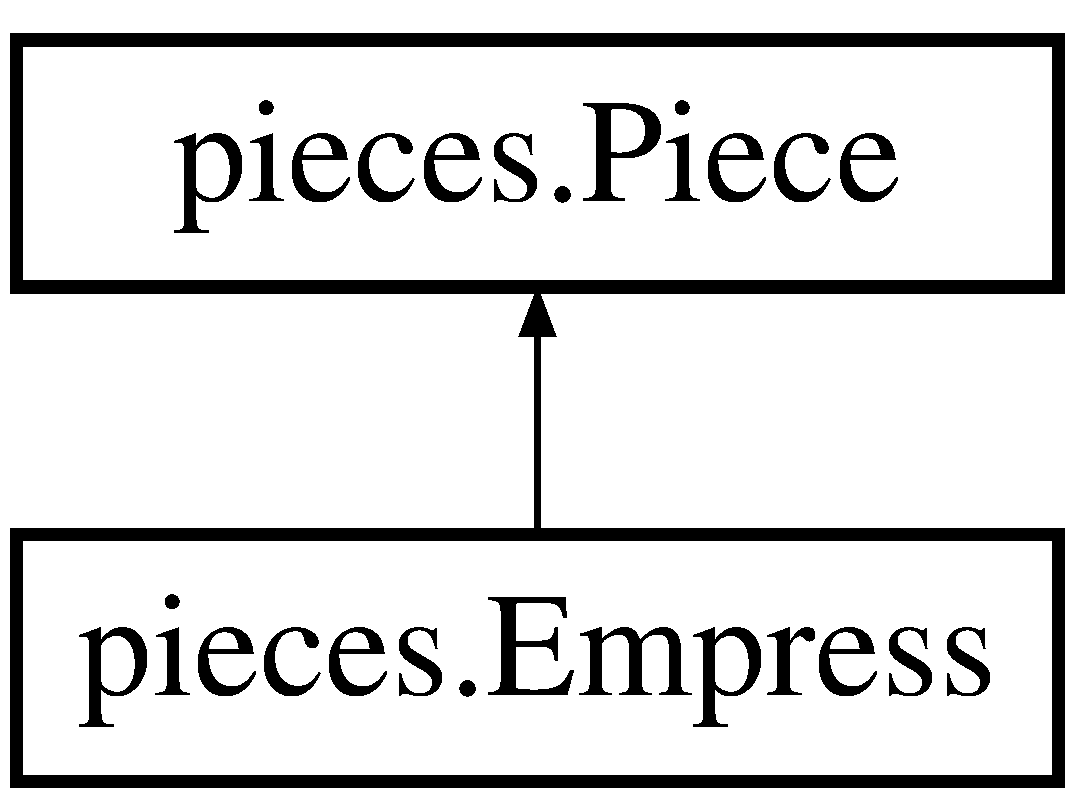
\includegraphics[height=2.000000cm]{classpieces_1_1_empress}
\end{center}
\end{figure}
\subsection*{Public Member Functions}
\begin{DoxyCompactItemize}
\item 
\mbox{\Hypertarget{classpieces_1_1_empress_a9482176b701a120d10b05d6d06c12102}\label{classpieces_1_1_empress_a9482176b701a120d10b05d6d06c12102}} 
{\bfseries Empress} (\mbox{\hyperlink{enumpieces_1_1_piece_1_1_piece_color}{Piece\+Color}} piece\+Color, int row\+Index, int col\+Index)
\item 
\mbox{\Hypertarget{classpieces_1_1_empress_a95061ef2f7ef2262f49a56e9af536509}\label{classpieces_1_1_empress_a95061ef2f7ef2262f49a56e9af536509}} 
List$<$ \mbox{\hyperlink{classpieces_1_1_move}{Move}} $>$ {\bfseries compute\+Valid\+Moves} (\mbox{\hyperlink{classgameboard_1_1_game_board}{Game\+Board}} board)
\item 
\mbox{\Hypertarget{classpieces_1_1_empress_a53a67ce2a10d71075587af667189b84f}\label{classpieces_1_1_empress_a53a67ce2a10d71075587af667189b84f}} 
String {\bfseries get\+String} ()
\end{DoxyCompactItemize}
\subsection*{Additional Inherited Members}


\subsection{Detailed Description}
An empress is a fairy chess piece that can move like a rook or a knight. 

The documentation for this class was generated from the following file\+:\begin{DoxyCompactItemize}
\item 
src/pieces/Empress.\+java\end{DoxyCompactItemize}

\hypertarget{classtest_1_1_empress_test}{}\section{test.\+Empress\+Test Class Reference}
\label{classtest_1_1_empress_test}\index{test.\+Empress\+Test@{test.\+Empress\+Test}}
Inheritance diagram for test.\+Empress\+Test\+:\begin{figure}[H]
\begin{center}
\leavevmode
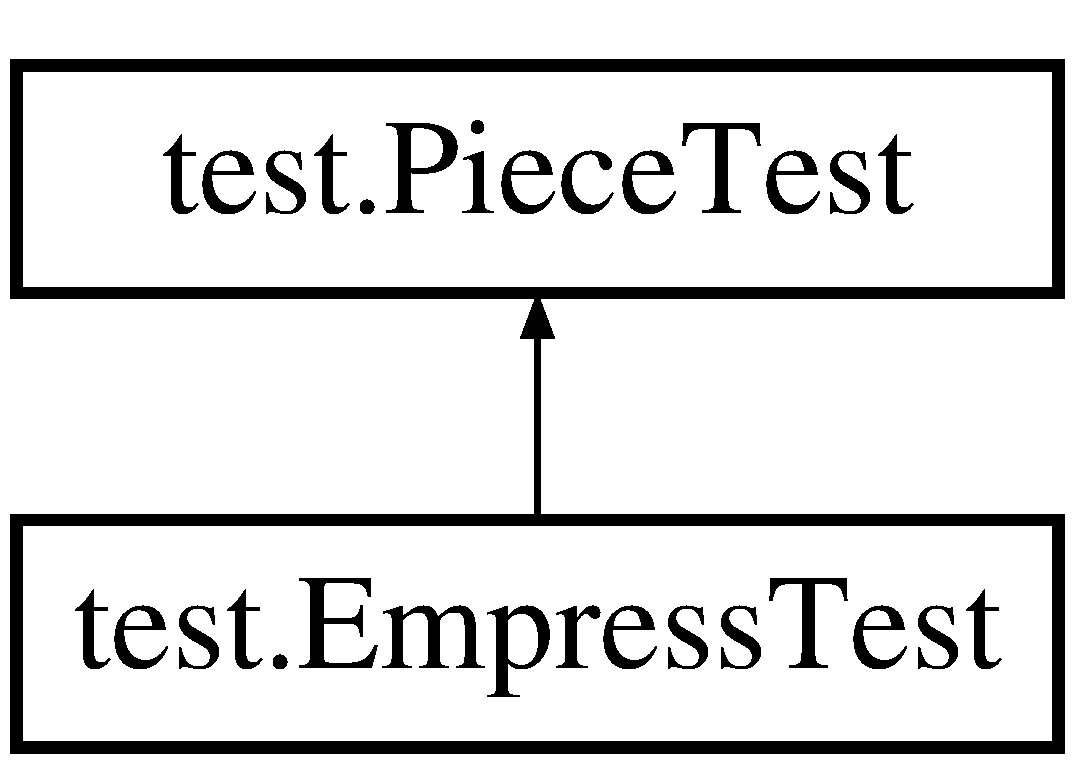
\includegraphics[height=2.000000cm]{classtest_1_1_empress_test}
\end{center}
\end{figure}
\subsection*{Public Member Functions}
\begin{DoxyCompactItemize}
\item 
\mbox{\Hypertarget{classtest_1_1_empress_test_aab262604daa5aab45f3134cc4e4319c4}\label{classtest_1_1_empress_test_aab262604daa5aab45f3134cc4e4319c4}} 
void {\bfseries Valid\+Constructor2} ()  throws Exception 
\item 
\mbox{\Hypertarget{classtest_1_1_empress_test_ad942fad7fec2c8b1911835e92f10cf4e}\label{classtest_1_1_empress_test_ad942fad7fec2c8b1911835e92f10cf4e}} 
void {\bfseries compute\+Valid\+Moves} ()  throws Exception 
\end{DoxyCompactItemize}
\subsection*{Protected Member Functions}
\begin{DoxyCompactItemize}
\item 
\mbox{\Hypertarget{classtest_1_1_empress_test_a5ad45102deaff8cfcbf90127ad8fb5ab}\label{classtest_1_1_empress_test_a5ad45102deaff8cfcbf90127ad8fb5ab}} 
\mbox{\hyperlink{classpieces_1_1_piece}{Piece}} {\bfseries get\+Concrete} (\mbox{\hyperlink{enumpieces_1_1_piece_1_1_piece_color}{Piece.\+Piece\+Color}} piece\+Color, int coordinate\+Row, int coordinate\+Col)
\end{DoxyCompactItemize}
\subsection*{Additional Inherited Members}


The documentation for this class was generated from the following file\+:\begin{DoxyCompactItemize}
\item 
src/test/Empress\+Test.\+java\end{DoxyCompactItemize}

\hypertarget{classgui_1_1_game}{}\section{gui.\+Game Class Reference}
\label{classgui_1_1_game}\index{gui.\+Game@{gui.\+Game}}
Inheritance diagram for gui.\+Game\+:\begin{figure}[H]
\begin{center}
\leavevmode
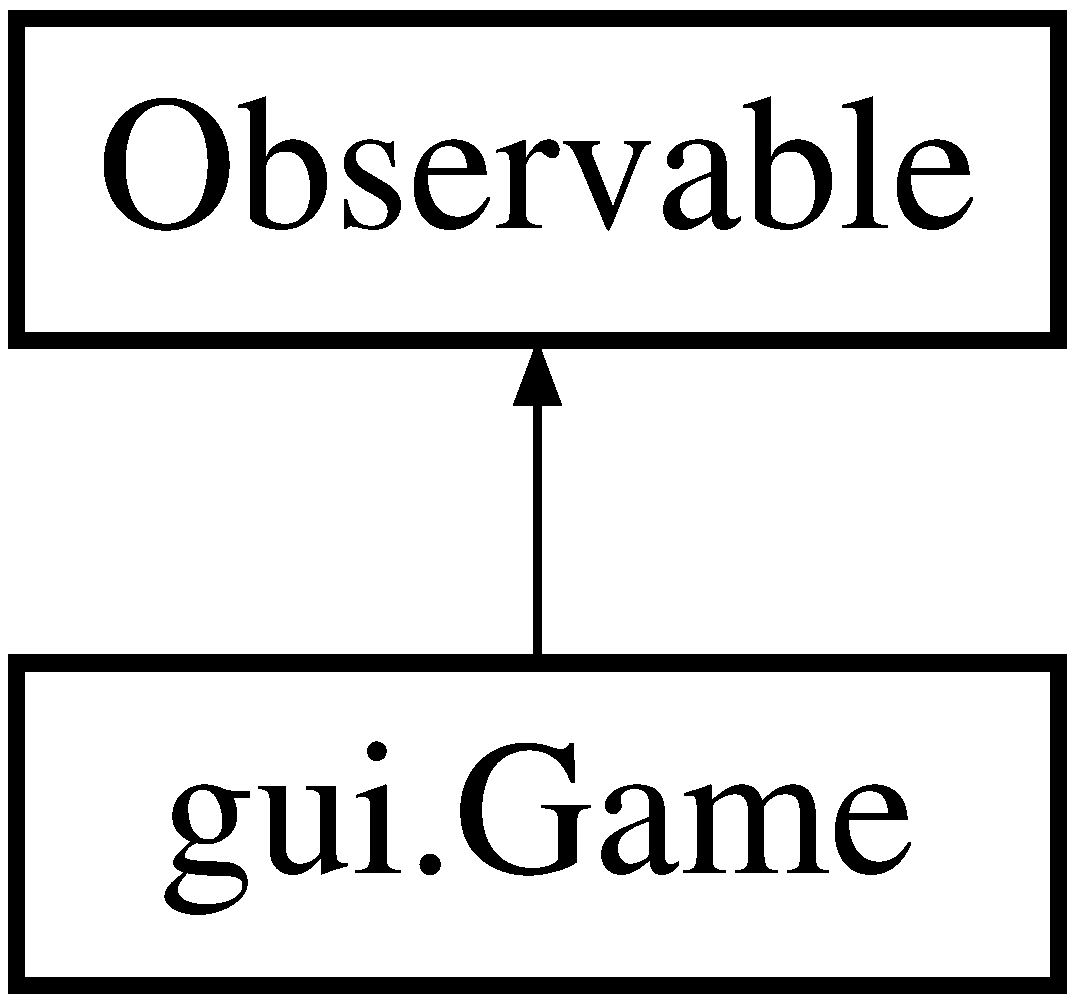
\includegraphics[height=2.000000cm]{classgui_1_1_game}
\end{center}
\end{figure}
\subsection*{Classes}
\begin{DoxyCompactItemize}
\item 
enum \mbox{\hyperlink{enumgui_1_1_game_1_1_game_position}{Game\+Position}}
\item 
class \mbox{\hyperlink{classgui_1_1_game_1_1_game_result}{Game\+Result}}
\end{DoxyCompactItemize}
\subsection*{Public Member Functions}
\begin{DoxyCompactItemize}
\item 
\mbox{\Hypertarget{classgui_1_1_game_a254e8cb4da933dad9ae00a300f07a1a4}\label{classgui_1_1_game_a254e8cb4da933dad9ae00a300f07a1a4}} 
{\bfseries Game} (int num\+Of\+Rows, int num\+Of\+Cols)
\item 
boolean \mbox{\hyperlink{classgui_1_1_game_a2ad737de5ea0e5ad722f8519ff771617}{process}} (int\mbox{[}$\,$\mbox{]} start, int\mbox{[}$\,$\mbox{]} dest)
\item 
void \mbox{\hyperlink{classgui_1_1_game_acde5ae47d364b6bddfc9be9fc535b8cc}{init\+Standard\+Game}} ()
\item 
void \mbox{\hyperlink{classgui_1_1_game_a74895d53bf09abcd355009defffb4303}{init\+Custom\+Game}} ()
\item 
boolean \mbox{\hyperlink{classgui_1_1_game_a451d11ef3789be8a74aae464c1fbfef3}{white\+Turn}} (\mbox{\hyperlink{classpieces_1_1_move}{Move}} move)
\item 
boolean \mbox{\hyperlink{classgui_1_1_game_a9f59968c4a6041a7e18a2898122a0f73}{black\+Turn}} (\mbox{\hyperlink{classpieces_1_1_move}{Move}} move)
\item 
void \mbox{\hyperlink{classgui_1_1_game_ae988eca0ead138d87285ea93d870385d}{undo}} ()
\item 
void \mbox{\hyperlink{classgui_1_1_game_a674b55155cbba7f976aa95caa017ee3b}{restart}} (boolean standard)
\item 
\mbox{\hyperlink{classgameboard_1_1_game_board}{Game\+Board}} \mbox{\hyperlink{classgui_1_1_game_afdc30ea2b00b6b06e255d3420d5c9e67}{get\+Board}} ()
\item 
\mbox{\hyperlink{classplayers_1_1_player}{Player}} \mbox{\hyperlink{classgui_1_1_game_a90a639909c028168666c3db0ac058610}{get\+White\+Player}} ()
\item 
\mbox{\hyperlink{classplayers_1_1_player}{Player}} \mbox{\hyperlink{classgui_1_1_game_a4fa4bff17684c1f215f0925e6266aeb0}{get\+Black\+Player}} ()
\item 
\mbox{\hyperlink{enumpieces_1_1_piece_1_1_piece_color}{Piece\+Color}} \mbox{\hyperlink{classgui_1_1_game_a7e5a9526328a3098b37bd3ea32f8359f}{get\+Current\+Turn}} ()
\end{DoxyCompactItemize}


\subsection{Detailed Description}
Created by Siyang\+Liu on 2018/2/2. Represents a chess game 

\subsection{Member Function Documentation}
\mbox{\Hypertarget{classgui_1_1_game_a9f59968c4a6041a7e18a2898122a0f73}\label{classgui_1_1_game_a9f59968c4a6041a7e18a2898122a0f73}} 
\index{gui\+::\+Game@{gui\+::\+Game}!black\+Turn@{black\+Turn}}
\index{black\+Turn@{black\+Turn}!gui\+::\+Game@{gui\+::\+Game}}
\subsubsection{\texorpdfstring{black\+Turn()}{blackTurn()}}
{\footnotesize\ttfamily boolean gui.\+Game.\+black\+Turn (\begin{DoxyParamCaption}\item[{\mbox{\hyperlink{classpieces_1_1_move}{Move}}}]{move }\end{DoxyParamCaption})}

let black player to move \mbox{\Hypertarget{classgui_1_1_game_a4fa4bff17684c1f215f0925e6266aeb0}\label{classgui_1_1_game_a4fa4bff17684c1f215f0925e6266aeb0}} 
\index{gui\+::\+Game@{gui\+::\+Game}!get\+Black\+Player@{get\+Black\+Player}}
\index{get\+Black\+Player@{get\+Black\+Player}!gui\+::\+Game@{gui\+::\+Game}}
\subsubsection{\texorpdfstring{get\+Black\+Player()}{getBlackPlayer()}}
{\footnotesize\ttfamily \mbox{\hyperlink{classplayers_1_1_player}{Player}} gui.\+Game.\+get\+Black\+Player (\begin{DoxyParamCaption}{ }\end{DoxyParamCaption})}

gets the black player of the game \mbox{\Hypertarget{classgui_1_1_game_afdc30ea2b00b6b06e255d3420d5c9e67}\label{classgui_1_1_game_afdc30ea2b00b6b06e255d3420d5c9e67}} 
\index{gui\+::\+Game@{gui\+::\+Game}!get\+Board@{get\+Board}}
\index{get\+Board@{get\+Board}!gui\+::\+Game@{gui\+::\+Game}}
\subsubsection{\texorpdfstring{get\+Board()}{getBoard()}}
{\footnotesize\ttfamily \mbox{\hyperlink{classgameboard_1_1_game_board}{Game\+Board}} gui.\+Game.\+get\+Board (\begin{DoxyParamCaption}{ }\end{DoxyParamCaption})}

gets the board of the game \mbox{\Hypertarget{classgui_1_1_game_a7e5a9526328a3098b37bd3ea32f8359f}\label{classgui_1_1_game_a7e5a9526328a3098b37bd3ea32f8359f}} 
\index{gui\+::\+Game@{gui\+::\+Game}!get\+Current\+Turn@{get\+Current\+Turn}}
\index{get\+Current\+Turn@{get\+Current\+Turn}!gui\+::\+Game@{gui\+::\+Game}}
\subsubsection{\texorpdfstring{get\+Current\+Turn()}{getCurrentTurn()}}
{\footnotesize\ttfamily \mbox{\hyperlink{enumpieces_1_1_piece_1_1_piece_color}{Piece\+Color}} gui.\+Game.\+get\+Current\+Turn (\begin{DoxyParamCaption}{ }\end{DoxyParamCaption})}

gets the current turn of the game \mbox{\Hypertarget{classgui_1_1_game_a90a639909c028168666c3db0ac058610}\label{classgui_1_1_game_a90a639909c028168666c3db0ac058610}} 
\index{gui\+::\+Game@{gui\+::\+Game}!get\+White\+Player@{get\+White\+Player}}
\index{get\+White\+Player@{get\+White\+Player}!gui\+::\+Game@{gui\+::\+Game}}
\subsubsection{\texorpdfstring{get\+White\+Player()}{getWhitePlayer()}}
{\footnotesize\ttfamily \mbox{\hyperlink{classplayers_1_1_player}{Player}} gui.\+Game.\+get\+White\+Player (\begin{DoxyParamCaption}{ }\end{DoxyParamCaption})}

gets the white player of the game \mbox{\Hypertarget{classgui_1_1_game_a74895d53bf09abcd355009defffb4303}\label{classgui_1_1_game_a74895d53bf09abcd355009defffb4303}} 
\index{gui\+::\+Game@{gui\+::\+Game}!init\+Custom\+Game@{init\+Custom\+Game}}
\index{init\+Custom\+Game@{init\+Custom\+Game}!gui\+::\+Game@{gui\+::\+Game}}
\subsubsection{\texorpdfstring{init\+Custom\+Game()}{initCustomGame()}}
{\footnotesize\ttfamily void gui.\+Game.\+init\+Custom\+Game (\begin{DoxyParamCaption}{ }\end{DoxyParamCaption})}

Initialize the game board with custom chess pieces \mbox{\Hypertarget{classgui_1_1_game_acde5ae47d364b6bddfc9be9fc535b8cc}\label{classgui_1_1_game_acde5ae47d364b6bddfc9be9fc535b8cc}} 
\index{gui\+::\+Game@{gui\+::\+Game}!init\+Standard\+Game@{init\+Standard\+Game}}
\index{init\+Standard\+Game@{init\+Standard\+Game}!gui\+::\+Game@{gui\+::\+Game}}
\subsubsection{\texorpdfstring{init\+Standard\+Game()}{initStandardGame()}}
{\footnotesize\ttfamily void gui.\+Game.\+init\+Standard\+Game (\begin{DoxyParamCaption}{ }\end{DoxyParamCaption})}

Initialize the game board with standard chess pieces \mbox{\Hypertarget{classgui_1_1_game_a2ad737de5ea0e5ad722f8519ff771617}\label{classgui_1_1_game_a2ad737de5ea0e5ad722f8519ff771617}} 
\index{gui\+::\+Game@{gui\+::\+Game}!process@{process}}
\index{process@{process}!gui\+::\+Game@{gui\+::\+Game}}
\subsubsection{\texorpdfstring{process()}{process()}}
{\footnotesize\ttfamily boolean gui.\+Game.\+process (\begin{DoxyParamCaption}\item[{int \mbox{[}$\,$\mbox{]}}]{start,  }\item[{int \mbox{[}$\,$\mbox{]}}]{dest }\end{DoxyParamCaption})}

Process the move from start to dest \begin{DoxyReturn}{Returns}
whether the move is legal 
\end{DoxyReturn}
\mbox{\Hypertarget{classgui_1_1_game_a674b55155cbba7f976aa95caa017ee3b}\label{classgui_1_1_game_a674b55155cbba7f976aa95caa017ee3b}} 
\index{gui\+::\+Game@{gui\+::\+Game}!restart@{restart}}
\index{restart@{restart}!gui\+::\+Game@{gui\+::\+Game}}
\subsubsection{\texorpdfstring{restart()}{restart()}}
{\footnotesize\ttfamily void gui.\+Game.\+restart (\begin{DoxyParamCaption}\item[{boolean}]{standard }\end{DoxyParamCaption})}

Restart the game 
\begin{DoxyParams}{Parameters}
{\em standard} & whether to start a standard game \\
\hline
\end{DoxyParams}
\mbox{\Hypertarget{classgui_1_1_game_ae988eca0ead138d87285ea93d870385d}\label{classgui_1_1_game_ae988eca0ead138d87285ea93d870385d}} 
\index{gui\+::\+Game@{gui\+::\+Game}!undo@{undo}}
\index{undo@{undo}!gui\+::\+Game@{gui\+::\+Game}}
\subsubsection{\texorpdfstring{undo()}{undo()}}
{\footnotesize\ttfamily void gui.\+Game.\+undo (\begin{DoxyParamCaption}{ }\end{DoxyParamCaption})}

Undo the last move executed \mbox{\Hypertarget{classgui_1_1_game_a451d11ef3789be8a74aae464c1fbfef3}\label{classgui_1_1_game_a451d11ef3789be8a74aae464c1fbfef3}} 
\index{gui\+::\+Game@{gui\+::\+Game}!white\+Turn@{white\+Turn}}
\index{white\+Turn@{white\+Turn}!gui\+::\+Game@{gui\+::\+Game}}
\subsubsection{\texorpdfstring{white\+Turn()}{whiteTurn()}}
{\footnotesize\ttfamily boolean gui.\+Game.\+white\+Turn (\begin{DoxyParamCaption}\item[{\mbox{\hyperlink{classpieces_1_1_move}{Move}}}]{move }\end{DoxyParamCaption})}

let white player to move 

The documentation for this class was generated from the following file\+:\begin{DoxyCompactItemize}
\item 
src/gui/Game.\+java\end{DoxyCompactItemize}

\hypertarget{classgameboard_1_1_game_board}{}\section{gameboard.\+Game\+Board Class Reference}
\label{classgameboard_1_1_game_board}\index{gameboard.\+Game\+Board@{gameboard.\+Game\+Board}}
\subsection*{Public Member Functions}
\begin{DoxyCompactItemize}
\item 
\mbox{\Hypertarget{classgameboard_1_1_game_board_a2744a1969fe37986c4026beec995adec}\label{classgameboard_1_1_game_board_a2744a1969fe37986c4026beec995adec}} 
{\bfseries Game\+Board} (int num\+Of\+Rows, int num\+Of\+Cols)
\item 
void \mbox{\hyperlink{classgameboard_1_1_game_board_a6e74eee1e3ec913341e6f440064d0f80}{place\+Standard\+Pieces}} ()
\item 
void \mbox{\hyperlink{classgameboard_1_1_game_board_ae7f2394074cc527b4ed933d562f08f06}{place\+Custom\+Pieces}} ()
\item 
boolean \mbox{\hyperlink{classgameboard_1_1_game_board_aee63d4310ef2ea7cb177013eed310b40}{place\+Piece}} (\mbox{\hyperlink{classpieces_1_1_piece}{Piece}} piece)
\item 
\mbox{\hyperlink{classpieces_1_1_piece}{Piece}} \mbox{\hyperlink{classgameboard_1_1_game_board_a368adac08213b4311a2897a273acc118}{execute\+Move}} (\mbox{\hyperlink{classpieces_1_1_move}{Move}} move)
\item 
void \mbox{\hyperlink{classgameboard_1_1_game_board_a82442fc13c1a73e107851235c5cd92a2}{undo\+Move}} (\mbox{\hyperlink{classpieces_1_1_move}{Move}} move, \mbox{\hyperlink{classpieces_1_1_piece}{Piece}} captured\+Piece)
\item 
boolean \mbox{\hyperlink{classgameboard_1_1_game_board_ad7fb7cf5cb3b97770bfaf5c595c5630b}{is\+Valid\+Coordinates}} (int row\+Index, int col\+Index)
\item 
int \mbox{\hyperlink{classgameboard_1_1_game_board_a6b108da59e192efeb24937121ff160ba}{get\+Num\+Of\+Rows}} ()
\item 
int \mbox{\hyperlink{classgameboard_1_1_game_board_a049d4164c15b7a60f23b12accd0c1e15}{get\+Num\+Of\+Cols}} ()
\item 
Set$<$ \mbox{\hyperlink{classpieces_1_1_piece}{Piece}} $>$ \mbox{\hyperlink{classgameboard_1_1_game_board_a6dbc8479a689353cfde617056007b5f1}{get\+Black\+Pieces}} ()
\item 
Set$<$ \mbox{\hyperlink{classpieces_1_1_piece}{Piece}} $>$ \mbox{\hyperlink{classgameboard_1_1_game_board_a5c9d9bdb8c155fbc01c72760b33dba1e}{get\+White\+Pieces}} ()
\item 
\mbox{\hyperlink{classgameboard_1_1_square}{Square}} \mbox{[}$\,$\mbox{]}\mbox{[}$\,$\mbox{]} \mbox{\hyperlink{classgameboard_1_1_game_board_a862261920d74b60acd609bfc7d1b1bc2}{get\+Squares}} ()
\item 
\mbox{\hyperlink{classgameboard_1_1_square}{Square}} \mbox{\hyperlink{classgameboard_1_1_game_board_a9a1fa2f3221dc4705f492166ce9dd071}{get\+Square}} (int row, int col)
\end{DoxyCompactItemize}


\subsection{Detailed Description}
Represents a game board of the chess game Created by Siyang\+Liu on 2018/2/2. 

\subsection{Member Function Documentation}
\mbox{\Hypertarget{classgameboard_1_1_game_board_a368adac08213b4311a2897a273acc118}\label{classgameboard_1_1_game_board_a368adac08213b4311a2897a273acc118}} 
\index{gameboard\+::\+Game\+Board@{gameboard\+::\+Game\+Board}!execute\+Move@{execute\+Move}}
\index{execute\+Move@{execute\+Move}!gameboard\+::\+Game\+Board@{gameboard\+::\+Game\+Board}}
\subsubsection{\texorpdfstring{execute\+Move()}{executeMove()}}
{\footnotesize\ttfamily \mbox{\hyperlink{classpieces_1_1_piece}{Piece}} gameboard.\+Game\+Board.\+execute\+Move (\begin{DoxyParamCaption}\item[{\mbox{\hyperlink{classpieces_1_1_move}{Move}}}]{move }\end{DoxyParamCaption})}

Executes the given move in the board 
\begin{DoxyParams}{Parameters}
{\em move} & is Guaranteed to be a valid move \\
\hline
\end{DoxyParams}
\begin{DoxyReturn}{Returns}
the captured piece after the execution of the given move 
\end{DoxyReturn}
\mbox{\Hypertarget{classgameboard_1_1_game_board_a6dbc8479a689353cfde617056007b5f1}\label{classgameboard_1_1_game_board_a6dbc8479a689353cfde617056007b5f1}} 
\index{gameboard\+::\+Game\+Board@{gameboard\+::\+Game\+Board}!get\+Black\+Pieces@{get\+Black\+Pieces}}
\index{get\+Black\+Pieces@{get\+Black\+Pieces}!gameboard\+::\+Game\+Board@{gameboard\+::\+Game\+Board}}
\subsubsection{\texorpdfstring{get\+Black\+Pieces()}{getBlackPieces()}}
{\footnotesize\ttfamily Set$<$\mbox{\hyperlink{classpieces_1_1_piece}{Piece}}$>$ gameboard.\+Game\+Board.\+get\+Black\+Pieces (\begin{DoxyParamCaption}{ }\end{DoxyParamCaption})}

gets the black pieces of the game board \mbox{\Hypertarget{classgameboard_1_1_game_board_a049d4164c15b7a60f23b12accd0c1e15}\label{classgameboard_1_1_game_board_a049d4164c15b7a60f23b12accd0c1e15}} 
\index{gameboard\+::\+Game\+Board@{gameboard\+::\+Game\+Board}!get\+Num\+Of\+Cols@{get\+Num\+Of\+Cols}}
\index{get\+Num\+Of\+Cols@{get\+Num\+Of\+Cols}!gameboard\+::\+Game\+Board@{gameboard\+::\+Game\+Board}}
\subsubsection{\texorpdfstring{get\+Num\+Of\+Cols()}{getNumOfCols()}}
{\footnotesize\ttfamily int gameboard.\+Game\+Board.\+get\+Num\+Of\+Cols (\begin{DoxyParamCaption}{ }\end{DoxyParamCaption})}

gets the number of cols of the game board \mbox{\Hypertarget{classgameboard_1_1_game_board_a6b108da59e192efeb24937121ff160ba}\label{classgameboard_1_1_game_board_a6b108da59e192efeb24937121ff160ba}} 
\index{gameboard\+::\+Game\+Board@{gameboard\+::\+Game\+Board}!get\+Num\+Of\+Rows@{get\+Num\+Of\+Rows}}
\index{get\+Num\+Of\+Rows@{get\+Num\+Of\+Rows}!gameboard\+::\+Game\+Board@{gameboard\+::\+Game\+Board}}
\subsubsection{\texorpdfstring{get\+Num\+Of\+Rows()}{getNumOfRows()}}
{\footnotesize\ttfamily int gameboard.\+Game\+Board.\+get\+Num\+Of\+Rows (\begin{DoxyParamCaption}{ }\end{DoxyParamCaption})}

gets the number of rows of the game board \mbox{\Hypertarget{classgameboard_1_1_game_board_a9a1fa2f3221dc4705f492166ce9dd071}\label{classgameboard_1_1_game_board_a9a1fa2f3221dc4705f492166ce9dd071}} 
\index{gameboard\+::\+Game\+Board@{gameboard\+::\+Game\+Board}!get\+Square@{get\+Square}}
\index{get\+Square@{get\+Square}!gameboard\+::\+Game\+Board@{gameboard\+::\+Game\+Board}}
\subsubsection{\texorpdfstring{get\+Square()}{getSquare()}}
{\footnotesize\ttfamily \mbox{\hyperlink{classgameboard_1_1_square}{Square}} gameboard.\+Game\+Board.\+get\+Square (\begin{DoxyParamCaption}\item[{int}]{row,  }\item[{int}]{col }\end{DoxyParamCaption})}

gets the the square at the given location of the game board \mbox{\Hypertarget{classgameboard_1_1_game_board_a862261920d74b60acd609bfc7d1b1bc2}\label{classgameboard_1_1_game_board_a862261920d74b60acd609bfc7d1b1bc2}} 
\index{gameboard\+::\+Game\+Board@{gameboard\+::\+Game\+Board}!get\+Squares@{get\+Squares}}
\index{get\+Squares@{get\+Squares}!gameboard\+::\+Game\+Board@{gameboard\+::\+Game\+Board}}
\subsubsection{\texorpdfstring{get\+Squares()}{getSquares()}}
{\footnotesize\ttfamily \mbox{\hyperlink{classgameboard_1_1_square}{Square}} \mbox{[}$\,$\mbox{]}\mbox{[}$\,$\mbox{]} gameboard.\+Game\+Board.\+get\+Squares (\begin{DoxyParamCaption}{ }\end{DoxyParamCaption})}

gets the square array of the game board \mbox{\Hypertarget{classgameboard_1_1_game_board_a5c9d9bdb8c155fbc01c72760b33dba1e}\label{classgameboard_1_1_game_board_a5c9d9bdb8c155fbc01c72760b33dba1e}} 
\index{gameboard\+::\+Game\+Board@{gameboard\+::\+Game\+Board}!get\+White\+Pieces@{get\+White\+Pieces}}
\index{get\+White\+Pieces@{get\+White\+Pieces}!gameboard\+::\+Game\+Board@{gameboard\+::\+Game\+Board}}
\subsubsection{\texorpdfstring{get\+White\+Pieces()}{getWhitePieces()}}
{\footnotesize\ttfamily Set$<$\mbox{\hyperlink{classpieces_1_1_piece}{Piece}}$>$ gameboard.\+Game\+Board.\+get\+White\+Pieces (\begin{DoxyParamCaption}{ }\end{DoxyParamCaption})}

gets the white pieces of the game board \mbox{\Hypertarget{classgameboard_1_1_game_board_ad7fb7cf5cb3b97770bfaf5c595c5630b}\label{classgameboard_1_1_game_board_ad7fb7cf5cb3b97770bfaf5c595c5630b}} 
\index{gameboard\+::\+Game\+Board@{gameboard\+::\+Game\+Board}!is\+Valid\+Coordinates@{is\+Valid\+Coordinates}}
\index{is\+Valid\+Coordinates@{is\+Valid\+Coordinates}!gameboard\+::\+Game\+Board@{gameboard\+::\+Game\+Board}}
\subsubsection{\texorpdfstring{is\+Valid\+Coordinates()}{isValidCoordinates()}}
{\footnotesize\ttfamily boolean gameboard.\+Game\+Board.\+is\+Valid\+Coordinates (\begin{DoxyParamCaption}\item[{int}]{row\+Index,  }\item[{int}]{col\+Index }\end{DoxyParamCaption})}

checks if the given coordinates are valid in the board \mbox{\Hypertarget{classgameboard_1_1_game_board_ae7f2394074cc527b4ed933d562f08f06}\label{classgameboard_1_1_game_board_ae7f2394074cc527b4ed933d562f08f06}} 
\index{gameboard\+::\+Game\+Board@{gameboard\+::\+Game\+Board}!place\+Custom\+Pieces@{place\+Custom\+Pieces}}
\index{place\+Custom\+Pieces@{place\+Custom\+Pieces}!gameboard\+::\+Game\+Board@{gameboard\+::\+Game\+Board}}
\subsubsection{\texorpdfstring{place\+Custom\+Pieces()}{placeCustomPieces()}}
{\footnotesize\ttfamily void gameboard.\+Game\+Board.\+place\+Custom\+Pieces (\begin{DoxyParamCaption}{ }\end{DoxyParamCaption})}

Places the initial pieces of a standard chess game onto the board \mbox{\Hypertarget{classgameboard_1_1_game_board_aee63d4310ef2ea7cb177013eed310b40}\label{classgameboard_1_1_game_board_aee63d4310ef2ea7cb177013eed310b40}} 
\index{gameboard\+::\+Game\+Board@{gameboard\+::\+Game\+Board}!place\+Piece@{place\+Piece}}
\index{place\+Piece@{place\+Piece}!gameboard\+::\+Game\+Board@{gameboard\+::\+Game\+Board}}
\subsubsection{\texorpdfstring{place\+Piece()}{placePiece()}}
{\footnotesize\ttfamily boolean gameboard.\+Game\+Board.\+place\+Piece (\begin{DoxyParamCaption}\item[{\mbox{\hyperlink{classpieces_1_1_piece}{Piece}}}]{piece }\end{DoxyParamCaption})}

Places the given piece onto the board in specified location 
\begin{DoxyParams}{Parameters}
{\em piece} & the piece to place onto the board cannot be null \\
\hline
\end{DoxyParams}
\mbox{\Hypertarget{classgameboard_1_1_game_board_a6e74eee1e3ec913341e6f440064d0f80}\label{classgameboard_1_1_game_board_a6e74eee1e3ec913341e6f440064d0f80}} 
\index{gameboard\+::\+Game\+Board@{gameboard\+::\+Game\+Board}!place\+Standard\+Pieces@{place\+Standard\+Pieces}}
\index{place\+Standard\+Pieces@{place\+Standard\+Pieces}!gameboard\+::\+Game\+Board@{gameboard\+::\+Game\+Board}}
\subsubsection{\texorpdfstring{place\+Standard\+Pieces()}{placeStandardPieces()}}
{\footnotesize\ttfamily void gameboard.\+Game\+Board.\+place\+Standard\+Pieces (\begin{DoxyParamCaption}{ }\end{DoxyParamCaption})}

Places the initial pieces of a standard chess game onto the board \mbox{\Hypertarget{classgameboard_1_1_game_board_a82442fc13c1a73e107851235c5cd92a2}\label{classgameboard_1_1_game_board_a82442fc13c1a73e107851235c5cd92a2}} 
\index{gameboard\+::\+Game\+Board@{gameboard\+::\+Game\+Board}!undo\+Move@{undo\+Move}}
\index{undo\+Move@{undo\+Move}!gameboard\+::\+Game\+Board@{gameboard\+::\+Game\+Board}}
\subsubsection{\texorpdfstring{undo\+Move()}{undoMove()}}
{\footnotesize\ttfamily void gameboard.\+Game\+Board.\+undo\+Move (\begin{DoxyParamCaption}\item[{\mbox{\hyperlink{classpieces_1_1_move}{Move}}}]{move,  }\item[{\mbox{\hyperlink{classpieces_1_1_piece}{Piece}}}]{captured\+Piece }\end{DoxyParamCaption})}

Undoes the given move in the board 
\begin{DoxyParams}{Parameters}
{\em move} & the move to undo and was guaranteed to be a valid move \\
\hline
{\em captured\+Piece} & the piece capture after the move was executed \\
\hline
\end{DoxyParams}


The documentation for this class was generated from the following file\+:\begin{DoxyCompactItemize}
\item 
src/gameboard/Game\+Board.\+java\end{DoxyCompactItemize}

\hypertarget{classtest_1_1_game_board_test}{}\section{test.\+Game\+Board\+Test Class Reference}
\label{classtest_1_1_game_board_test}\index{test.\+Game\+Board\+Test@{test.\+Game\+Board\+Test}}
\subsection*{Public Member Functions}
\begin{DoxyCompactItemize}
\item 
\mbox{\Hypertarget{classtest_1_1_game_board_test_a57003188298acb6a4f21436c6cb7feaf}\label{classtest_1_1_game_board_test_a57003188298acb6a4f21436c6cb7feaf}} 
void {\bfseries create\+Empty\+Board\+For\+Test} ()
\item 
void \mbox{\hyperlink{classtest_1_1_game_board_test_a45e7ff57d223c2ebb209cc35f8b0d916}{Valid\+Constructor}} ()  throws Exception 
\item 
void \mbox{\hyperlink{classtest_1_1_game_board_test_ae0458820f080e86163d12ff75d019f9a}{place\+Standard\+Pieces}} ()  throws Exception 
\item 
void \mbox{\hyperlink{classtest_1_1_game_board_test_abcac1900d5c33b34015c93f1862a915f}{move\+Piece1}} ()  throws Exception 
\item 
void \mbox{\hyperlink{classtest_1_1_game_board_test_acac01404dbfc189519f2e21f4105d7e2}{move\+Piece2}} ()  throws Exception 
\end{DoxyCompactItemize}


\subsection{Detailed Description}
Created by Siyang\+Liu on 2018/2/3. 

\subsection{Member Function Documentation}
\mbox{\Hypertarget{classtest_1_1_game_board_test_abcac1900d5c33b34015c93f1862a915f}\label{classtest_1_1_game_board_test_abcac1900d5c33b34015c93f1862a915f}} 
\index{test\+::\+Game\+Board\+Test@{test\+::\+Game\+Board\+Test}!move\+Piece1@{move\+Piece1}}
\index{move\+Piece1@{move\+Piece1}!test\+::\+Game\+Board\+Test@{test\+::\+Game\+Board\+Test}}
\subsubsection{\texorpdfstring{move\+Piece1()}{movePiece1()}}
{\footnotesize\ttfamily void test.\+Game\+Board\+Test.\+move\+Piece1 (\begin{DoxyParamCaption}{ }\end{DoxyParamCaption}) throws Exception}

precondition\+: the update\+Piece\+Coordinates is valid \mbox{\Hypertarget{classtest_1_1_game_board_test_acac01404dbfc189519f2e21f4105d7e2}\label{classtest_1_1_game_board_test_acac01404dbfc189519f2e21f4105d7e2}} 
\index{test\+::\+Game\+Board\+Test@{test\+::\+Game\+Board\+Test}!move\+Piece2@{move\+Piece2}}
\index{move\+Piece2@{move\+Piece2}!test\+::\+Game\+Board\+Test@{test\+::\+Game\+Board\+Test}}
\subsubsection{\texorpdfstring{move\+Piece2()}{movePiece2()}}
{\footnotesize\ttfamily void test.\+Game\+Board\+Test.\+move\+Piece2 (\begin{DoxyParamCaption}{ }\end{DoxyParamCaption}) throws Exception}

precondition\+: the update\+Piece\+Coordinates is valid \mbox{\Hypertarget{classtest_1_1_game_board_test_ae0458820f080e86163d12ff75d019f9a}\label{classtest_1_1_game_board_test_ae0458820f080e86163d12ff75d019f9a}} 
\index{test\+::\+Game\+Board\+Test@{test\+::\+Game\+Board\+Test}!place\+Standard\+Pieces@{place\+Standard\+Pieces}}
\index{place\+Standard\+Pieces@{place\+Standard\+Pieces}!test\+::\+Game\+Board\+Test@{test\+::\+Game\+Board\+Test}}
\subsubsection{\texorpdfstring{place\+Standard\+Pieces()}{placeStandardPieces()}}
{\footnotesize\ttfamily void test.\+Game\+Board\+Test.\+place\+Standard\+Pieces (\begin{DoxyParamCaption}{ }\end{DoxyParamCaption}) throws Exception}

Tests if all initial pieces of a standard chess game can be placed onto the board correctly \mbox{\Hypertarget{classtest_1_1_game_board_test_a45e7ff57d223c2ebb209cc35f8b0d916}\label{classtest_1_1_game_board_test_a45e7ff57d223c2ebb209cc35f8b0d916}} 
\index{test\+::\+Game\+Board\+Test@{test\+::\+Game\+Board\+Test}!Valid\+Constructor@{Valid\+Constructor}}
\index{Valid\+Constructor@{Valid\+Constructor}!test\+::\+Game\+Board\+Test@{test\+::\+Game\+Board\+Test}}
\subsubsection{\texorpdfstring{Valid\+Constructor()}{ValidConstructor()}}
{\footnotesize\ttfamily void test.\+Game\+Board\+Test.\+Valid\+Constructor (\begin{DoxyParamCaption}{ }\end{DoxyParamCaption}) throws Exception}

Tests if an empty Game\+Board can be correctly constructed 

The documentation for this class was generated from the following file\+:\begin{DoxyCompactItemize}
\item 
src/test/Game\+Board\+Test.\+java\end{DoxyCompactItemize}

\hypertarget{enumgui_1_1_game_1_1_game_position}{}\section{gui.\+Game.\+Game\+Position Enum Reference}
\label{enumgui_1_1_game_1_1_game_position}\index{gui.\+Game.\+Game\+Position@{gui.\+Game.\+Game\+Position}}
\subsection*{Public Attributes}
\begin{DoxyCompactItemize}
\item 
\mbox{\Hypertarget{enumgui_1_1_game_1_1_game_position_a92772e5b3c4aa815b09a7ec7cd12d037}\label{enumgui_1_1_game_1_1_game_position_a92772e5b3c4aa815b09a7ec7cd12d037}} 
{\bfseries C\+H\+E\+C\+K\+M\+A\+TE}
\item 
\mbox{\Hypertarget{enumgui_1_1_game_1_1_game_position_aa67aff4cb60dd5cfeadece85987cacbc}\label{enumgui_1_1_game_1_1_game_position_aa67aff4cb60dd5cfeadece85987cacbc}} 
{\bfseries S\+T\+A\+L\+E\+M\+A\+TE}
\end{DoxyCompactItemize}


\subsection{Detailed Description}
Enumerates all possible game position that ends a game 

The documentation for this enum was generated from the following file\+:\begin{DoxyCompactItemize}
\item 
src/gui/Game.\+java\end{DoxyCompactItemize}

\hypertarget{classgui_1_1_game_1_1_game_result}{}\section{gui.\+Game.\+Game\+Result Class Reference}
\label{classgui_1_1_game_1_1_game_result}\index{gui.\+Game.\+Game\+Result@{gui.\+Game.\+Game\+Result}}
\subsection*{Public Member Functions}
\begin{DoxyCompactItemize}
\item 
\mbox{\hyperlink{classplayers_1_1_player}{Player}} \mbox{\hyperlink{classgui_1_1_game_1_1_game_result_a916cdc5d16f546a3606bfaa7ca22cc39}{get\+Winner}} ()
\item 
\mbox{\hyperlink{enumgui_1_1_game_1_1_game_position}{Game\+Position}} \mbox{\hyperlink{classgui_1_1_game_1_1_game_result_a053cd82bf0f2b6bbe559ea86dc04e7b8}{get\+Position}} ()
\end{DoxyCompactItemize}


\subsection{Detailed Description}
A \mbox{\hyperlink{classgui_1_1_game_1_1_game_result}{Game\+Result}} contains a winner and the type of final board position Constructed when a \mbox{\hyperlink{classgui_1_1_game}{Game}} is over 

\subsection{Member Function Documentation}
\mbox{\Hypertarget{classgui_1_1_game_1_1_game_result_a053cd82bf0f2b6bbe559ea86dc04e7b8}\label{classgui_1_1_game_1_1_game_result_a053cd82bf0f2b6bbe559ea86dc04e7b8}} 
\index{gui\+::\+Game\+::\+Game\+Result@{gui\+::\+Game\+::\+Game\+Result}!get\+Position@{get\+Position}}
\index{get\+Position@{get\+Position}!gui\+::\+Game\+::\+Game\+Result@{gui\+::\+Game\+::\+Game\+Result}}
\subsubsection{\texorpdfstring{get\+Position()}{getPosition()}}
{\footnotesize\ttfamily \mbox{\hyperlink{enumgui_1_1_game_1_1_game_position}{Game\+Position}} gui.\+Game.\+Game\+Result.\+get\+Position (\begin{DoxyParamCaption}{ }\end{DoxyParamCaption})}

gets the position \mbox{\Hypertarget{classgui_1_1_game_1_1_game_result_a916cdc5d16f546a3606bfaa7ca22cc39}\label{classgui_1_1_game_1_1_game_result_a916cdc5d16f546a3606bfaa7ca22cc39}} 
\index{gui\+::\+Game\+::\+Game\+Result@{gui\+::\+Game\+::\+Game\+Result}!get\+Winner@{get\+Winner}}
\index{get\+Winner@{get\+Winner}!gui\+::\+Game\+::\+Game\+Result@{gui\+::\+Game\+::\+Game\+Result}}
\subsubsection{\texorpdfstring{get\+Winner()}{getWinner()}}
{\footnotesize\ttfamily \mbox{\hyperlink{classplayers_1_1_player}{Player}} gui.\+Game.\+Game\+Result.\+get\+Winner (\begin{DoxyParamCaption}{ }\end{DoxyParamCaption})}

Gets the winner 

The documentation for this class was generated from the following file\+:\begin{DoxyCompactItemize}
\item 
src/gui/Game.\+java\end{DoxyCompactItemize}

\hypertarget{classpieces_1_1_hopper}{}\section{pieces.\+Hopper Class Reference}
\label{classpieces_1_1_hopper}\index{pieces.\+Hopper@{pieces.\+Hopper}}
Inheritance diagram for pieces.\+Hopper\+:\begin{figure}[H]
\begin{center}
\leavevmode
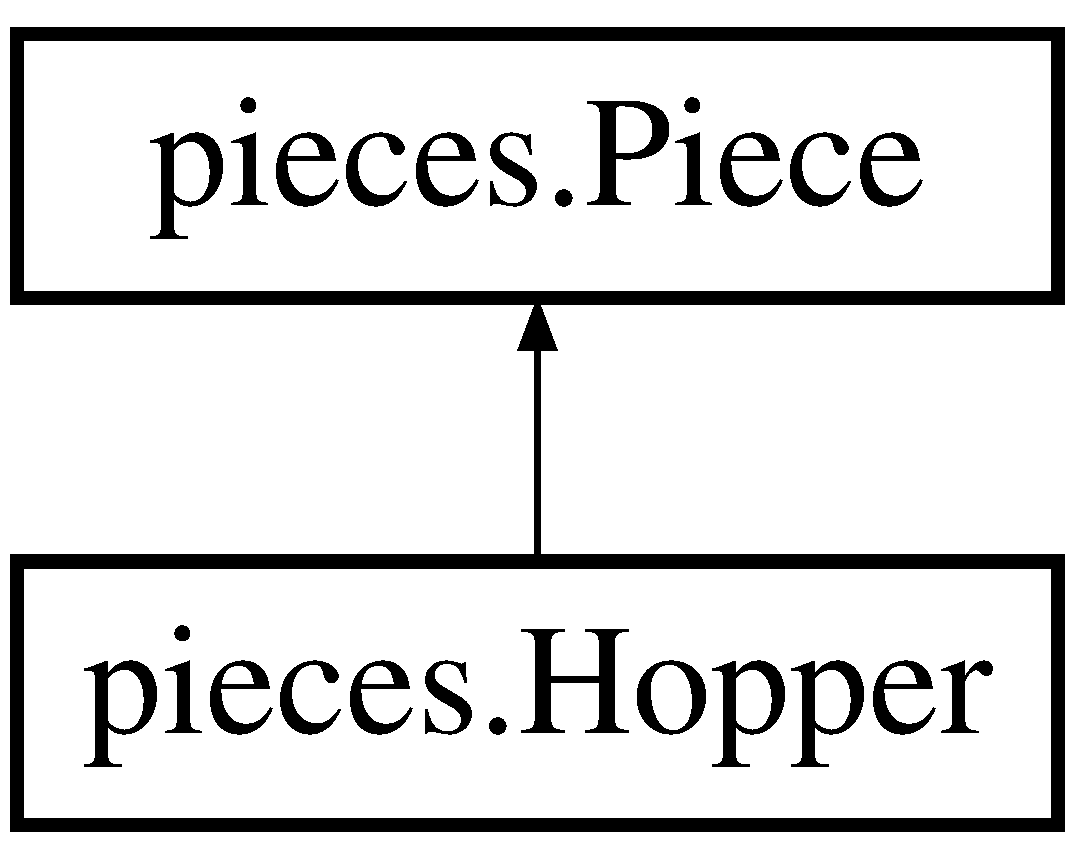
\includegraphics[height=2.000000cm]{classpieces_1_1_hopper}
\end{center}
\end{figure}
\subsection*{Public Member Functions}
\begin{DoxyCompactItemize}
\item 
\mbox{\Hypertarget{classpieces_1_1_hopper_a11e903d52e8635b68167df64addd4d69}\label{classpieces_1_1_hopper_a11e903d52e8635b68167df64addd4d69}} 
{\bfseries Hopper} (\mbox{\hyperlink{enumpieces_1_1_piece_1_1_piece_color}{Piece\+Color}} piece\+Color, int row\+Index, int col\+Index)
\item 
\mbox{\Hypertarget{classpieces_1_1_hopper_ab73282e84292df92c6146d9dde65e738}\label{classpieces_1_1_hopper_ab73282e84292df92c6146d9dde65e738}} 
List$<$ \mbox{\hyperlink{classpieces_1_1_move}{Move}} $>$ {\bfseries compute\+Valid\+Moves} (\mbox{\hyperlink{classgameboard_1_1_game_board}{Game\+Board}} board)
\item 
\mbox{\Hypertarget{classpieces_1_1_hopper_a498def214c5db9ec4db24cefcab4d682}\label{classpieces_1_1_hopper_a498def214c5db9ec4db24cefcab4d682}} 
String {\bfseries get\+String} ()
\end{DoxyCompactItemize}
\subsection*{Additional Inherited Members}


\subsection{Detailed Description}
A hopper is a piece that moves by jumping over another piece (called a hurdle). The hurdle can be any piece of any color. Unless it can jump over a piece, a hopper cannot move. It captures by taking the enemy piece on the destination square, 

The documentation for this class was generated from the following file\+:\begin{DoxyCompactItemize}
\item 
src/pieces/Hopper.\+java\end{DoxyCompactItemize}

\hypertarget{classtest_1_1_hopper_test}{}\section{test.\+Hopper\+Test Class Reference}
\label{classtest_1_1_hopper_test}\index{test.\+Hopper\+Test@{test.\+Hopper\+Test}}
Inheritance diagram for test.\+Hopper\+Test\+:\begin{figure}[H]
\begin{center}
\leavevmode
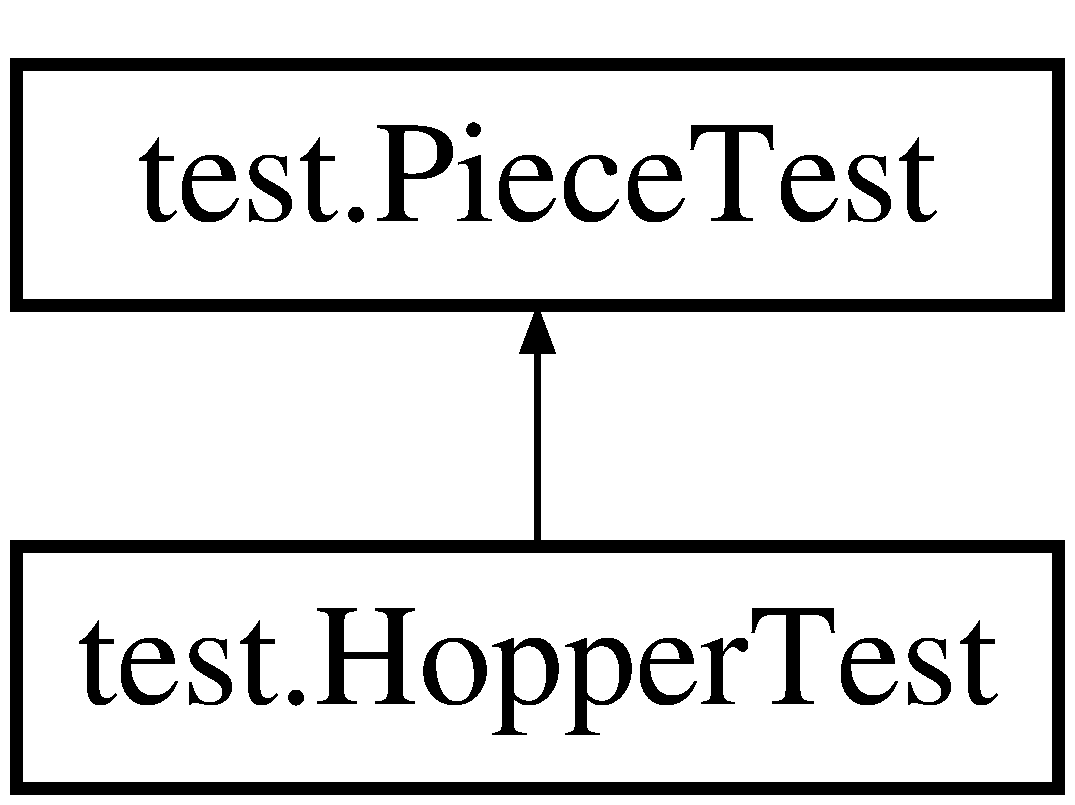
\includegraphics[height=2.000000cm]{classtest_1_1_hopper_test}
\end{center}
\end{figure}
\subsection*{Public Member Functions}
\begin{DoxyCompactItemize}
\item 
\mbox{\Hypertarget{classtest_1_1_hopper_test_aab1273edd7c8652a55cbdfef6ad631fc}\label{classtest_1_1_hopper_test_aab1273edd7c8652a55cbdfef6ad631fc}} 
void {\bfseries Valid\+Constructor2} ()  throws Exception 
\item 
\mbox{\Hypertarget{classtest_1_1_hopper_test_a84532a3a46f32720dc4f69c1f1fc0dc3}\label{classtest_1_1_hopper_test_a84532a3a46f32720dc4f69c1f1fc0dc3}} 
void {\bfseries compute\+Valid\+Moves} ()  throws Exception 
\end{DoxyCompactItemize}
\subsection*{Protected Member Functions}
\begin{DoxyCompactItemize}
\item 
\mbox{\Hypertarget{classtest_1_1_hopper_test_a9d26c802a5dc723cfc67ee6d1b5652e3}\label{classtest_1_1_hopper_test_a9d26c802a5dc723cfc67ee6d1b5652e3}} 
\mbox{\hyperlink{classpieces_1_1_piece}{Piece}} {\bfseries get\+Concrete} (\mbox{\hyperlink{enumpieces_1_1_piece_1_1_piece_color}{Piece.\+Piece\+Color}} piece\+Color, int coordinate\+Row, int coordinate\+Col)
\end{DoxyCompactItemize}
\subsection*{Additional Inherited Members}


\subsection{Detailed Description}
Tests the operations of a Hopper 

The documentation for this class was generated from the following file\+:\begin{DoxyCompactItemize}
\item 
src/test/Hopper\+Test.\+java\end{DoxyCompactItemize}

\hypertarget{classpieces_1_1_king}{}\section{pieces.\+King Class Reference}
\label{classpieces_1_1_king}\index{pieces.\+King@{pieces.\+King}}
Inheritance diagram for pieces.\+King\+:\begin{figure}[H]
\begin{center}
\leavevmode
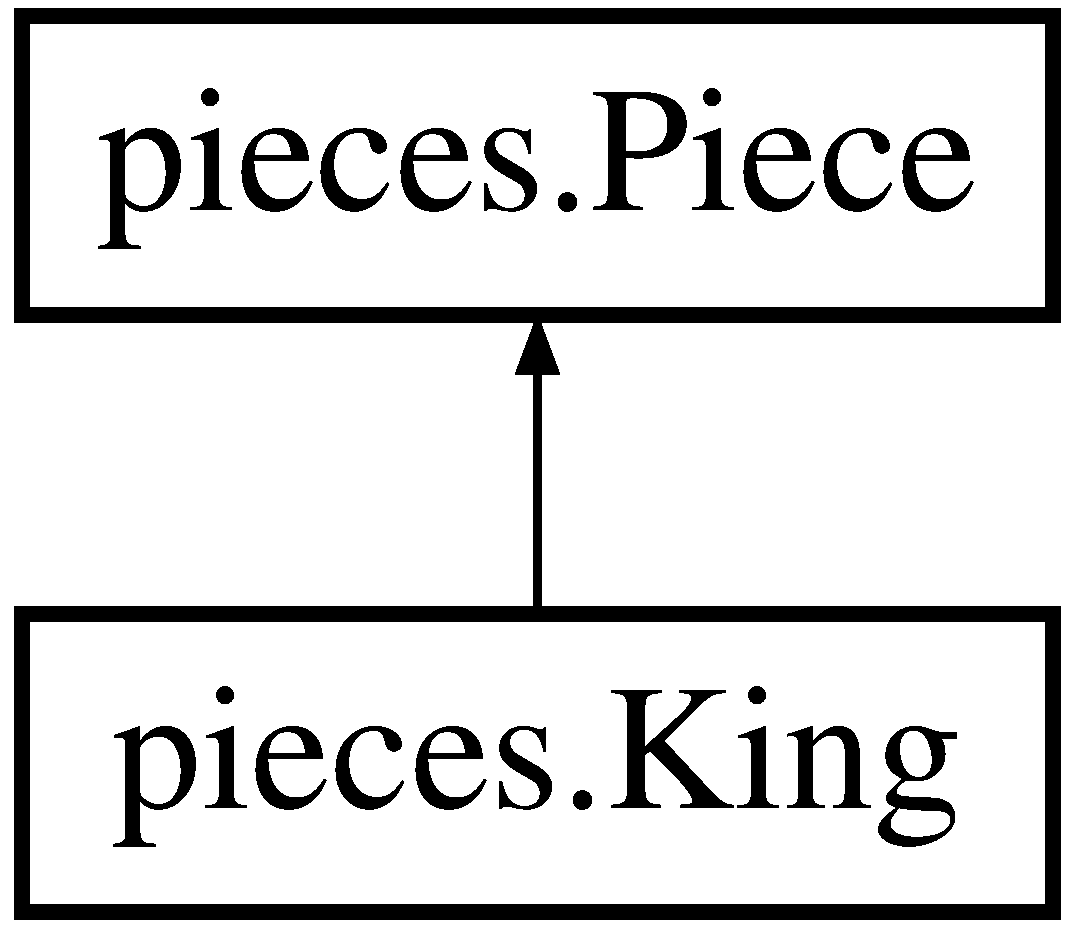
\includegraphics[height=2.000000cm]{classpieces_1_1_king}
\end{center}
\end{figure}
\subsection*{Public Member Functions}
\begin{DoxyCompactItemize}
\item 
\mbox{\Hypertarget{classpieces_1_1_king_a61930731a6bbc9575382f8b64b59b338}\label{classpieces_1_1_king_a61930731a6bbc9575382f8b64b59b338}} 
{\bfseries King} (\mbox{\hyperlink{enumpieces_1_1_piece_1_1_piece_color}{Piece\+Color}} piece\+Color, int coordinate\+Row, int coordinate\+Col)
\item 
\mbox{\Hypertarget{classpieces_1_1_king_a8aa9bef31ee7ffa9f7aabdd8a0f31900}\label{classpieces_1_1_king_a8aa9bef31ee7ffa9f7aabdd8a0f31900}} 
List$<$ \mbox{\hyperlink{classpieces_1_1_move}{Move}} $>$ {\bfseries compute\+Valid\+Moves} (\mbox{\hyperlink{classgameboard_1_1_game_board}{Game\+Board}} board)
\item 
\mbox{\Hypertarget{classpieces_1_1_king_a99f41490f4eeb1380b078c01d100e568}\label{classpieces_1_1_king_a99f41490f4eeb1380b078c01d100e568}} 
String {\bfseries get\+String} ()
\end{DoxyCompactItemize}
\subsection*{Additional Inherited Members}


\subsection{Detailed Description}
Represents a \mbox{\hyperlink{classpieces_1_1_king}{King}} piece of the chess game Created by Siyang\+Liu on 2018/2/2. 

The documentation for this class was generated from the following file\+:\begin{DoxyCompactItemize}
\item 
src/pieces/King.\+java\end{DoxyCompactItemize}

\hypertarget{classtest_1_1_king_test}{}\section{test.\+King\+Test Class Reference}
\label{classtest_1_1_king_test}\index{test.\+King\+Test@{test.\+King\+Test}}
Inheritance diagram for test.\+King\+Test\+:\begin{figure}[H]
\begin{center}
\leavevmode
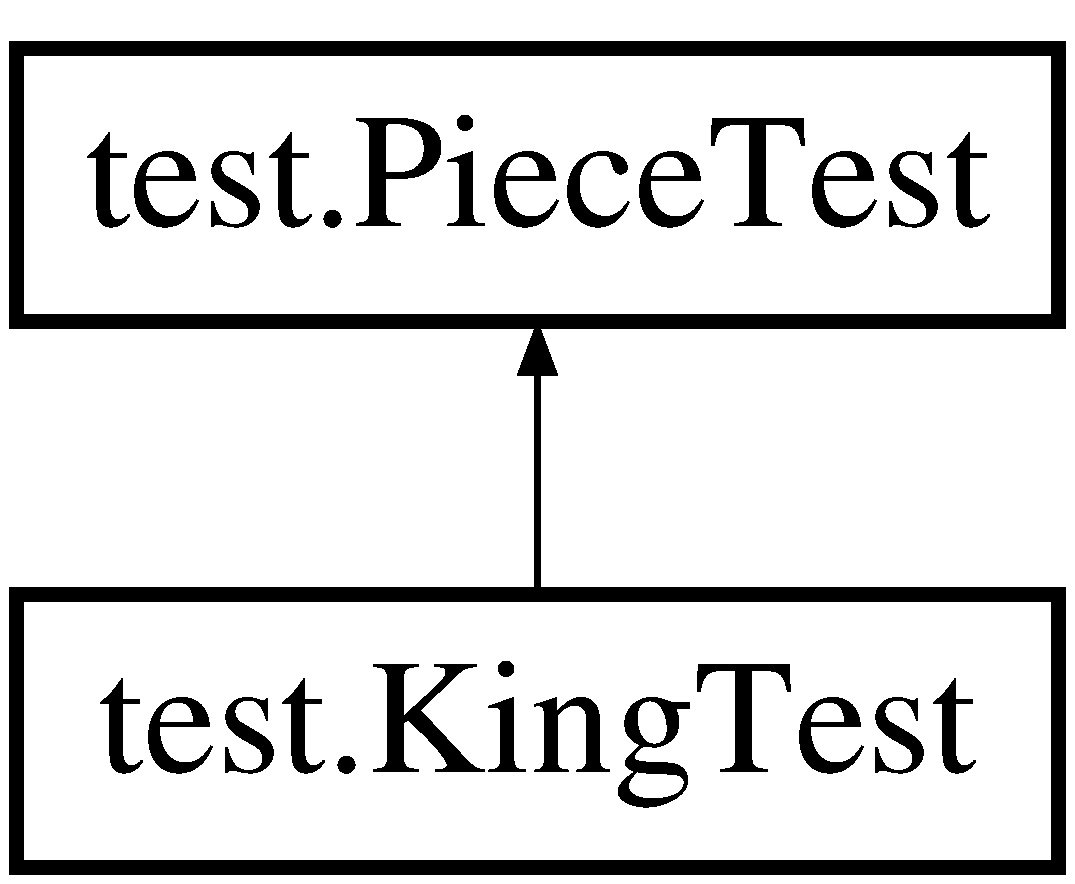
\includegraphics[height=2.000000cm]{classtest_1_1_king_test}
\end{center}
\end{figure}
\subsection*{Public Member Functions}
\begin{DoxyCompactItemize}
\item 
\mbox{\Hypertarget{classtest_1_1_king_test_a8a5a12e9551e74a53bda26babbef2c8f}\label{classtest_1_1_king_test_a8a5a12e9551e74a53bda26babbef2c8f}} 
void {\bfseries compute\+Valid\+Moves} ()  throws Exception 
\item 
\mbox{\Hypertarget{classtest_1_1_king_test_ab2ac93aaf2b3bbfafb242c03791ef729}\label{classtest_1_1_king_test_ab2ac93aaf2b3bbfafb242c03791ef729}} 
void {\bfseries Valid\+Constructor2} ()  throws Exception 
\end{DoxyCompactItemize}
\subsection*{Protected Member Functions}
\begin{DoxyCompactItemize}
\item 
\mbox{\Hypertarget{classtest_1_1_king_test_af74dc8c5229cfb905ad1e81c1003ebc4}\label{classtest_1_1_king_test_af74dc8c5229cfb905ad1e81c1003ebc4}} 
\mbox{\hyperlink{classpieces_1_1_piece}{Piece}} {\bfseries get\+Concrete} (\mbox{\hyperlink{enumpieces_1_1_piece_1_1_piece_color}{Piece.\+Piece\+Color}} piece\+Color, int coordinate\+Row, int coordinate\+Col)
\end{DoxyCompactItemize}
\subsection*{Additional Inherited Members}


\subsection{Detailed Description}
Test for the operations of a King Created by Siyang\+Liu on 2018/2/4. 

The documentation for this class was generated from the following file\+:\begin{DoxyCompactItemize}
\item 
src/test/King\+Test.\+java\end{DoxyCompactItemize}

\hypertarget{classpieces_1_1_knight}{}\section{pieces.\+Knight Class Reference}
\label{classpieces_1_1_knight}\index{pieces.\+Knight@{pieces.\+Knight}}
Inheritance diagram for pieces.\+Knight\+:\begin{figure}[H]
\begin{center}
\leavevmode
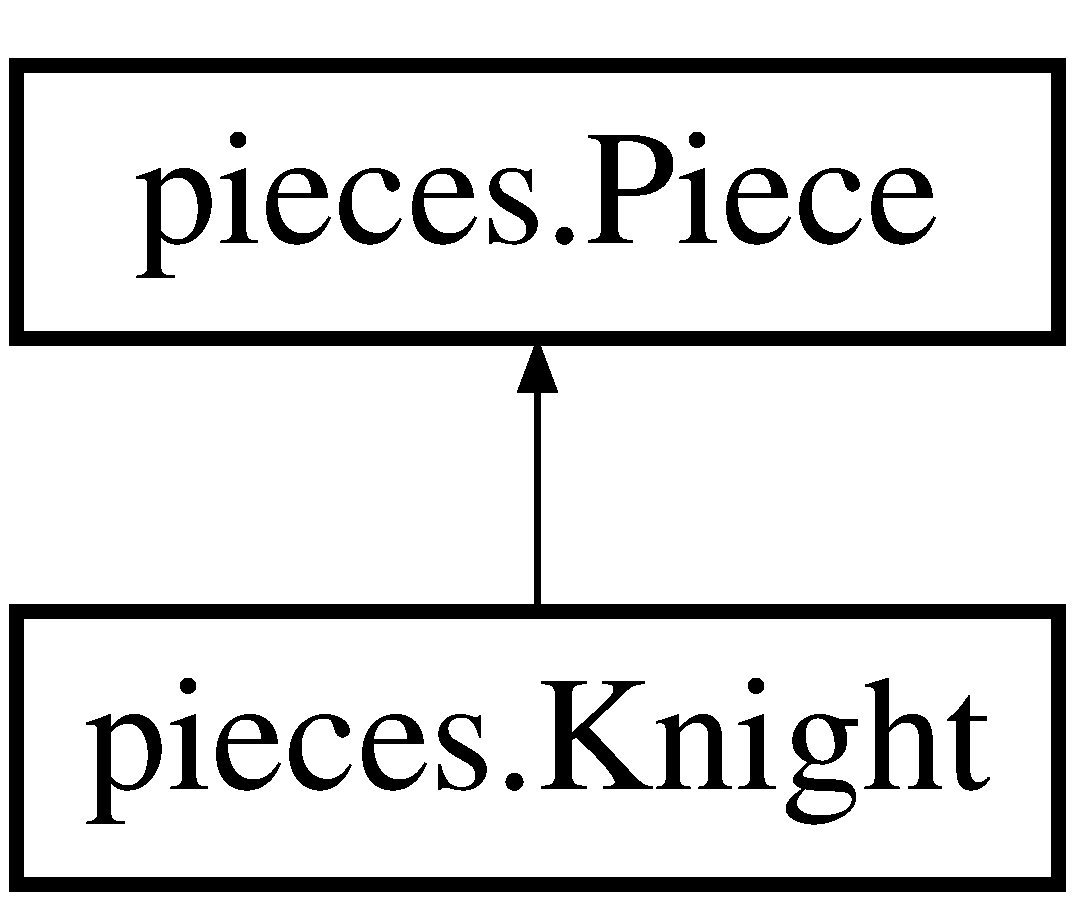
\includegraphics[height=2.000000cm]{classpieces_1_1_knight}
\end{center}
\end{figure}
\subsection*{Public Member Functions}
\begin{DoxyCompactItemize}
\item 
\mbox{\Hypertarget{classpieces_1_1_knight_a35623250e05bc6baac22f422c59bea94}\label{classpieces_1_1_knight_a35623250e05bc6baac22f422c59bea94}} 
{\bfseries Knight} (\mbox{\hyperlink{enumpieces_1_1_piece_1_1_piece_color}{Piece\+Color}} piece\+Color, int coordinate\+Row, int coordinate\+Col)
\item 
\mbox{\Hypertarget{classpieces_1_1_knight_abe3bc9be7e1103cd1ba2ea1cae18a290}\label{classpieces_1_1_knight_abe3bc9be7e1103cd1ba2ea1cae18a290}} 
List$<$ \mbox{\hyperlink{classpieces_1_1_move}{Move}} $>$ {\bfseries compute\+Valid\+Moves} (\mbox{\hyperlink{classgameboard_1_1_game_board}{Game\+Board}} board)
\item 
\mbox{\Hypertarget{classpieces_1_1_knight_a9401a10578ca96dd0cc066195d7bb8fe}\label{classpieces_1_1_knight_a9401a10578ca96dd0cc066195d7bb8fe}} 
String {\bfseries get\+String} ()
\end{DoxyCompactItemize}
\subsection*{Additional Inherited Members}


\subsection{Detailed Description}
Represents a \mbox{\hyperlink{classpieces_1_1_knight}{Knight}} piece of the chess game Created by Siyang\+Liu on 2018/2/2. 

The documentation for this class was generated from the following file\+:\begin{DoxyCompactItemize}
\item 
src/pieces/Knight.\+java\end{DoxyCompactItemize}

\hypertarget{classtest_1_1_knight_test}{}\section{test.\+Knight\+Test Class Reference}
\label{classtest_1_1_knight_test}\index{test.\+Knight\+Test@{test.\+Knight\+Test}}
Inheritance diagram for test.\+Knight\+Test\+:\begin{figure}[H]
\begin{center}
\leavevmode
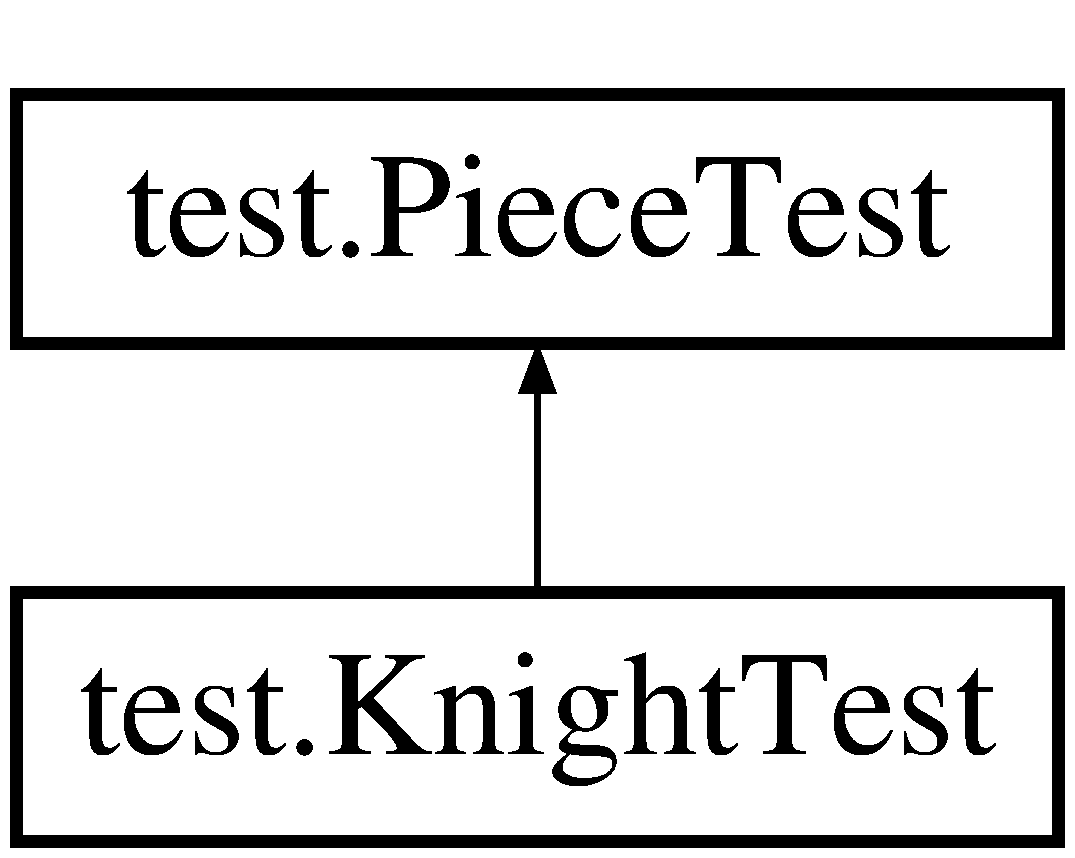
\includegraphics[height=2.000000cm]{classtest_1_1_knight_test}
\end{center}
\end{figure}
\subsection*{Public Member Functions}
\begin{DoxyCompactItemize}
\item 
\mbox{\Hypertarget{classtest_1_1_knight_test_ab1a3e2652086c5437ac7c490edd8d5ae}\label{classtest_1_1_knight_test_ab1a3e2652086c5437ac7c490edd8d5ae}} 
void {\bfseries Valid\+Constructor2} ()  throws Exception 
\item 
\mbox{\Hypertarget{classtest_1_1_knight_test_a1d8d3a0a9ed74cac83cafcf2779e41e8}\label{classtest_1_1_knight_test_a1d8d3a0a9ed74cac83cafcf2779e41e8}} 
void {\bfseries compute\+Valid\+Moves} ()  throws Exception 
\end{DoxyCompactItemize}
\subsection*{Protected Member Functions}
\begin{DoxyCompactItemize}
\item 
\mbox{\Hypertarget{classtest_1_1_knight_test_ab72a9ecbc9dffaacd38c40bedb7a1347}\label{classtest_1_1_knight_test_ab72a9ecbc9dffaacd38c40bedb7a1347}} 
\mbox{\hyperlink{classpieces_1_1_piece}{Piece}} {\bfseries get\+Concrete} (\mbox{\hyperlink{enumpieces_1_1_piece_1_1_piece_color}{Piece.\+Piece\+Color}} piece\+Color, int coordinate\+Row, int coordinate\+Col)
\end{DoxyCompactItemize}
\subsection*{Additional Inherited Members}


\subsection{Detailed Description}
Test for the operations of a Knight Created by Siyang\+Liu on 2018/2/4. 

The documentation for this class was generated from the following file\+:\begin{DoxyCompactItemize}
\item 
src/test/Knight\+Test.\+java\end{DoxyCompactItemize}

\hypertarget{classgui_1_1_main}{}\section{gui.\+Main Class Reference}
\label{classgui_1_1_main}\index{gui.\+Main@{gui.\+Main}}
\subsection*{Static Public Member Functions}
\begin{DoxyCompactItemize}
\item 
static void \mbox{\hyperlink{classgui_1_1_main_a041646fffc0529a864bae17dd55c8514}{main}} (String\mbox{[}$\,$\mbox{]} args)
\end{DoxyCompactItemize}


\subsection{Member Function Documentation}
\mbox{\Hypertarget{classgui_1_1_main_a041646fffc0529a864bae17dd55c8514}\label{classgui_1_1_main_a041646fffc0529a864bae17dd55c8514}} 
\index{gui\+::\+Main@{gui\+::\+Main}!main@{main}}
\index{main@{main}!gui\+::\+Main@{gui\+::\+Main}}
\subsubsection{\texorpdfstring{main()}{main()}}
{\footnotesize\ttfamily static void gui.\+Main.\+main (\begin{DoxyParamCaption}\item[{String \mbox{[}$\,$\mbox{]}}]{args }\end{DoxyParamCaption})\hspace{0.3cm}{\ttfamily [static]}}

the start of the chess program 
\begin{DoxyParams}{Parameters}
{\em args} & \\
\hline
\end{DoxyParams}


The documentation for this class was generated from the following file\+:\begin{DoxyCompactItemize}
\item 
src/gui/Main.\+java\end{DoxyCompactItemize}

\hypertarget{classpieces_1_1_move}{}\section{pieces.\+Move Class Reference}
\label{classpieces_1_1_move}\index{pieces.\+Move@{pieces.\+Move}}
\subsection*{Public Member Functions}
\begin{DoxyCompactItemize}
\item 
\mbox{\Hypertarget{classpieces_1_1_move_a9d8c8259fe150576a61ab1bf8448cb6f}\label{classpieces_1_1_move_a9d8c8259fe150576a61ab1bf8448cb6f}} 
{\bfseries Move} (\mbox{\hyperlink{classpieces_1_1_piece}{Piece}} piece, int dest\+Row, int dest\+Col, \mbox{\hyperlink{classpieces_1_1_piece}{Piece}} to\+Capture)
\item 
\mbox{\Hypertarget{classpieces_1_1_move_ae751299c10522a5e08447b384958b583}\label{classpieces_1_1_move_ae751299c10522a5e08447b384958b583}} 
boolean {\bfseries equals} (Object o)
\item 
\mbox{\Hypertarget{classpieces_1_1_move_a4c1107627a4388558d5d340fa7a49e4a}\label{classpieces_1_1_move_a4c1107627a4388558d5d340fa7a49e4a}} 
\mbox{\hyperlink{classpieces_1_1_piece}{Piece}} {\bfseries get\+Piece} ()
\item 
\mbox{\Hypertarget{classpieces_1_1_move_a7462ffdd4e91afeeacaba11a22d13cea}\label{classpieces_1_1_move_a7462ffdd4e91afeeacaba11a22d13cea}} 
int {\bfseries get\+Dest\+Row} ()
\item 
\mbox{\Hypertarget{classpieces_1_1_move_ad220de4832908acb96959e39812e3d8c}\label{classpieces_1_1_move_ad220de4832908acb96959e39812e3d8c}} 
int {\bfseries get\+Dest\+Col} ()
\item 
\mbox{\Hypertarget{classpieces_1_1_move_a98ad8ca1d7fedb3e09af48a72e76ade1}\label{classpieces_1_1_move_a98ad8ca1d7fedb3e09af48a72e76ade1}} 
int {\bfseries get\+Start\+Row} ()
\item 
\mbox{\Hypertarget{classpieces_1_1_move_ac0f85bd255bb8a5984537b4267665839}\label{classpieces_1_1_move_ac0f85bd255bb8a5984537b4267665839}} 
int {\bfseries get\+Start\+Col} ()
\item 
\mbox{\Hypertarget{classpieces_1_1_move_af78d432f0d3ac098ae38c6a5a1512a12}\label{classpieces_1_1_move_af78d432f0d3ac098ae38c6a5a1512a12}} 
\mbox{\hyperlink{classpieces_1_1_piece}{Piece}} {\bfseries get\+To\+Capture} ()
\end{DoxyCompactItemize}


\subsection{Detailed Description}
guaranteed to be valid update\+Piece\+Coordinates Created by Siyang\+Liu on 2018/2/3. 

The documentation for this class was generated from the following file\+:\begin{DoxyCompactItemize}
\item 
src/pieces/Move.\+java\end{DoxyCompactItemize}

\hypertarget{classtest_1_1_move_test}{}\section{test.\+Move\+Test Class Reference}
\label{classtest_1_1_move_test}\index{test.\+Move\+Test@{test.\+Move\+Test}}
\subsection*{Public Member Functions}
\begin{DoxyCompactItemize}
\item 
void \mbox{\hyperlink{classtest_1_1_move_test_a80a01eeb7d7f45416b2b14f28b44eea0}{test\+Equals}} ()
\end{DoxyCompactItemize}


\subsection{Detailed Description}
Test for the operations of a Move object Created by Siyang\+Liu on 2018/2/4. 

\subsection{Member Function Documentation}
\mbox{\Hypertarget{classtest_1_1_move_test_a80a01eeb7d7f45416b2b14f28b44eea0}\label{classtest_1_1_move_test_a80a01eeb7d7f45416b2b14f28b44eea0}} 
\index{test\+::\+Move\+Test@{test\+::\+Move\+Test}!test\+Equals@{test\+Equals}}
\index{test\+Equals@{test\+Equals}!test\+::\+Move\+Test@{test\+::\+Move\+Test}}
\subsubsection{\texorpdfstring{test\+Equals()}{testEquals()}}
{\footnotesize\ttfamily void test.\+Move\+Test.\+test\+Equals (\begin{DoxyParamCaption}{ }\end{DoxyParamCaption})}

Tests if equals() is correctly overridden for Move object 

The documentation for this class was generated from the following file\+:\begin{DoxyCompactItemize}
\item 
src/test/Move\+Test.\+java\end{DoxyCompactItemize}

\hypertarget{classpieces_1_1_pawn}{}\section{pieces.\+Pawn Class Reference}
\label{classpieces_1_1_pawn}\index{pieces.\+Pawn@{pieces.\+Pawn}}
Inheritance diagram for pieces.\+Pawn\+:\begin{figure}[H]
\begin{center}
\leavevmode
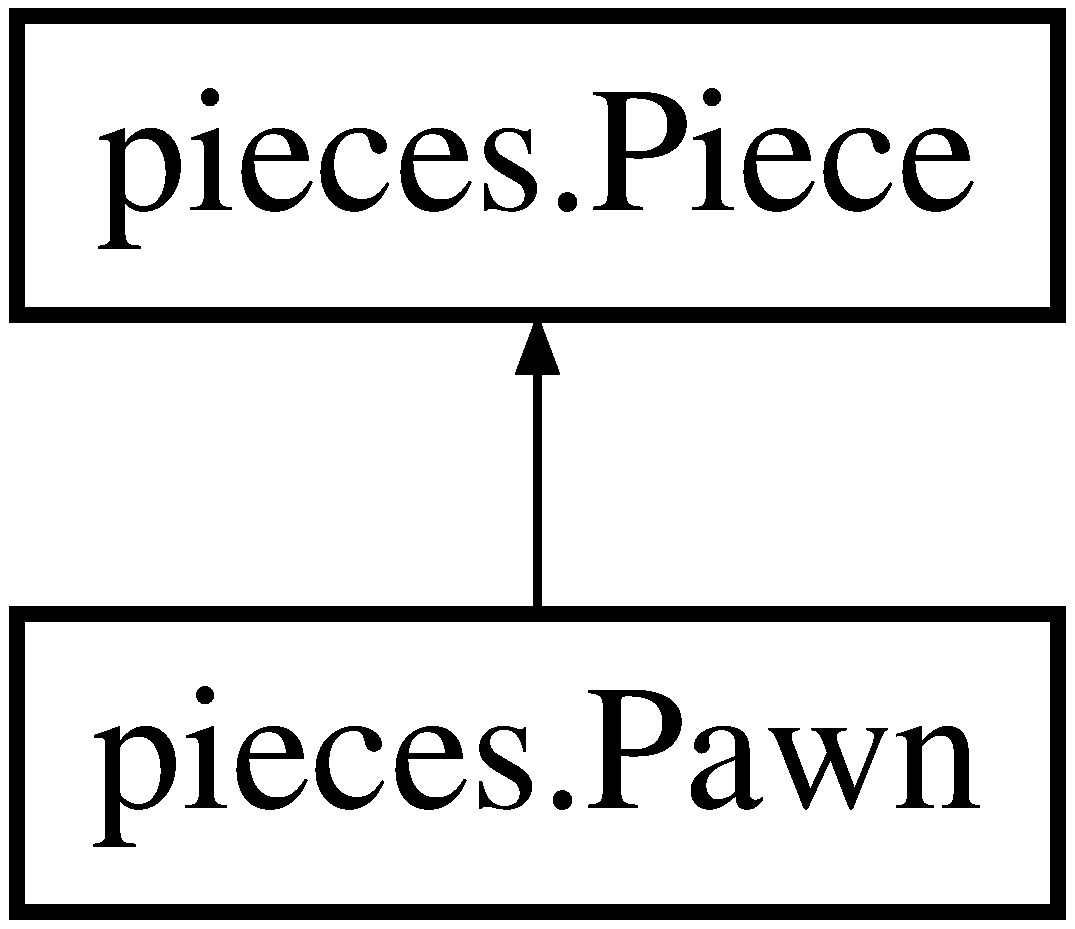
\includegraphics[height=2.000000cm]{classpieces_1_1_pawn}
\end{center}
\end{figure}
\subsection*{Public Member Functions}
\begin{DoxyCompactItemize}
\item 
\mbox{\Hypertarget{classpieces_1_1_pawn_a9165001fee7b0262ff08161b7d03f3c4}\label{classpieces_1_1_pawn_a9165001fee7b0262ff08161b7d03f3c4}} 
{\bfseries Pawn} (\mbox{\hyperlink{enumpieces_1_1_piece_1_1_piece_color}{Piece\+Color}} piece\+Color, int coordinate\+Row, int coordinate\+Col)
\item 
\mbox{\Hypertarget{classpieces_1_1_pawn_abbe6d7f66832496c1ae371d28531d608}\label{classpieces_1_1_pawn_abbe6d7f66832496c1ae371d28531d608}} 
void {\bfseries update\+Piece\+Coordinates} (int dest\+Row, int dest\+Col)
\item 
\mbox{\Hypertarget{classpieces_1_1_pawn_a1e49de35e9aec99eb704e9a9b3311e82}\label{classpieces_1_1_pawn_a1e49de35e9aec99eb704e9a9b3311e82}} 
List$<$ \mbox{\hyperlink{classpieces_1_1_move}{Move}} $>$ {\bfseries compute\+Valid\+Moves} (\mbox{\hyperlink{classgameboard_1_1_game_board}{Game\+Board}} board)
\item 
\mbox{\Hypertarget{classpieces_1_1_pawn_af16853a3b9916d98f9874ccbceacee27}\label{classpieces_1_1_pawn_af16853a3b9916d98f9874ccbceacee27}} 
boolean {\bfseries is\+First\+Move} ()
\item 
\mbox{\Hypertarget{classpieces_1_1_pawn_ae5bfb4aa4e9fbbe23c313a34ba628175}\label{classpieces_1_1_pawn_ae5bfb4aa4e9fbbe23c313a34ba628175}} 
String {\bfseries get\+String} ()
\end{DoxyCompactItemize}
\subsection*{Additional Inherited Members}


\subsection{Detailed Description}
Represents a \mbox{\hyperlink{classpieces_1_1_pawn}{Pawn}} piece of the chess game Created by Siyang\+Liu on 2018/2/2. 

The documentation for this class was generated from the following file\+:\begin{DoxyCompactItemize}
\item 
src/pieces/Pawn.\+java\end{DoxyCompactItemize}

\hypertarget{classtest_1_1_pawn_test}{}\section{test.\+Pawn\+Test Class Reference}
\label{classtest_1_1_pawn_test}\index{test.\+Pawn\+Test@{test.\+Pawn\+Test}}
Inheritance diagram for test.\+Pawn\+Test\+:\begin{figure}[H]
\begin{center}
\leavevmode
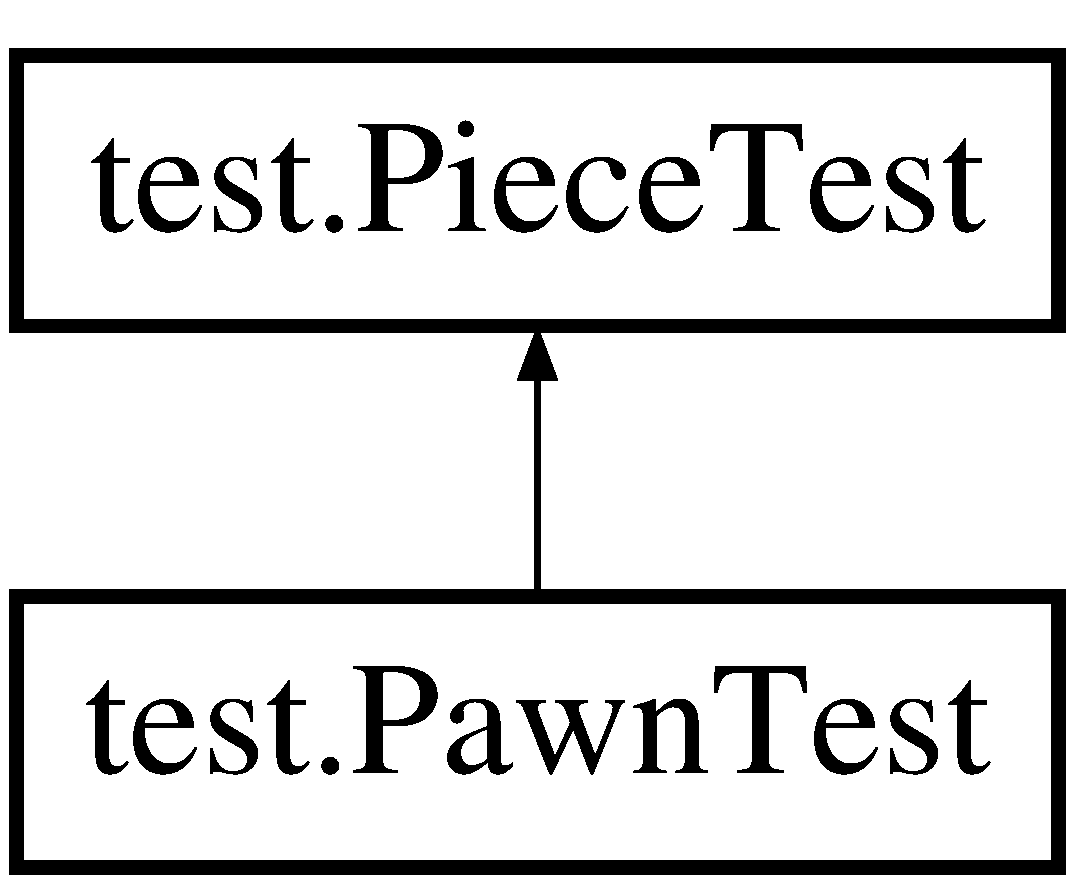
\includegraphics[height=2.000000cm]{classtest_1_1_pawn_test}
\end{center}
\end{figure}
\subsection*{Public Member Functions}
\begin{DoxyCompactItemize}
\item 
\mbox{\Hypertarget{classtest_1_1_pawn_test_ac43e71ec6827ee2dede95103f600752b}\label{classtest_1_1_pawn_test_ac43e71ec6827ee2dede95103f600752b}} 
void {\bfseries Valid\+Constructor2} ()  throws Exception 
\item 
\mbox{\Hypertarget{classtest_1_1_pawn_test_a6c5484d6c801d4ce7ba09d6a45aad74f}\label{classtest_1_1_pawn_test_a6c5484d6c801d4ce7ba09d6a45aad74f}} 
void {\bfseries compute\+Valid\+Moves} ()  throws Exception 
\end{DoxyCompactItemize}
\subsection*{Protected Member Functions}
\begin{DoxyCompactItemize}
\item 
\mbox{\Hypertarget{classtest_1_1_pawn_test_aa53df44fa4d9b2e462a0be226bfb7ccc}\label{classtest_1_1_pawn_test_aa53df44fa4d9b2e462a0be226bfb7ccc}} 
\mbox{\hyperlink{classpieces_1_1_piece}{Piece}} {\bfseries get\+Concrete} (Piece.\+Piece\+Color piece\+Color, int coordinate\+Row, int coordinate\+Col)
\end{DoxyCompactItemize}
\subsection*{Additional Inherited Members}


\subsection{Detailed Description}
Test for the operations of a Pawn Created by Siyang\+Liu on 2018/2/4. 

The documentation for this class was generated from the following file\+:\begin{DoxyCompactItemize}
\item 
src/test/Pawn\+Test.\+java\end{DoxyCompactItemize}

\hypertarget{classpieces_1_1_piece}{}\section{pieces.\+Piece Class Reference}
\label{classpieces_1_1_piece}\index{pieces.\+Piece@{pieces.\+Piece}}
Inheritance diagram for pieces.\+Piece\+:\begin{figure}[H]
\begin{center}
\leavevmode
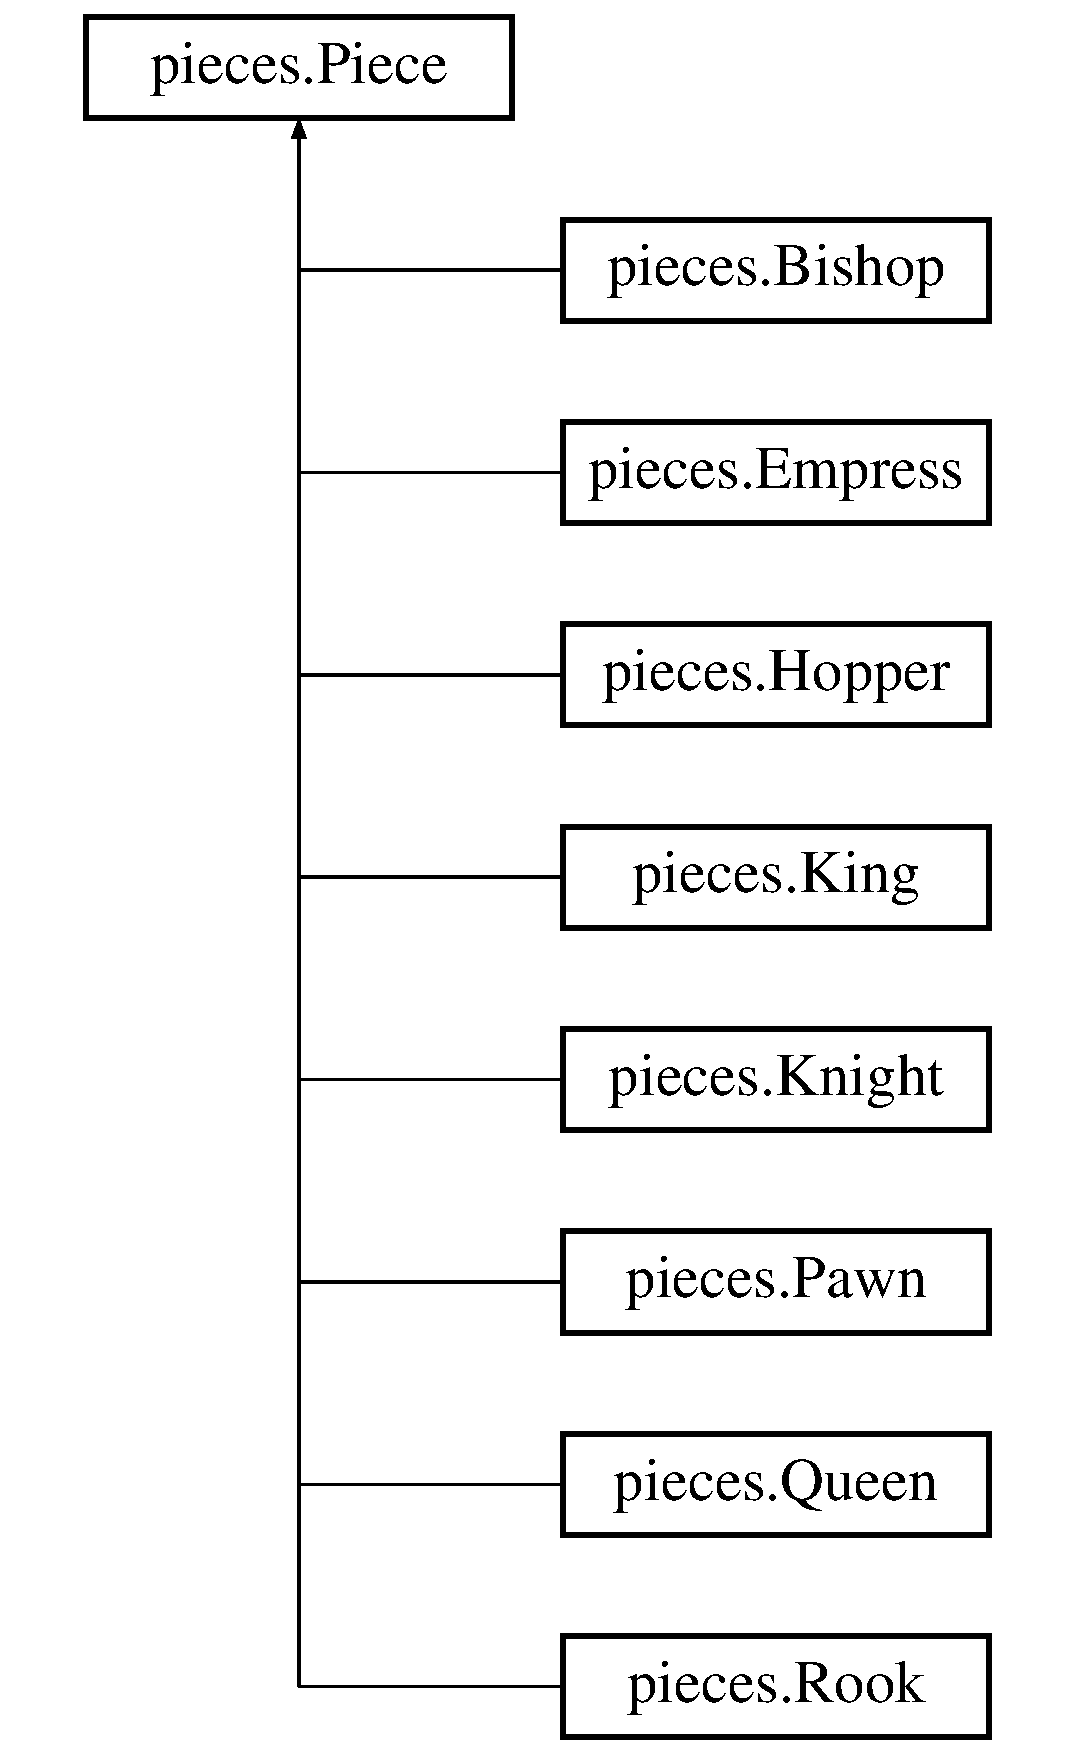
\includegraphics[height=9.000000cm]{classpieces_1_1_piece}
\end{center}
\end{figure}
\subsection*{Classes}
\begin{DoxyCompactItemize}
\item 
enum \mbox{\hyperlink{enumpieces_1_1_piece_1_1_piece_color}{Piece\+Color}}
\item 
enum \mbox{\hyperlink{enumpieces_1_1_piece_1_1_piece_type}{Piece\+Type}}
\end{DoxyCompactItemize}
\subsection*{Public Member Functions}
\begin{DoxyCompactItemize}
\item 
boolean \mbox{\hyperlink{classpieces_1_1_piece_a24536ff95674905f18a7fd9fadde52ce}{is\+Valid\+Move}} (\mbox{\hyperlink{classpieces_1_1_move}{Move}} move)
\item 
abstract List$<$ \mbox{\hyperlink{classpieces_1_1_move}{Move}} $>$ \mbox{\hyperlink{classpieces_1_1_piece_ab9a0e46deaaa05e8bea7a59ccda801ab}{compute\+Valid\+Moves}} (final \mbox{\hyperlink{classgameboard_1_1_game_board}{Game\+Board}} board)
\item 
void \mbox{\hyperlink{classpieces_1_1_piece_abad4a76991f2de3a31187c2a74c2f870}{update\+Piece\+Coordinates}} (int dest\+Row, int dest\+Col)
\item 
\mbox{\hyperlink{enumpieces_1_1_piece_1_1_piece_color}{Piece\+Color}} \mbox{\hyperlink{classpieces_1_1_piece_a3442ea119c005e9736d5cd53efd499e8}{get\+Piece\+Color}} ()
\item 
\mbox{\hyperlink{enumpieces_1_1_piece_1_1_piece_type}{Piece\+Type}} \mbox{\hyperlink{classpieces_1_1_piece_acd116a1f6e774bc7d358780c098fadcb}{get\+Piece\+Type}} ()
\item 
abstract String \mbox{\hyperlink{classpieces_1_1_piece_a12cbd905036c427015bd3c62fdb17036}{get\+String}} ()
\item 
int \mbox{\hyperlink{classpieces_1_1_piece_a298b5268de024c41b2af48306fa40e03}{get\+Row\+Index}} ()
\item 
int \mbox{\hyperlink{classpieces_1_1_piece_a5ac1137f5b634718b310ba4b01d3a592}{get\+Col\+Index}} ()
\item 
List$<$ \mbox{\hyperlink{classpieces_1_1_move}{Move}} $>$ \mbox{\hyperlink{classpieces_1_1_piece_aa4bfcbf5e6e3c1374c0ca3af0c64b87d}{get\+Valid\+Moves}} ()
\end{DoxyCompactItemize}
\subsection*{Protected Member Functions}
\begin{DoxyCompactItemize}
\item 
\mbox{\Hypertarget{classpieces_1_1_piece_aa02280c819d5ab7472b50a1026ca2e9d}\label{classpieces_1_1_piece_aa02280c819d5ab7472b50a1026ca2e9d}} 
{\bfseries Piece} (\mbox{\hyperlink{enumpieces_1_1_piece_1_1_piece_color}{Piece\+Color}} piece\+Color, int row\+Index, int col\+Index)
\end{DoxyCompactItemize}


\subsection{Detailed Description}
Represents a piece in the chess game Created by Siyang\+Liu on 2018/2/2. 

\subsection{Member Function Documentation}
\mbox{\Hypertarget{classpieces_1_1_piece_ab9a0e46deaaa05e8bea7a59ccda801ab}\label{classpieces_1_1_piece_ab9a0e46deaaa05e8bea7a59ccda801ab}} 
\index{pieces\+::\+Piece@{pieces\+::\+Piece}!compute\+Valid\+Moves@{compute\+Valid\+Moves}}
\index{compute\+Valid\+Moves@{compute\+Valid\+Moves}!pieces\+::\+Piece@{pieces\+::\+Piece}}
\subsubsection{\texorpdfstring{compute\+Valid\+Moves()}{computeValidMoves()}}
{\footnotesize\ttfamily abstract List$<$\mbox{\hyperlink{classpieces_1_1_move}{Move}}$>$ pieces.\+Piece.\+compute\+Valid\+Moves (\begin{DoxyParamCaption}\item[{final \mbox{\hyperlink{classgameboard_1_1_game_board}{Game\+Board}}}]{board }\end{DoxyParamCaption})\hspace{0.3cm}{\ttfamily [abstract]}}

Computes all valid moves of the piece given the current board \mbox{\Hypertarget{classpieces_1_1_piece_a5ac1137f5b634718b310ba4b01d3a592}\label{classpieces_1_1_piece_a5ac1137f5b634718b310ba4b01d3a592}} 
\index{pieces\+::\+Piece@{pieces\+::\+Piece}!get\+Col\+Index@{get\+Col\+Index}}
\index{get\+Col\+Index@{get\+Col\+Index}!pieces\+::\+Piece@{pieces\+::\+Piece}}
\subsubsection{\texorpdfstring{get\+Col\+Index()}{getColIndex()}}
{\footnotesize\ttfamily int pieces.\+Piece.\+get\+Col\+Index (\begin{DoxyParamCaption}{ }\end{DoxyParamCaption})}

Gets the column index of the piece in the board \mbox{\Hypertarget{classpieces_1_1_piece_a3442ea119c005e9736d5cd53efd499e8}\label{classpieces_1_1_piece_a3442ea119c005e9736d5cd53efd499e8}} 
\index{pieces\+::\+Piece@{pieces\+::\+Piece}!get\+Piece\+Color@{get\+Piece\+Color}}
\index{get\+Piece\+Color@{get\+Piece\+Color}!pieces\+::\+Piece@{pieces\+::\+Piece}}
\subsubsection{\texorpdfstring{get\+Piece\+Color()}{getPieceColor()}}
{\footnotesize\ttfamily \mbox{\hyperlink{enumpieces_1_1_piece_1_1_piece_color}{Piece\+Color}} pieces.\+Piece.\+get\+Piece\+Color (\begin{DoxyParamCaption}{ }\end{DoxyParamCaption})}

Gets the color of the piece \mbox{\Hypertarget{classpieces_1_1_piece_acd116a1f6e774bc7d358780c098fadcb}\label{classpieces_1_1_piece_acd116a1f6e774bc7d358780c098fadcb}} 
\index{pieces\+::\+Piece@{pieces\+::\+Piece}!get\+Piece\+Type@{get\+Piece\+Type}}
\index{get\+Piece\+Type@{get\+Piece\+Type}!pieces\+::\+Piece@{pieces\+::\+Piece}}
\subsubsection{\texorpdfstring{get\+Piece\+Type()}{getPieceType()}}
{\footnotesize\ttfamily \mbox{\hyperlink{enumpieces_1_1_piece_1_1_piece_type}{Piece\+Type}} pieces.\+Piece.\+get\+Piece\+Type (\begin{DoxyParamCaption}{ }\end{DoxyParamCaption})}

Gets the type of the piece \mbox{\Hypertarget{classpieces_1_1_piece_a298b5268de024c41b2af48306fa40e03}\label{classpieces_1_1_piece_a298b5268de024c41b2af48306fa40e03}} 
\index{pieces\+::\+Piece@{pieces\+::\+Piece}!get\+Row\+Index@{get\+Row\+Index}}
\index{get\+Row\+Index@{get\+Row\+Index}!pieces\+::\+Piece@{pieces\+::\+Piece}}
\subsubsection{\texorpdfstring{get\+Row\+Index()}{getRowIndex()}}
{\footnotesize\ttfamily int pieces.\+Piece.\+get\+Row\+Index (\begin{DoxyParamCaption}{ }\end{DoxyParamCaption})}

Gets the row index of the piece in the board \mbox{\Hypertarget{classpieces_1_1_piece_a12cbd905036c427015bd3c62fdb17036}\label{classpieces_1_1_piece_a12cbd905036c427015bd3c62fdb17036}} 
\index{pieces\+::\+Piece@{pieces\+::\+Piece}!get\+String@{get\+String}}
\index{get\+String@{get\+String}!pieces\+::\+Piece@{pieces\+::\+Piece}}
\subsubsection{\texorpdfstring{get\+String()}{getString()}}
{\footnotesize\ttfamily abstract String pieces.\+Piece.\+get\+String (\begin{DoxyParamCaption}{ }\end{DoxyParamCaption})\hspace{0.3cm}{\ttfamily [abstract]}}

Gets the string of the piece all lower case with \+\_\+ between color and type \mbox{\Hypertarget{classpieces_1_1_piece_aa4bfcbf5e6e3c1374c0ca3af0c64b87d}\label{classpieces_1_1_piece_aa4bfcbf5e6e3c1374c0ca3af0c64b87d}} 
\index{pieces\+::\+Piece@{pieces\+::\+Piece}!get\+Valid\+Moves@{get\+Valid\+Moves}}
\index{get\+Valid\+Moves@{get\+Valid\+Moves}!pieces\+::\+Piece@{pieces\+::\+Piece}}
\subsubsection{\texorpdfstring{get\+Valid\+Moves()}{getValidMoves()}}
{\footnotesize\ttfamily List$<$\mbox{\hyperlink{classpieces_1_1_move}{Move}}$>$ pieces.\+Piece.\+get\+Valid\+Moves (\begin{DoxyParamCaption}{ }\end{DoxyParamCaption})}

Gets the valid moves of the piece in the board \mbox{\Hypertarget{classpieces_1_1_piece_a24536ff95674905f18a7fd9fadde52ce}\label{classpieces_1_1_piece_a24536ff95674905f18a7fd9fadde52ce}} 
\index{pieces\+::\+Piece@{pieces\+::\+Piece}!is\+Valid\+Move@{is\+Valid\+Move}}
\index{is\+Valid\+Move@{is\+Valid\+Move}!pieces\+::\+Piece@{pieces\+::\+Piece}}
\subsubsection{\texorpdfstring{is\+Valid\+Move()}{isValidMove()}}
{\footnotesize\ttfamily boolean pieces.\+Piece.\+is\+Valid\+Move (\begin{DoxyParamCaption}\item[{\mbox{\hyperlink{classpieces_1_1_move}{Move}}}]{move }\end{DoxyParamCaption})}

Checks if the move of the piece is valid \mbox{\Hypertarget{classpieces_1_1_piece_abad4a76991f2de3a31187c2a74c2f870}\label{classpieces_1_1_piece_abad4a76991f2de3a31187c2a74c2f870}} 
\index{pieces\+::\+Piece@{pieces\+::\+Piece}!update\+Piece\+Coordinates@{update\+Piece\+Coordinates}}
\index{update\+Piece\+Coordinates@{update\+Piece\+Coordinates}!pieces\+::\+Piece@{pieces\+::\+Piece}}
\subsubsection{\texorpdfstring{update\+Piece\+Coordinates()}{updatePieceCoordinates()}}
{\footnotesize\ttfamily void pieces.\+Piece.\+update\+Piece\+Coordinates (\begin{DoxyParamCaption}\item[{int}]{dest\+Row,  }\item[{int}]{dest\+Col }\end{DoxyParamCaption})}

Updates the coordinates of the piece in the game board Has to follow up with the call to compute\+Valid\+Moves(board) to update the piece 
\begin{DoxyParams}{Parameters}
{\em dest\+Row} & guaranteed to be valid row \\
\hline
{\em dest\+Col} & guaranteed to be valid col \\
\hline
\end{DoxyParams}


The documentation for this class was generated from the following file\+:\begin{DoxyCompactItemize}
\item 
src/pieces/Piece.\+java\end{DoxyCompactItemize}

\hypertarget{enumpieces_1_1_piece_1_1_piece_color}{}\section{pieces.\+Piece.\+Piece\+Color Enum Reference}
\label{enumpieces_1_1_piece_1_1_piece_color}\index{pieces.\+Piece.\+Piece\+Color@{pieces.\+Piece.\+Piece\+Color}}
\subsection*{Public Attributes}
\begin{DoxyCompactItemize}
\item 
\mbox{\Hypertarget{enumpieces_1_1_piece_1_1_piece_color_a936833f5f6ffb9d58752b1dbc9efcbde}\label{enumpieces_1_1_piece_1_1_piece_color_a936833f5f6ffb9d58752b1dbc9efcbde}} 
{\bfseries W\+H\+I\+TE}
\item 
\mbox{\Hypertarget{enumpieces_1_1_piece_1_1_piece_color_ab720fe34a5ee1d4f2d64c8d32a276a09}\label{enumpieces_1_1_piece_1_1_piece_color_ab720fe34a5ee1d4f2d64c8d32a276a09}} 
{\bfseries B\+L\+A\+CK}
\end{DoxyCompactItemize}


\subsection{Detailed Description}
Enumerates all possible colors of a piece 

The documentation for this enum was generated from the following file\+:\begin{DoxyCompactItemize}
\item 
src/pieces/Piece.\+java\end{DoxyCompactItemize}

\hypertarget{classtest_1_1_piece_test}{}\section{test.\+Piece\+Test Class Reference}
\label{classtest_1_1_piece_test}\index{test.\+Piece\+Test@{test.\+Piece\+Test}}
Inheritance diagram for test.\+Piece\+Test\+:\begin{figure}[H]
\begin{center}
\leavevmode
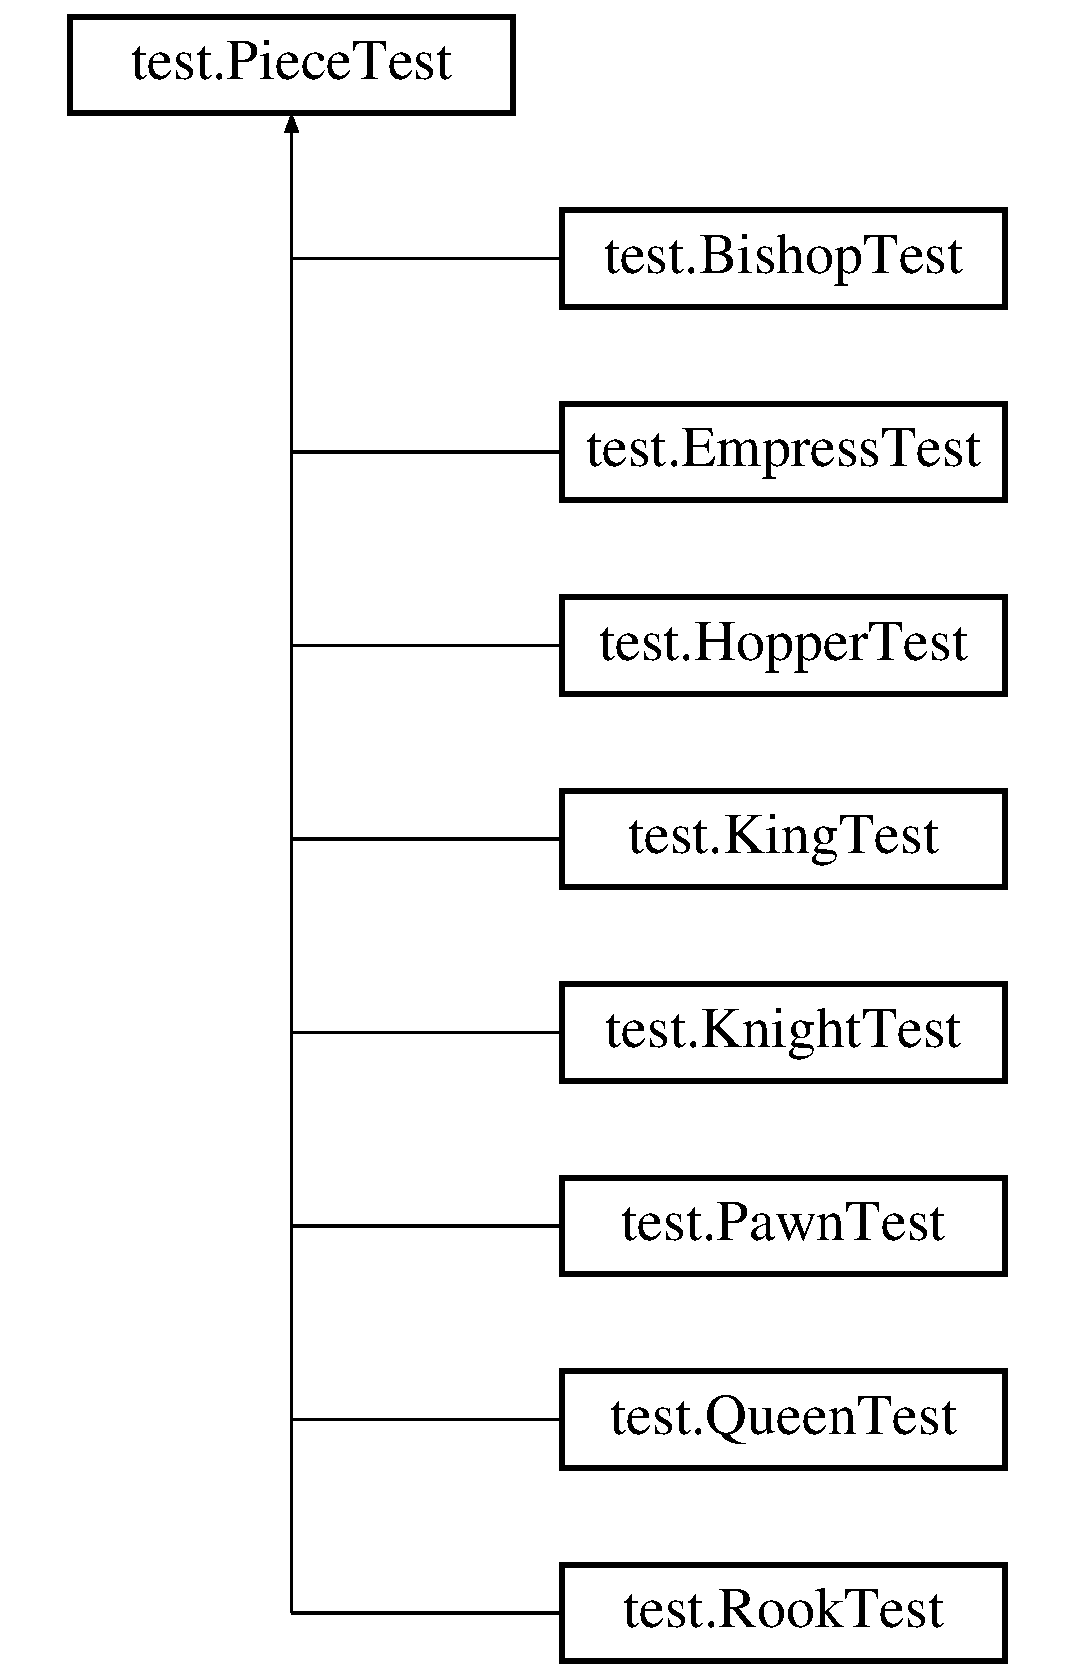
\includegraphics[height=9.000000cm]{classtest_1_1_piece_test}
\end{center}
\end{figure}
\subsection*{Public Member Functions}
\begin{DoxyCompactItemize}
\item 
\mbox{\Hypertarget{classtest_1_1_piece_test_a334090be857c7b0085466dd784768748}\label{classtest_1_1_piece_test_a334090be857c7b0085466dd784768748}} 
void {\bfseries build\+Piece\+For\+Testing} ()
\item 
void \mbox{\hyperlink{classtest_1_1_piece_test_a4680ac39911c714af4402657d7b5a3e2}{Valid\+Constructor1}} ()  throws Exception 
\item 
abstract void \mbox{\hyperlink{classtest_1_1_piece_test_a3c841ee578a23ea6162afd09e09434cd}{Valid\+Constructor2}} ()  throws Exception
\item 
void \mbox{\hyperlink{classtest_1_1_piece_test_aaf5df7af55f8bbcb89bd2554b1876709}{move}} ()  throws Exception 
\item 
abstract void \mbox{\hyperlink{classtest_1_1_piece_test_a8d83b20ef3c6fe8d2acd692b8dedb551}{compute\+Valid\+Moves}} ()  throws Exception
\end{DoxyCompactItemize}
\subsection*{Protected Member Functions}
\begin{DoxyCompactItemize}
\item 
abstract \mbox{\hyperlink{classpieces_1_1_piece}{Piece}} \mbox{\hyperlink{classtest_1_1_piece_test_a90a462bad11a172acd27d1b18e21ee15}{get\+Concrete}} (Piece.\+Piece\+Color piece\+Color, int coordinate\+Row, int coordinate\+Col)
\end{DoxyCompactItemize}
\subsection*{Protected Attributes}
\begin{DoxyCompactItemize}
\item 
\mbox{\Hypertarget{classtest_1_1_piece_test_a567392fa471de32c6eee66f3fd6f069b}\label{classtest_1_1_piece_test_a567392fa471de32c6eee66f3fd6f069b}} 
\mbox{\hyperlink{classpieces_1_1_piece}{Piece}} {\bfseries black\+Piece}
\item 
\mbox{\Hypertarget{classtest_1_1_piece_test_a8104ae553d8aa8bc7ec571612b1ee328}\label{classtest_1_1_piece_test_a8104ae553d8aa8bc7ec571612b1ee328}} 
\mbox{\hyperlink{classpieces_1_1_piece}{Piece}} {\bfseries white\+Piece}
\item 
\mbox{\Hypertarget{classtest_1_1_piece_test_a16d1f0aea9e40fc91717bc8c74aaaa2e}\label{classtest_1_1_piece_test_a16d1f0aea9e40fc91717bc8c74aaaa2e}} 
\mbox{\hyperlink{classgameboard_1_1_game_board}{Game\+Board}} {\bfseries board}
\end{DoxyCompactItemize}


\subsection{Detailed Description}
Test for the operations of a Piece Created by Siyang\+Liu on 2018/2/3. 

\subsection{Member Function Documentation}
\mbox{\Hypertarget{classtest_1_1_piece_test_a8d83b20ef3c6fe8d2acd692b8dedb551}\label{classtest_1_1_piece_test_a8d83b20ef3c6fe8d2acd692b8dedb551}} 
\index{test\+::\+Piece\+Test@{test\+::\+Piece\+Test}!compute\+Valid\+Moves@{compute\+Valid\+Moves}}
\index{compute\+Valid\+Moves@{compute\+Valid\+Moves}!test\+::\+Piece\+Test@{test\+::\+Piece\+Test}}
\subsubsection{\texorpdfstring{compute\+Valid\+Moves()}{computeValidMoves()}}
{\footnotesize\ttfamily abstract void test.\+Piece\+Test.\+compute\+Valid\+Moves (\begin{DoxyParamCaption}{ }\end{DoxyParamCaption}) throws Exception\hspace{0.3cm}{\ttfamily [abstract]}}

Test if the all valid moves are computed correctly \mbox{\Hypertarget{classtest_1_1_piece_test_a90a462bad11a172acd27d1b18e21ee15}\label{classtest_1_1_piece_test_a90a462bad11a172acd27d1b18e21ee15}} 
\index{test\+::\+Piece\+Test@{test\+::\+Piece\+Test}!get\+Concrete@{get\+Concrete}}
\index{get\+Concrete@{get\+Concrete}!test\+::\+Piece\+Test@{test\+::\+Piece\+Test}}
\subsubsection{\texorpdfstring{get\+Concrete()}{getConcrete()}}
{\footnotesize\ttfamily abstract \mbox{\hyperlink{classpieces_1_1_piece}{Piece}} test.\+Piece\+Test.\+get\+Concrete (\begin{DoxyParamCaption}\item[{Piece.\+Piece\+Color}]{piece\+Color,  }\item[{int}]{coordinate\+Row,  }\item[{int}]{coordinate\+Col }\end{DoxyParamCaption})\hspace{0.3cm}{\ttfamily [abstract]}, {\ttfamily [protected]}}

Constructs a concrete piece with one of the piece type in chess \mbox{\Hypertarget{classtest_1_1_piece_test_aaf5df7af55f8bbcb89bd2554b1876709}\label{classtest_1_1_piece_test_aaf5df7af55f8bbcb89bd2554b1876709}} 
\index{test\+::\+Piece\+Test@{test\+::\+Piece\+Test}!move@{move}}
\index{move@{move}!test\+::\+Piece\+Test@{test\+::\+Piece\+Test}}
\subsubsection{\texorpdfstring{move()}{move()}}
{\footnotesize\ttfamily void test.\+Piece\+Test.\+move (\begin{DoxyParamCaption}{ }\end{DoxyParamCaption}) throws Exception}

Test if the resulting board is correct after the execute of a valid move \mbox{\Hypertarget{classtest_1_1_piece_test_a4680ac39911c714af4402657d7b5a3e2}\label{classtest_1_1_piece_test_a4680ac39911c714af4402657d7b5a3e2}} 
\index{test\+::\+Piece\+Test@{test\+::\+Piece\+Test}!Valid\+Constructor1@{Valid\+Constructor1}}
\index{Valid\+Constructor1@{Valid\+Constructor1}!test\+::\+Piece\+Test@{test\+::\+Piece\+Test}}
\subsubsection{\texorpdfstring{Valid\+Constructor1()}{ValidConstructor1()}}
{\footnotesize\ttfamily void test.\+Piece\+Test.\+Valid\+Constructor1 (\begin{DoxyParamCaption}{ }\end{DoxyParamCaption}) throws Exception}

test the instance fields except piece\+Type after construction \mbox{\Hypertarget{classtest_1_1_piece_test_a3c841ee578a23ea6162afd09e09434cd}\label{classtest_1_1_piece_test_a3c841ee578a23ea6162afd09e09434cd}} 
\index{test\+::\+Piece\+Test@{test\+::\+Piece\+Test}!Valid\+Constructor2@{Valid\+Constructor2}}
\index{Valid\+Constructor2@{Valid\+Constructor2}!test\+::\+Piece\+Test@{test\+::\+Piece\+Test}}
\subsubsection{\texorpdfstring{Valid\+Constructor2()}{ValidConstructor2()}}
{\footnotesize\ttfamily abstract void test.\+Piece\+Test.\+Valid\+Constructor2 (\begin{DoxyParamCaption}{ }\end{DoxyParamCaption}) throws Exception\hspace{0.3cm}{\ttfamily [abstract]}}

test the piece\+Type field after construction 

The documentation for this class was generated from the following file\+:\begin{DoxyCompactItemize}
\item 
src/test/Piece\+Test.\+java\end{DoxyCompactItemize}

\hypertarget{enumpieces_1_1_piece_1_1_piece_type}{}\section{pieces.\+Piece.\+Piece\+Type Enum Reference}
\label{enumpieces_1_1_piece_1_1_piece_type}\index{pieces.\+Piece.\+Piece\+Type@{pieces.\+Piece.\+Piece\+Type}}
\subsection*{Public Attributes}
\begin{DoxyCompactItemize}
\item 
\mbox{\Hypertarget{enumpieces_1_1_piece_1_1_piece_type_ae9246c6b79d9270f24c0f56ef8616f10}\label{enumpieces_1_1_piece_1_1_piece_type_ae9246c6b79d9270f24c0f56ef8616f10}} 
{\bfseries R\+O\+OK}
\item 
\mbox{\Hypertarget{enumpieces_1_1_piece_1_1_piece_type_a4c2175112ee8d0580999fef4502069b2}\label{enumpieces_1_1_piece_1_1_piece_type_a4c2175112ee8d0580999fef4502069b2}} 
{\bfseries K\+N\+I\+G\+HT}
\item 
\mbox{\Hypertarget{enumpieces_1_1_piece_1_1_piece_type_a75e9d99ebb65cc880615125a3895d48c}\label{enumpieces_1_1_piece_1_1_piece_type_a75e9d99ebb65cc880615125a3895d48c}} 
{\bfseries B\+I\+S\+H\+OP}
\item 
\mbox{\Hypertarget{enumpieces_1_1_piece_1_1_piece_type_a972a7aa9900cf61ee2d3d4345cb9ac95}\label{enumpieces_1_1_piece_1_1_piece_type_a972a7aa9900cf61ee2d3d4345cb9ac95}} 
{\bfseries Q\+U\+E\+EN}
\item 
\mbox{\Hypertarget{enumpieces_1_1_piece_1_1_piece_type_a3767b86f2f592d65dcbb4e25eefd3154}\label{enumpieces_1_1_piece_1_1_piece_type_a3767b86f2f592d65dcbb4e25eefd3154}} 
{\bfseries K\+I\+NG}
\item 
\mbox{\Hypertarget{enumpieces_1_1_piece_1_1_piece_type_ab6459d334bc119338c2f8877c83f73dc}\label{enumpieces_1_1_piece_1_1_piece_type_ab6459d334bc119338c2f8877c83f73dc}} 
{\bfseries P\+A\+WN}
\item 
\mbox{\Hypertarget{enumpieces_1_1_piece_1_1_piece_type_ab8002b8b7b6e97d0ad80af51cbbaaaa0}\label{enumpieces_1_1_piece_1_1_piece_type_ab8002b8b7b6e97d0ad80af51cbbaaaa0}} 
{\bfseries H\+O\+P\+P\+ER}
\item 
\mbox{\Hypertarget{enumpieces_1_1_piece_1_1_piece_type_af93598980cebeb27a6eb432add6cad9c}\label{enumpieces_1_1_piece_1_1_piece_type_af93598980cebeb27a6eb432add6cad9c}} 
{\bfseries E\+M\+P\+R\+E\+SS}
\end{DoxyCompactItemize}


\subsection{Detailed Description}
Enumerates all possible types of a piece 

The documentation for this enum was generated from the following file\+:\begin{DoxyCompactItemize}
\item 
src/pieces/Piece.\+java\end{DoxyCompactItemize}

\hypertarget{classplayers_1_1_player}{}\section{players.\+Player Class Reference}
\label{classplayers_1_1_player}\index{players.\+Player@{players.\+Player}}
Inheritance diagram for players.\+Player\+:\begin{figure}[H]
\begin{center}
\leavevmode
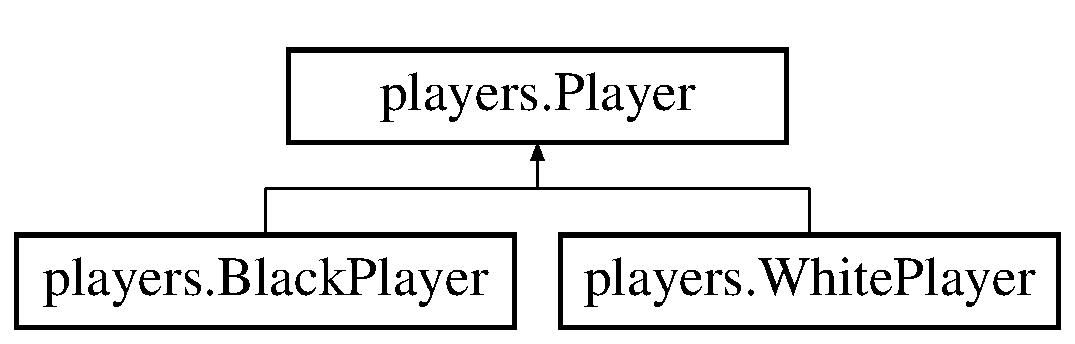
\includegraphics[height=2.000000cm]{classplayers_1_1_player}
\end{center}
\end{figure}
\subsection*{Public Member Functions}
\begin{DoxyCompactItemize}
\item 
\mbox{\Hypertarget{classplayers_1_1_player_ab00ac82acff3bd9f2f2c3a16f8f642ba}\label{classplayers_1_1_player_ab00ac82acff3bd9f2f2c3a16f8f642ba}} 
{\bfseries Player} (\mbox{\hyperlink{classgameboard_1_1_game_board}{Game\+Board}} board)
\item 
boolean \mbox{\hyperlink{classplayers_1_1_player_ad9049a1cec91bf5214100286f984cdaa}{move\+Piece}} (\mbox{\hyperlink{classpieces_1_1_move}{Move}} move)
\item 
boolean \mbox{\hyperlink{classplayers_1_1_player_a410730e0aede2a7253250ac892fc02e7}{has\+Lost}} ()
\item 
boolean \mbox{\hyperlink{classplayers_1_1_player_a5dc5f954097bc57cb2b1a63e1d32d00e}{is\+In\+Checkmate}} ()
\item 
boolean \mbox{\hyperlink{classplayers_1_1_player_ad7d20950f08db802354df71058addc8f}{is\+In\+Stalemate}} ()
\item 
\mbox{\Hypertarget{classplayers_1_1_player_a591346f361d949a7bbd825a4d764597e}\label{classplayers_1_1_player_a591346f361d949a7bbd825a4d764597e}} 
void {\bfseries restart} (\mbox{\hyperlink{classgameboard_1_1_game_board}{Game\+Board}} board)
\item 
\mbox{\Hypertarget{classplayers_1_1_player_a8461737a9f089305a750d4ef19992007}\label{classplayers_1_1_player_a8461737a9f089305a750d4ef19992007}} 
void {\bfseries add\+Score} ()
\item 
\mbox{\Hypertarget{classplayers_1_1_player_adb7c0bb6e8c72d9e16c333ef9e389ca2}\label{classplayers_1_1_player_adb7c0bb6e8c72d9e16c333ef9e389ca2}} 
int {\bfseries get\+Score} ()
\item 
abstract \mbox{\hyperlink{classpieces_1_1_piece}{Piece}} \mbox{\hyperlink{classplayers_1_1_player_a7a8d0f9a4ff654c5e1d936c8069d39ca}{get\+King}} ()
\item 
abstract Set$<$ \mbox{\hyperlink{classpieces_1_1_piece}{Piece}} $>$ \mbox{\hyperlink{classplayers_1_1_player_af1c0e492177ecbfa6bdc8e44b968ead3}{get\+Own\+Pieces}} ()
\item 
abstract Set$<$ \mbox{\hyperlink{classpieces_1_1_piece}{Piece}} $>$ \mbox{\hyperlink{classplayers_1_1_player_a71b0707e3607a9fdc2d8b94b49be1394}{get\+Opponent\+Pieces}} ()
\item 
abstract \mbox{\hyperlink{enumpieces_1_1_piece_1_1_piece_color}{Piece\+Color}} \mbox{\hyperlink{classplayers_1_1_player_a806f2042576092dced6bf5b9600f7763}{get\+Color}} ()
\end{DoxyCompactItemize}
\subsection*{Protected Attributes}
\begin{DoxyCompactItemize}
\item 
\mbox{\Hypertarget{classplayers_1_1_player_a1dd0db71975939835fe192a4062164fe}\label{classplayers_1_1_player_a1dd0db71975939835fe192a4062164fe}} 
\mbox{\hyperlink{classgameboard_1_1_game_board}{Game\+Board}} {\bfseries board}
\end{DoxyCompactItemize}


\subsection{Detailed Description}
Represents a player of the chess game Created by Siyang\+Liu on 2018/2/2. 

\subsection{Member Function Documentation}
\mbox{\Hypertarget{classplayers_1_1_player_a806f2042576092dced6bf5b9600f7763}\label{classplayers_1_1_player_a806f2042576092dced6bf5b9600f7763}} 
\index{players\+::\+Player@{players\+::\+Player}!get\+Color@{get\+Color}}
\index{get\+Color@{get\+Color}!players\+::\+Player@{players\+::\+Player}}
\subsubsection{\texorpdfstring{get\+Color()}{getColor()}}
{\footnotesize\ttfamily abstract \mbox{\hyperlink{enumpieces_1_1_piece_1_1_piece_color}{Piece\+Color}} players.\+Player.\+get\+Color (\begin{DoxyParamCaption}{ }\end{DoxyParamCaption})\hspace{0.3cm}{\ttfamily [abstract]}}

gets the color of the piece played by the player \mbox{\Hypertarget{classplayers_1_1_player_a7a8d0f9a4ff654c5e1d936c8069d39ca}\label{classplayers_1_1_player_a7a8d0f9a4ff654c5e1d936c8069d39ca}} 
\index{players\+::\+Player@{players\+::\+Player}!get\+King@{get\+King}}
\index{get\+King@{get\+King}!players\+::\+Player@{players\+::\+Player}}
\subsubsection{\texorpdfstring{get\+King()}{getKing()}}
{\footnotesize\ttfamily abstract \mbox{\hyperlink{classpieces_1_1_piece}{Piece}} players.\+Player.\+get\+King (\begin{DoxyParamCaption}{ }\end{DoxyParamCaption})\hspace{0.3cm}{\ttfamily [abstract]}}

gets the king of the player \mbox{\Hypertarget{classplayers_1_1_player_a71b0707e3607a9fdc2d8b94b49be1394}\label{classplayers_1_1_player_a71b0707e3607a9fdc2d8b94b49be1394}} 
\index{players\+::\+Player@{players\+::\+Player}!get\+Opponent\+Pieces@{get\+Opponent\+Pieces}}
\index{get\+Opponent\+Pieces@{get\+Opponent\+Pieces}!players\+::\+Player@{players\+::\+Player}}
\subsubsection{\texorpdfstring{get\+Opponent\+Pieces()}{getOpponentPieces()}}
{\footnotesize\ttfamily abstract Set$<$\mbox{\hyperlink{classpieces_1_1_piece}{Piece}}$>$ players.\+Player.\+get\+Opponent\+Pieces (\begin{DoxyParamCaption}{ }\end{DoxyParamCaption})\hspace{0.3cm}{\ttfamily [abstract]}}

gets the set of alive pieces of the opponent player \mbox{\Hypertarget{classplayers_1_1_player_af1c0e492177ecbfa6bdc8e44b968ead3}\label{classplayers_1_1_player_af1c0e492177ecbfa6bdc8e44b968ead3}} 
\index{players\+::\+Player@{players\+::\+Player}!get\+Own\+Pieces@{get\+Own\+Pieces}}
\index{get\+Own\+Pieces@{get\+Own\+Pieces}!players\+::\+Player@{players\+::\+Player}}
\subsubsection{\texorpdfstring{get\+Own\+Pieces()}{getOwnPieces()}}
{\footnotesize\ttfamily abstract Set$<$\mbox{\hyperlink{classpieces_1_1_piece}{Piece}}$>$ players.\+Player.\+get\+Own\+Pieces (\begin{DoxyParamCaption}{ }\end{DoxyParamCaption})\hspace{0.3cm}{\ttfamily [abstract]}}

gets the set of alive pieces of the player \mbox{\Hypertarget{classplayers_1_1_player_a410730e0aede2a7253250ac892fc02e7}\label{classplayers_1_1_player_a410730e0aede2a7253250ac892fc02e7}} 
\index{players\+::\+Player@{players\+::\+Player}!has\+Lost@{has\+Lost}}
\index{has\+Lost@{has\+Lost}!players\+::\+Player@{players\+::\+Player}}
\subsubsection{\texorpdfstring{has\+Lost()}{hasLost()}}
{\footnotesize\ttfamily boolean players.\+Player.\+has\+Lost (\begin{DoxyParamCaption}{ }\end{DoxyParamCaption})}

Checks if the player has lost the game \mbox{\Hypertarget{classplayers_1_1_player_a5dc5f954097bc57cb2b1a63e1d32d00e}\label{classplayers_1_1_player_a5dc5f954097bc57cb2b1a63e1d32d00e}} 
\index{players\+::\+Player@{players\+::\+Player}!is\+In\+Checkmate@{is\+In\+Checkmate}}
\index{is\+In\+Checkmate@{is\+In\+Checkmate}!players\+::\+Player@{players\+::\+Player}}
\subsubsection{\texorpdfstring{is\+In\+Checkmate()}{isInCheckmate()}}
{\footnotesize\ttfamily boolean players.\+Player.\+is\+In\+Checkmate (\begin{DoxyParamCaption}{ }\end{DoxyParamCaption})}

Checks if the player is in checkmate \mbox{\Hypertarget{classplayers_1_1_player_ad7d20950f08db802354df71058addc8f}\label{classplayers_1_1_player_ad7d20950f08db802354df71058addc8f}} 
\index{players\+::\+Player@{players\+::\+Player}!is\+In\+Stalemate@{is\+In\+Stalemate}}
\index{is\+In\+Stalemate@{is\+In\+Stalemate}!players\+::\+Player@{players\+::\+Player}}
\subsubsection{\texorpdfstring{is\+In\+Stalemate()}{isInStalemate()}}
{\footnotesize\ttfamily boolean players.\+Player.\+is\+In\+Stalemate (\begin{DoxyParamCaption}{ }\end{DoxyParamCaption})}

Checks if the player is in stalemate \mbox{\Hypertarget{classplayers_1_1_player_ad9049a1cec91bf5214100286f984cdaa}\label{classplayers_1_1_player_ad9049a1cec91bf5214100286f984cdaa}} 
\index{players\+::\+Player@{players\+::\+Player}!move\+Piece@{move\+Piece}}
\index{move\+Piece@{move\+Piece}!players\+::\+Player@{players\+::\+Player}}
\subsubsection{\texorpdfstring{move\+Piece()}{movePiece()}}
{\footnotesize\ttfamily boolean players.\+Player.\+move\+Piece (\begin{DoxyParamCaption}\item[{\mbox{\hyperlink{classpieces_1_1_move}{Move}}}]{move }\end{DoxyParamCaption})}

Moves a piece of the player 
\begin{DoxyParams}{Parameters}
{\em move} & the move that the player want to execute (may not be valid) \\
\hline
\end{DoxyParams}
\begin{DoxyReturn}{Returns}
whether the move is successfully executed 
\end{DoxyReturn}


The documentation for this class was generated from the following file\+:\begin{DoxyCompactItemize}
\item 
src/players/Player.\+java\end{DoxyCompactItemize}

\hypertarget{classtest_1_1_player_test}{}\section{test.\+Player\+Test Class Reference}
\label{classtest_1_1_player_test}\index{test.\+Player\+Test@{test.\+Player\+Test}}
Inheritance diagram for test.\+Player\+Test\+:\begin{figure}[H]
\begin{center}
\leavevmode
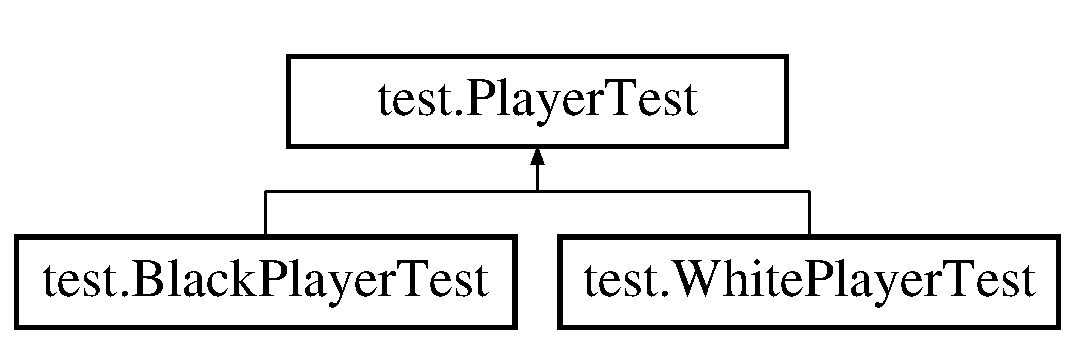
\includegraphics[height=2.000000cm]{classtest_1_1_player_test}
\end{center}
\end{figure}
\subsection*{Public Member Functions}
\begin{DoxyCompactItemize}
\item 
\mbox{\Hypertarget{classtest_1_1_player_test_a0c765458717b0bd798bf30917421e4c9}\label{classtest_1_1_player_test_a0c765458717b0bd798bf30917421e4c9}} 
void {\bfseries setup\+Board\+And\+Players} ()
\item 
void \mbox{\hyperlink{classtest_1_1_player_test_acc727d15c4b9047f5b91d30929b88cac}{move\+Piece1}} ()  throws Exception 
\item 
void \mbox{\hyperlink{classtest_1_1_player_test_a98a741ccef6e205a375db45f1292795a}{move\+Piece2}} ()  throws Exception 
\item 
void \mbox{\hyperlink{classtest_1_1_player_test_aab36d53fa06c66d4f9d8c091faebabc7}{move\+Piece3}} ()  throws Exception 
\item 
void \mbox{\hyperlink{classtest_1_1_player_test_ae63bfc10956604a272dfb769c713892f}{move\+Piece4}} ()  throws Exception 
\item 
void \mbox{\hyperlink{classtest_1_1_player_test_aad1ab6c518ab00c9bae07d229f07dd60}{is\+In\+Checkmate1}} ()  throws Exception 
\item 
void \mbox{\hyperlink{classtest_1_1_player_test_ac2a028bc355f58cd35398bd0c948403f}{is\+In\+Checkmate2}} ()  throws Exception 
\item 
void \mbox{\hyperlink{classtest_1_1_player_test_a0b1c927561968c583b282814f7940655}{is\+In\+Stalemate1}} ()  throws Exception 
\item 
\mbox{\Hypertarget{classtest_1_1_player_test_a19e8df2a5d16722d503b51fe8a72835c}\label{classtest_1_1_player_test_a19e8df2a5d16722d503b51fe8a72835c}} 
void {\bfseries is\+In\+Stalemate2} ()  throws Exception 
\item 
void \mbox{\hyperlink{classtest_1_1_player_test_a7d877a7e126bb1e49ba84ab606dc7fc6}{get\+King}} ()  throws Exception 
\item 
void \mbox{\hyperlink{classtest_1_1_player_test_a79edf065f06225fbd9d83323a2976b6c}{get\+Own\+Piece}} ()  throws Exception 
\item 
void \mbox{\hyperlink{classtest_1_1_player_test_a492f1c20801511404ba2245fb1706c96}{get\+Opponent\+Pieces}} ()  throws Exception
\end{DoxyCompactItemize}
\subsection*{Protected Member Functions}
\begin{DoxyCompactItemize}
\item 
abstract \mbox{\hyperlink{classplayers_1_1_player}{Player}} \mbox{\hyperlink{classtest_1_1_player_test_a8d7c124dab2eb1050aa1b96b2d6bb2eb}{get\+Concrete\+Self}} (\mbox{\hyperlink{classgameboard_1_1_game_board}{Game\+Board}} board)
\item 
abstract \mbox{\hyperlink{classplayers_1_1_player}{Player}} \mbox{\hyperlink{classtest_1_1_player_test_a8d1acf8417e1fd66430c01d318fee3ac}{get\+Concrete\+Opponent}} (\mbox{\hyperlink{classgameboard_1_1_game_board}{Game\+Board}} board)
\end{DoxyCompactItemize}
\subsection*{Protected Attributes}
\begin{DoxyCompactItemize}
\item 
\mbox{\Hypertarget{classtest_1_1_player_test_a6264044f63d7fae1dba6c3a1b3d76454}\label{classtest_1_1_player_test_a6264044f63d7fae1dba6c3a1b3d76454}} 
\mbox{\hyperlink{classgameboard_1_1_game_board}{Game\+Board}} {\bfseries board}
\end{DoxyCompactItemize}


\subsection{Detailed Description}
Test for the operations of a Player Created by Siyang\+Liu on 2018/2/4. 

\subsection{Member Function Documentation}
\mbox{\Hypertarget{classtest_1_1_player_test_a8d1acf8417e1fd66430c01d318fee3ac}\label{classtest_1_1_player_test_a8d1acf8417e1fd66430c01d318fee3ac}} 
\index{test\+::\+Player\+Test@{test\+::\+Player\+Test}!get\+Concrete\+Opponent@{get\+Concrete\+Opponent}}
\index{get\+Concrete\+Opponent@{get\+Concrete\+Opponent}!test\+::\+Player\+Test@{test\+::\+Player\+Test}}
\subsubsection{\texorpdfstring{get\+Concrete\+Opponent()}{getConcreteOpponent()}}
{\footnotesize\ttfamily abstract \mbox{\hyperlink{classplayers_1_1_player}{Player}} test.\+Player\+Test.\+get\+Concrete\+Opponent (\begin{DoxyParamCaption}\item[{\mbox{\hyperlink{classgameboard_1_1_game_board}{Game\+Board}}}]{board }\end{DoxyParamCaption})\hspace{0.3cm}{\ttfamily [abstract]}, {\ttfamily [protected]}}

Construct a concrete opponent Player \mbox{\Hypertarget{classtest_1_1_player_test_a8d7c124dab2eb1050aa1b96b2d6bb2eb}\label{classtest_1_1_player_test_a8d7c124dab2eb1050aa1b96b2d6bb2eb}} 
\index{test\+::\+Player\+Test@{test\+::\+Player\+Test}!get\+Concrete\+Self@{get\+Concrete\+Self}}
\index{get\+Concrete\+Self@{get\+Concrete\+Self}!test\+::\+Player\+Test@{test\+::\+Player\+Test}}
\subsubsection{\texorpdfstring{get\+Concrete\+Self()}{getConcreteSelf()}}
{\footnotesize\ttfamily abstract \mbox{\hyperlink{classplayers_1_1_player}{Player}} test.\+Player\+Test.\+get\+Concrete\+Self (\begin{DoxyParamCaption}\item[{\mbox{\hyperlink{classgameboard_1_1_game_board}{Game\+Board}}}]{board }\end{DoxyParamCaption})\hspace{0.3cm}{\ttfamily [abstract]}, {\ttfamily [protected]}}

Construct a concrete Player \mbox{\Hypertarget{classtest_1_1_player_test_a7d877a7e126bb1e49ba84ab606dc7fc6}\label{classtest_1_1_player_test_a7d877a7e126bb1e49ba84ab606dc7fc6}} 
\index{test\+::\+Player\+Test@{test\+::\+Player\+Test}!get\+King@{get\+King}}
\index{get\+King@{get\+King}!test\+::\+Player\+Test@{test\+::\+Player\+Test}}
\subsubsection{\texorpdfstring{get\+King()}{getKing()}}
{\footnotesize\ttfamily void test.\+Player\+Test.\+get\+King (\begin{DoxyParamCaption}{ }\end{DoxyParamCaption}) throws Exception}

Test if the king can be get \mbox{\Hypertarget{classtest_1_1_player_test_a492f1c20801511404ba2245fb1706c96}\label{classtest_1_1_player_test_a492f1c20801511404ba2245fb1706c96}} 
\index{test\+::\+Player\+Test@{test\+::\+Player\+Test}!get\+Opponent\+Pieces@{get\+Opponent\+Pieces}}
\index{get\+Opponent\+Pieces@{get\+Opponent\+Pieces}!test\+::\+Player\+Test@{test\+::\+Player\+Test}}
\subsubsection{\texorpdfstring{get\+Opponent\+Pieces()}{getOpponentPieces()}}
{\footnotesize\ttfamily void test.\+Player\+Test.\+get\+Opponent\+Pieces (\begin{DoxyParamCaption}{ }\end{DoxyParamCaption}) throws Exception}

Test if all opponent\textquotesingle{}s pieces can be get correctly \mbox{\Hypertarget{classtest_1_1_player_test_a79edf065f06225fbd9d83323a2976b6c}\label{classtest_1_1_player_test_a79edf065f06225fbd9d83323a2976b6c}} 
\index{test\+::\+Player\+Test@{test\+::\+Player\+Test}!get\+Own\+Piece@{get\+Own\+Piece}}
\index{get\+Own\+Piece@{get\+Own\+Piece}!test\+::\+Player\+Test@{test\+::\+Player\+Test}}
\subsubsection{\texorpdfstring{get\+Own\+Piece()}{getOwnPiece()}}
{\footnotesize\ttfamily void test.\+Player\+Test.\+get\+Own\+Piece (\begin{DoxyParamCaption}{ }\end{DoxyParamCaption}) throws Exception}

Test if all own pieces can be get correctly \mbox{\Hypertarget{classtest_1_1_player_test_aad1ab6c518ab00c9bae07d229f07dd60}\label{classtest_1_1_player_test_aad1ab6c518ab00c9bae07d229f07dd60}} 
\index{test\+::\+Player\+Test@{test\+::\+Player\+Test}!is\+In\+Checkmate1@{is\+In\+Checkmate1}}
\index{is\+In\+Checkmate1@{is\+In\+Checkmate1}!test\+::\+Player\+Test@{test\+::\+Player\+Test}}
\subsubsection{\texorpdfstring{is\+In\+Checkmate1()}{isInCheckmate1()}}
{\footnotesize\ttfamily void test.\+Player\+Test.\+is\+In\+Checkmate1 (\begin{DoxyParamCaption}{ }\end{DoxyParamCaption}) throws Exception}

Test if a checkmate can be detected \mbox{\Hypertarget{classtest_1_1_player_test_ac2a028bc355f58cd35398bd0c948403f}\label{classtest_1_1_player_test_ac2a028bc355f58cd35398bd0c948403f}} 
\index{test\+::\+Player\+Test@{test\+::\+Player\+Test}!is\+In\+Checkmate2@{is\+In\+Checkmate2}}
\index{is\+In\+Checkmate2@{is\+In\+Checkmate2}!test\+::\+Player\+Test@{test\+::\+Player\+Test}}
\subsubsection{\texorpdfstring{is\+In\+Checkmate2()}{isInCheckmate2()}}
{\footnotesize\ttfamily void test.\+Player\+Test.\+is\+In\+Checkmate2 (\begin{DoxyParamCaption}{ }\end{DoxyParamCaption}) throws Exception}

Test if a checkmate can be detected \mbox{\Hypertarget{classtest_1_1_player_test_a0b1c927561968c583b282814f7940655}\label{classtest_1_1_player_test_a0b1c927561968c583b282814f7940655}} 
\index{test\+::\+Player\+Test@{test\+::\+Player\+Test}!is\+In\+Stalemate1@{is\+In\+Stalemate1}}
\index{is\+In\+Stalemate1@{is\+In\+Stalemate1}!test\+::\+Player\+Test@{test\+::\+Player\+Test}}
\subsubsection{\texorpdfstring{is\+In\+Stalemate1()}{isInStalemate1()}}
{\footnotesize\ttfamily void test.\+Player\+Test.\+is\+In\+Stalemate1 (\begin{DoxyParamCaption}{ }\end{DoxyParamCaption}) throws Exception}

Test if a stalemate can be detected \mbox{\Hypertarget{classtest_1_1_player_test_acc727d15c4b9047f5b91d30929b88cac}\label{classtest_1_1_player_test_acc727d15c4b9047f5b91d30929b88cac}} 
\index{test\+::\+Player\+Test@{test\+::\+Player\+Test}!move\+Piece1@{move\+Piece1}}
\index{move\+Piece1@{move\+Piece1}!test\+::\+Player\+Test@{test\+::\+Player\+Test}}
\subsubsection{\texorpdfstring{move\+Piece1()}{movePiece1()}}
{\footnotesize\ttfamily void test.\+Player\+Test.\+move\+Piece1 (\begin{DoxyParamCaption}{ }\end{DoxyParamCaption}) throws Exception}

Checks if moves of a pawn can be executed correctly first move and non-\/first move are executed \mbox{\Hypertarget{classtest_1_1_player_test_a98a741ccef6e205a375db45f1292795a}\label{classtest_1_1_player_test_a98a741ccef6e205a375db45f1292795a}} 
\index{test\+::\+Player\+Test@{test\+::\+Player\+Test}!move\+Piece2@{move\+Piece2}}
\index{move\+Piece2@{move\+Piece2}!test\+::\+Player\+Test@{test\+::\+Player\+Test}}
\subsubsection{\texorpdfstring{move\+Piece2()}{movePiece2()}}
{\footnotesize\ttfamily void test.\+Player\+Test.\+move\+Piece2 (\begin{DoxyParamCaption}{ }\end{DoxyParamCaption}) throws Exception}

Checks if moves can be executed correctly \mbox{\Hypertarget{classtest_1_1_player_test_aab36d53fa06c66d4f9d8c091faebabc7}\label{classtest_1_1_player_test_aab36d53fa06c66d4f9d8c091faebabc7}} 
\index{test\+::\+Player\+Test@{test\+::\+Player\+Test}!move\+Piece3@{move\+Piece3}}
\index{move\+Piece3@{move\+Piece3}!test\+::\+Player\+Test@{test\+::\+Player\+Test}}
\subsubsection{\texorpdfstring{move\+Piece3()}{movePiece3()}}
{\footnotesize\ttfamily void test.\+Player\+Test.\+move\+Piece3 (\begin{DoxyParamCaption}{ }\end{DoxyParamCaption}) throws Exception}

Checks if moves failure can be detected with occupied destination squares \mbox{\Hypertarget{classtest_1_1_player_test_ae63bfc10956604a272dfb769c713892f}\label{classtest_1_1_player_test_ae63bfc10956604a272dfb769c713892f}} 
\index{test\+::\+Player\+Test@{test\+::\+Player\+Test}!move\+Piece4@{move\+Piece4}}
\index{move\+Piece4@{move\+Piece4}!test\+::\+Player\+Test@{test\+::\+Player\+Test}}
\subsubsection{\texorpdfstring{move\+Piece4()}{movePiece4()}}
{\footnotesize\ttfamily void test.\+Player\+Test.\+move\+Piece4 (\begin{DoxyParamCaption}{ }\end{DoxyParamCaption}) throws Exception}

Checks if moves failure can be detected when it is illegal

Checks if moves can be executed correctly 

The documentation for this class was generated from the following file\+:\begin{DoxyCompactItemize}
\item 
src/test/Player\+Test.\+java\end{DoxyCompactItemize}

\hypertarget{classpieces_1_1_queen}{}\section{pieces.\+Queen Class Reference}
\label{classpieces_1_1_queen}\index{pieces.\+Queen@{pieces.\+Queen}}
Inheritance diagram for pieces.\+Queen\+:\begin{figure}[H]
\begin{center}
\leavevmode
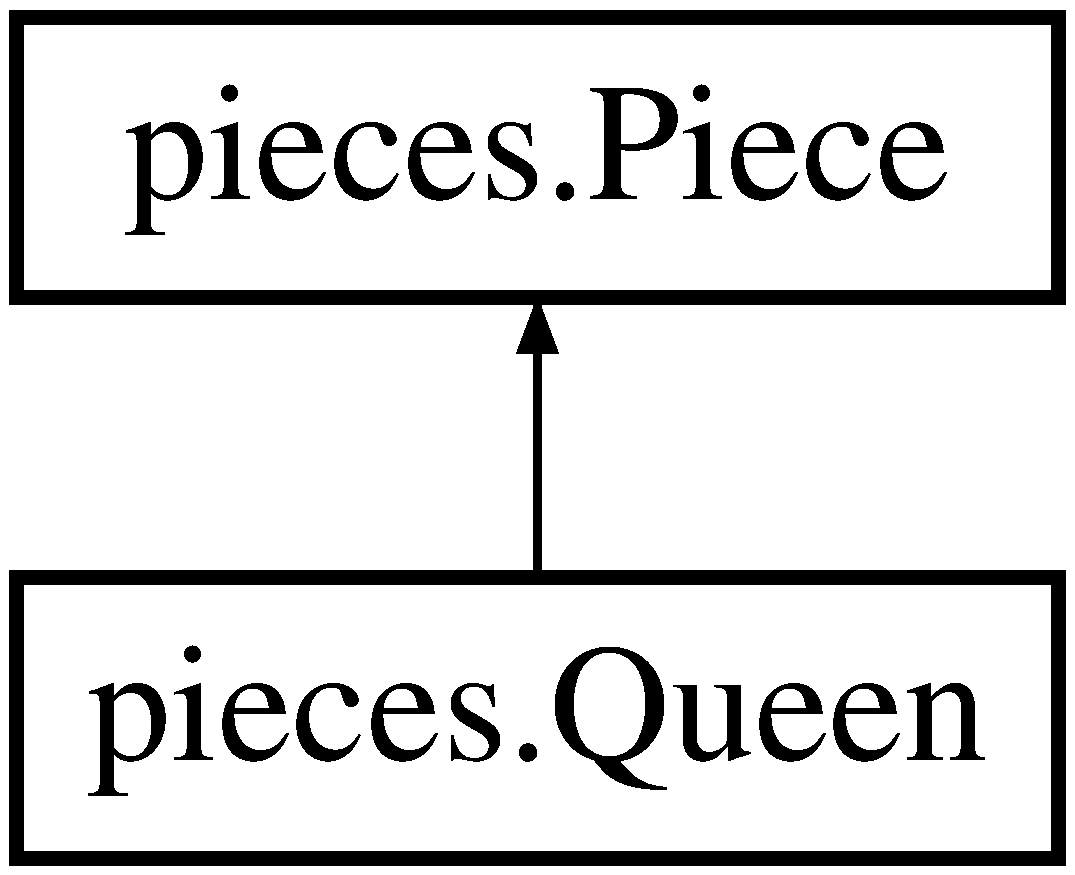
\includegraphics[height=2.000000cm]{classpieces_1_1_queen}
\end{center}
\end{figure}
\subsection*{Public Member Functions}
\begin{DoxyCompactItemize}
\item 
\mbox{\Hypertarget{classpieces_1_1_queen_a94fac9d3eb7ef6ef47a0cbbe236ccc69}\label{classpieces_1_1_queen_a94fac9d3eb7ef6ef47a0cbbe236ccc69}} 
{\bfseries Queen} (\mbox{\hyperlink{enumpieces_1_1_piece_1_1_piece_color}{Piece\+Color}} piece\+Color, int coordinate\+Row, int coordinate\+Col)
\item 
\mbox{\Hypertarget{classpieces_1_1_queen_a915eee4d0da44bc2a43b28ba4a971eec}\label{classpieces_1_1_queen_a915eee4d0da44bc2a43b28ba4a971eec}} 
List$<$ \mbox{\hyperlink{classpieces_1_1_move}{Move}} $>$ {\bfseries compute\+Valid\+Moves} (\mbox{\hyperlink{classgameboard_1_1_game_board}{Game\+Board}} board)
\item 
\mbox{\Hypertarget{classpieces_1_1_queen_a75e77de99a0da6a3422f918da86e4de4}\label{classpieces_1_1_queen_a75e77de99a0da6a3422f918da86e4de4}} 
String {\bfseries get\+String} ()
\end{DoxyCompactItemize}
\subsection*{Additional Inherited Members}


\subsection{Detailed Description}
Represents a \mbox{\hyperlink{classpieces_1_1_queen}{Queen}} piece of the chess game Created by Siyang\+Liu on 2018/2/2. 

The documentation for this class was generated from the following file\+:\begin{DoxyCompactItemize}
\item 
src/pieces/Queen.\+java\end{DoxyCompactItemize}

\hypertarget{classtest_1_1_queen_test}{}\section{test.\+Queen\+Test Class Reference}
\label{classtest_1_1_queen_test}\index{test.\+Queen\+Test@{test.\+Queen\+Test}}
Inheritance diagram for test.\+Queen\+Test\+:\begin{figure}[H]
\begin{center}
\leavevmode
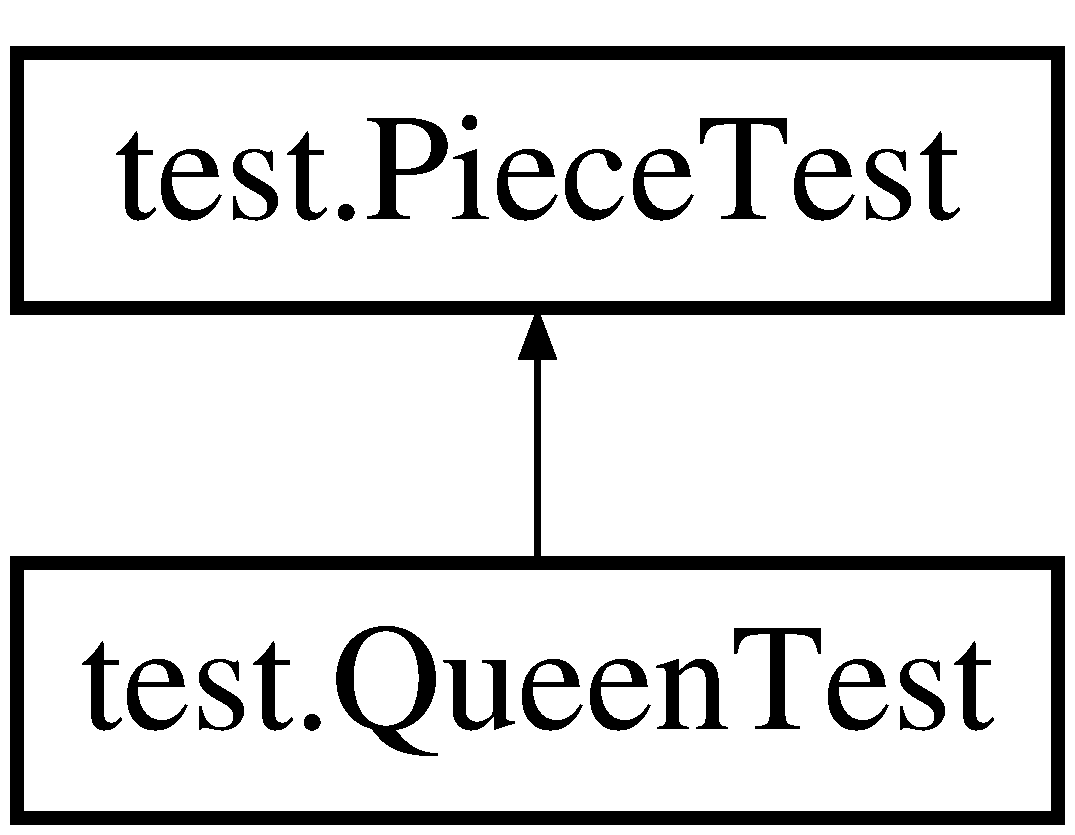
\includegraphics[height=2.000000cm]{classtest_1_1_queen_test}
\end{center}
\end{figure}
\subsection*{Public Member Functions}
\begin{DoxyCompactItemize}
\item 
\mbox{\Hypertarget{classtest_1_1_queen_test_ae382115ee724469b7c5f4200c534ef19}\label{classtest_1_1_queen_test_ae382115ee724469b7c5f4200c534ef19}} 
void {\bfseries Valid\+Constructor2} ()  throws Exception 
\item 
\mbox{\Hypertarget{classtest_1_1_queen_test_a6ec00eab5072d465ffd954787d6e8dd3}\label{classtest_1_1_queen_test_a6ec00eab5072d465ffd954787d6e8dd3}} 
void {\bfseries compute\+Valid\+Moves} ()  throws Exception 
\end{DoxyCompactItemize}
\subsection*{Protected Member Functions}
\begin{DoxyCompactItemize}
\item 
\mbox{\Hypertarget{classtest_1_1_queen_test_acb7901fbd2a81c67c739f72bbfe98f6d}\label{classtest_1_1_queen_test_acb7901fbd2a81c67c739f72bbfe98f6d}} 
\mbox{\hyperlink{classpieces_1_1_piece}{Piece}} {\bfseries get\+Concrete} (\mbox{\hyperlink{enumpieces_1_1_piece_1_1_piece_color}{Piece.\+Piece\+Color}} piece\+Color, int coordinate\+Row, int coordinate\+Col)
\end{DoxyCompactItemize}
\subsection*{Additional Inherited Members}


\subsection{Detailed Description}
Test for the operations of a Queen Created by Siyang\+Liu on 2018/2/4. 

The documentation for this class was generated from the following file\+:\begin{DoxyCompactItemize}
\item 
src/test/Queen\+Test.\+java\end{DoxyCompactItemize}

\hypertarget{classpieces_1_1_rook}{}\section{pieces.\+Rook Class Reference}
\label{classpieces_1_1_rook}\index{pieces.\+Rook@{pieces.\+Rook}}
Inheritance diagram for pieces.\+Rook\+:\begin{figure}[H]
\begin{center}
\leavevmode
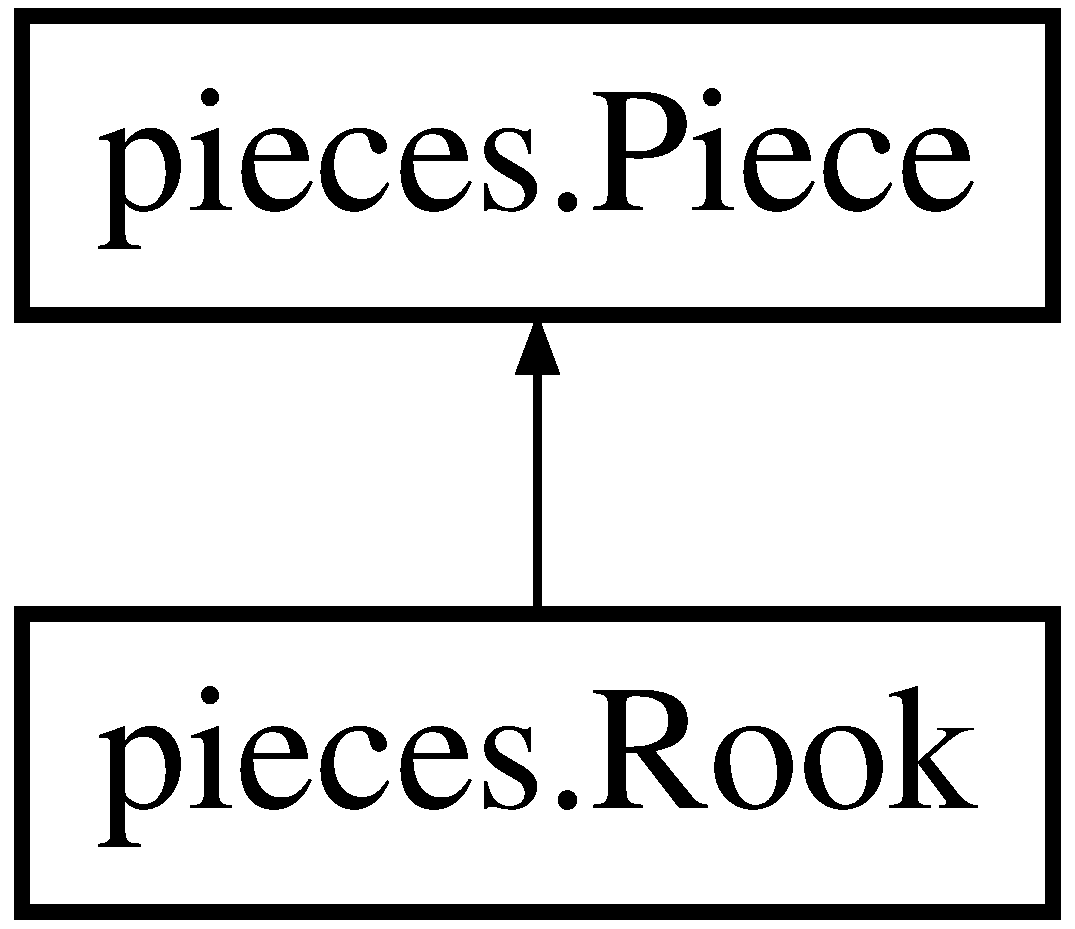
\includegraphics[height=2.000000cm]{classpieces_1_1_rook}
\end{center}
\end{figure}
\subsection*{Public Member Functions}
\begin{DoxyCompactItemize}
\item 
\mbox{\Hypertarget{classpieces_1_1_rook_a3bdcb3d2152c8b9370ee0d88a98e005d}\label{classpieces_1_1_rook_a3bdcb3d2152c8b9370ee0d88a98e005d}} 
{\bfseries Rook} (\mbox{\hyperlink{enumpieces_1_1_piece_1_1_piece_color}{Piece\+Color}} piece\+Color, int coordinate\+Row, int coordinate\+Col)
\item 
\mbox{\Hypertarget{classpieces_1_1_rook_ac41fa0491a74087d1b2309236fb755cc}\label{classpieces_1_1_rook_ac41fa0491a74087d1b2309236fb755cc}} 
List$<$ \mbox{\hyperlink{classpieces_1_1_move}{Move}} $>$ {\bfseries compute\+Valid\+Moves} (\mbox{\hyperlink{classgameboard_1_1_game_board}{Game\+Board}} board)
\item 
\mbox{\Hypertarget{classpieces_1_1_rook_a686b53b7dbb0dee50cd5a2e4557a8cb0}\label{classpieces_1_1_rook_a686b53b7dbb0dee50cd5a2e4557a8cb0}} 
String {\bfseries get\+String} ()
\end{DoxyCompactItemize}
\subsection*{Additional Inherited Members}


\subsection{Detailed Description}
Represents a \mbox{\hyperlink{classpieces_1_1_rook}{Rook}} piece of the chess game Created by Siyang\+Liu on 2018/2/2. 

The documentation for this class was generated from the following file\+:\begin{DoxyCompactItemize}
\item 
src/pieces/Rook.\+java\end{DoxyCompactItemize}

\hypertarget{classtest_1_1_rook_test}{}\section{test.\+Rook\+Test Class Reference}
\label{classtest_1_1_rook_test}\index{test.\+Rook\+Test@{test.\+Rook\+Test}}
Inheritance diagram for test.\+Rook\+Test\+:\begin{figure}[H]
\begin{center}
\leavevmode
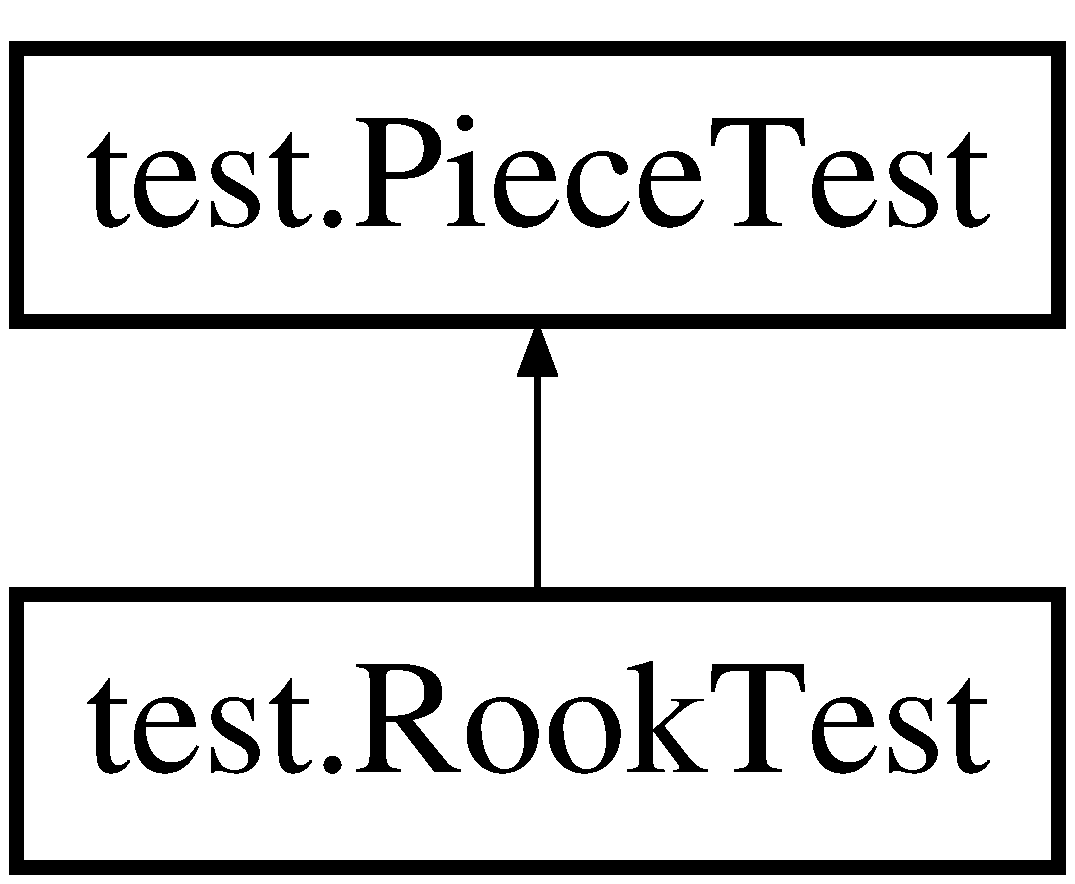
\includegraphics[height=2.000000cm]{classtest_1_1_rook_test}
\end{center}
\end{figure}
\subsection*{Public Member Functions}
\begin{DoxyCompactItemize}
\item 
\mbox{\Hypertarget{classtest_1_1_rook_test_a38216b286eae6ff708b28298ad322bae}\label{classtest_1_1_rook_test_a38216b286eae6ff708b28298ad322bae}} 
void {\bfseries Valid\+Constructor2} ()  throws Exception 
\item 
\mbox{\Hypertarget{classtest_1_1_rook_test_ae43390f12cb6c38b537231331b78e82a}\label{classtest_1_1_rook_test_ae43390f12cb6c38b537231331b78e82a}} 
void {\bfseries compute\+Valid\+Moves} ()  throws Exception 
\end{DoxyCompactItemize}
\subsection*{Protected Member Functions}
\begin{DoxyCompactItemize}
\item 
\mbox{\Hypertarget{classtest_1_1_rook_test_ae20996d61c928faa97e7aeb11119ec68}\label{classtest_1_1_rook_test_ae20996d61c928faa97e7aeb11119ec68}} 
\mbox{\hyperlink{classpieces_1_1_piece}{Piece}} {\bfseries get\+Concrete} (\mbox{\hyperlink{enumpieces_1_1_piece_1_1_piece_color}{Piece.\+Piece\+Color}} piece\+Color, int coordinate\+Row, int coordinate\+Col)
\end{DoxyCompactItemize}
\subsection*{Additional Inherited Members}


\subsection{Detailed Description}
Test for the operations of a Rook Created by Siyang\+Liu on 2018/2/4. 

The documentation for this class was generated from the following file\+:\begin{DoxyCompactItemize}
\item 
src/test/Rook\+Test.\+java\end{DoxyCompactItemize}

\hypertarget{classgui_1_1_view_1_1_score_panel}{}\section{gui.\+View.\+Score\+Panel Class Reference}
\label{classgui_1_1_view_1_1_score_panel}\index{gui.\+View.\+Score\+Panel@{gui.\+View.\+Score\+Panel}}
Inheritance diagram for gui.\+View.\+Score\+Panel\+:\begin{figure}[H]
\begin{center}
\leavevmode
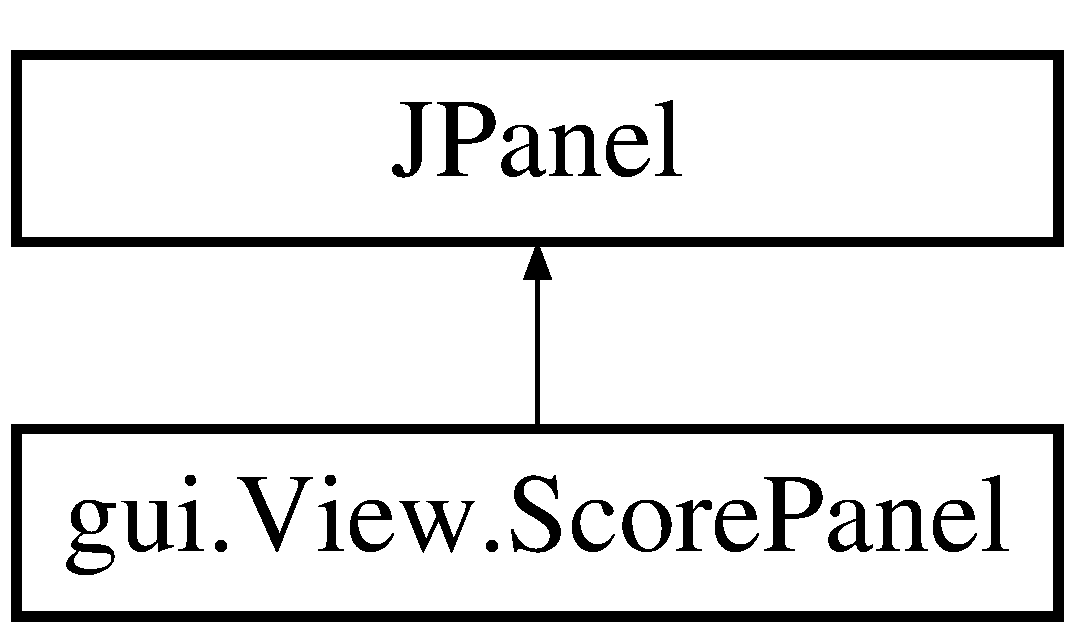
\includegraphics[height=2.000000cm]{classgui_1_1_view_1_1_score_panel}
\end{center}
\end{figure}
\subsection*{Public Member Functions}
\begin{DoxyCompactItemize}
\item 
\mbox{\hyperlink{enumpieces_1_1_piece_1_1_piece_color}{Piece\+Color}} \mbox{\hyperlink{classgui_1_1_view_1_1_score_panel_a162bd408d798b9d65253147b83d9feae}{get\+Color}} ()
\item 
void \mbox{\hyperlink{classgui_1_1_view_1_1_score_panel_a3dd245187918d98e62c6059980528cd7}{set\+Name}} (String name)
\end{DoxyCompactItemize}


\subsection{Detailed Description}
A Panel with the profile, name and score of a player 

\subsection{Member Function Documentation}
\mbox{\Hypertarget{classgui_1_1_view_1_1_score_panel_a162bd408d798b9d65253147b83d9feae}\label{classgui_1_1_view_1_1_score_panel_a162bd408d798b9d65253147b83d9feae}} 
\index{gui\+::\+View\+::\+Score\+Panel@{gui\+::\+View\+::\+Score\+Panel}!get\+Color@{get\+Color}}
\index{get\+Color@{get\+Color}!gui\+::\+View\+::\+Score\+Panel@{gui\+::\+View\+::\+Score\+Panel}}
\subsubsection{\texorpdfstring{get\+Color()}{getColor()}}
{\footnotesize\ttfamily \mbox{\hyperlink{enumpieces_1_1_piece_1_1_piece_color}{Piece\+Color}} gui.\+View.\+Score\+Panel.\+get\+Color (\begin{DoxyParamCaption}{ }\end{DoxyParamCaption})}

get the owner of the score panel \mbox{\Hypertarget{classgui_1_1_view_1_1_score_panel_a3dd245187918d98e62c6059980528cd7}\label{classgui_1_1_view_1_1_score_panel_a3dd245187918d98e62c6059980528cd7}} 
\index{gui\+::\+View\+::\+Score\+Panel@{gui\+::\+View\+::\+Score\+Panel}!set\+Name@{set\+Name}}
\index{set\+Name@{set\+Name}!gui\+::\+View\+::\+Score\+Panel@{gui\+::\+View\+::\+Score\+Panel}}
\subsubsection{\texorpdfstring{set\+Name()}{setName()}}
{\footnotesize\ttfamily void gui.\+View.\+Score\+Panel.\+set\+Name (\begin{DoxyParamCaption}\item[{String}]{name }\end{DoxyParamCaption})}

Sets the name of the player to display it in the score panel 
\begin{DoxyParams}{Parameters}
{\em name} & \\
\hline
\end{DoxyParams}


The documentation for this class was generated from the following file\+:\begin{DoxyCompactItemize}
\item 
src/gui/View.\+java\end{DoxyCompactItemize}

\hypertarget{classgameboard_1_1_square}{}\section{gameboard.\+Square Class Reference}
\label{classgameboard_1_1_square}\index{gameboard.\+Square@{gameboard.\+Square}}
\subsection*{Public Member Functions}
\begin{DoxyCompactItemize}
\item 
\mbox{\Hypertarget{classgameboard_1_1_square_a4ca76f3829c4ddbc95a4bfad30896338}\label{classgameboard_1_1_square_a4ca76f3829c4ddbc95a4bfad30896338}} 
{\bfseries Square} (int row\+Index, int col\+Index, \mbox{\hyperlink{classpieces_1_1_piece}{Piece}} piece)
\item 
boolean \mbox{\hyperlink{classgameboard_1_1_square_a0ad09157aca37441420daf27de6a2f63}{has\+Piece}} ()
\item 
\mbox{\hyperlink{classpieces_1_1_piece}{Piece}} \mbox{\hyperlink{classgameboard_1_1_square_a7c261d1ec58046f8b580efe45e751382}{get\+Piece}} ()
\item 
int \mbox{\hyperlink{classgameboard_1_1_square_a45ee059f08475d6d83571857f8e8f6ae}{get\+Row\+Index}} ()
\item 
int \mbox{\hyperlink{classgameboard_1_1_square_a821e41d4a1343edd5804c280a032871d}{get\+Col\+Index}} ()
\item 
void \mbox{\hyperlink{classgameboard_1_1_square_abc200e09f6066535d09eab796688eabe}{set\+Empty}} ()
\item 
void \mbox{\hyperlink{classgameboard_1_1_square_ae3145cd4d46cf412624aef20c03b002b}{set\+Piece}} (\mbox{\hyperlink{classpieces_1_1_piece}{Piece}} piece)
\end{DoxyCompactItemize}


\subsection{Detailed Description}
Represents a single square in the game board Created by Siyang\+Liu on 2018/2/1. 

\subsection{Member Function Documentation}
\mbox{\Hypertarget{classgameboard_1_1_square_a821e41d4a1343edd5804c280a032871d}\label{classgameboard_1_1_square_a821e41d4a1343edd5804c280a032871d}} 
\index{gameboard\+::\+Square@{gameboard\+::\+Square}!get\+Col\+Index@{get\+Col\+Index}}
\index{get\+Col\+Index@{get\+Col\+Index}!gameboard\+::\+Square@{gameboard\+::\+Square}}
\subsubsection{\texorpdfstring{get\+Col\+Index()}{getColIndex()}}
{\footnotesize\ttfamily int gameboard.\+Square.\+get\+Col\+Index (\begin{DoxyParamCaption}{ }\end{DoxyParamCaption})}

Gets the column index of the square \mbox{\Hypertarget{classgameboard_1_1_square_a7c261d1ec58046f8b580efe45e751382}\label{classgameboard_1_1_square_a7c261d1ec58046f8b580efe45e751382}} 
\index{gameboard\+::\+Square@{gameboard\+::\+Square}!get\+Piece@{get\+Piece}}
\index{get\+Piece@{get\+Piece}!gameboard\+::\+Square@{gameboard\+::\+Square}}
\subsubsection{\texorpdfstring{get\+Piece()}{getPiece()}}
{\footnotesize\ttfamily \mbox{\hyperlink{classpieces_1_1_piece}{Piece}} gameboard.\+Square.\+get\+Piece (\begin{DoxyParamCaption}{ }\end{DoxyParamCaption})}

Gets the piece placed in the square \begin{DoxyReturn}{Returns}
null if no piece 
\end{DoxyReturn}
\mbox{\Hypertarget{classgameboard_1_1_square_a45ee059f08475d6d83571857f8e8f6ae}\label{classgameboard_1_1_square_a45ee059f08475d6d83571857f8e8f6ae}} 
\index{gameboard\+::\+Square@{gameboard\+::\+Square}!get\+Row\+Index@{get\+Row\+Index}}
\index{get\+Row\+Index@{get\+Row\+Index}!gameboard\+::\+Square@{gameboard\+::\+Square}}
\subsubsection{\texorpdfstring{get\+Row\+Index()}{getRowIndex()}}
{\footnotesize\ttfamily int gameboard.\+Square.\+get\+Row\+Index (\begin{DoxyParamCaption}{ }\end{DoxyParamCaption})}

Gets the row index of the square \mbox{\Hypertarget{classgameboard_1_1_square_a0ad09157aca37441420daf27de6a2f63}\label{classgameboard_1_1_square_a0ad09157aca37441420daf27de6a2f63}} 
\index{gameboard\+::\+Square@{gameboard\+::\+Square}!has\+Piece@{has\+Piece}}
\index{has\+Piece@{has\+Piece}!gameboard\+::\+Square@{gameboard\+::\+Square}}
\subsubsection{\texorpdfstring{has\+Piece()}{hasPiece()}}
{\footnotesize\ttfamily boolean gameboard.\+Square.\+has\+Piece (\begin{DoxyParamCaption}{ }\end{DoxyParamCaption})}

Checks if the square has a piece \mbox{\Hypertarget{classgameboard_1_1_square_abc200e09f6066535d09eab796688eabe}\label{classgameboard_1_1_square_abc200e09f6066535d09eab796688eabe}} 
\index{gameboard\+::\+Square@{gameboard\+::\+Square}!set\+Empty@{set\+Empty}}
\index{set\+Empty@{set\+Empty}!gameboard\+::\+Square@{gameboard\+::\+Square}}
\subsubsection{\texorpdfstring{set\+Empty()}{setEmpty()}}
{\footnotesize\ttfamily void gameboard.\+Square.\+set\+Empty (\begin{DoxyParamCaption}{ }\end{DoxyParamCaption})}

Removes the piece in the square \mbox{\Hypertarget{classgameboard_1_1_square_ae3145cd4d46cf412624aef20c03b002b}\label{classgameboard_1_1_square_ae3145cd4d46cf412624aef20c03b002b}} 
\index{gameboard\+::\+Square@{gameboard\+::\+Square}!set\+Piece@{set\+Piece}}
\index{set\+Piece@{set\+Piece}!gameboard\+::\+Square@{gameboard\+::\+Square}}
\subsubsection{\texorpdfstring{set\+Piece()}{setPiece()}}
{\footnotesize\ttfamily void gameboard.\+Square.\+set\+Piece (\begin{DoxyParamCaption}\item[{\mbox{\hyperlink{classpieces_1_1_piece}{Piece}}}]{piece }\end{DoxyParamCaption})}

Places the given piece in the square 

The documentation for this class was generated from the following file\+:\begin{DoxyCompactItemize}
\item 
src/gameboard/Square.\+java\end{DoxyCompactItemize}

\hypertarget{classgui_1_1_view_1_1_square_panel}{}\section{gui.\+View.\+Square\+Panel Class Reference}
\label{classgui_1_1_view_1_1_square_panel}\index{gui.\+View.\+Square\+Panel@{gui.\+View.\+Square\+Panel}}
Inheritance diagram for gui.\+View.\+Square\+Panel\+:\begin{figure}[H]
\begin{center}
\leavevmode
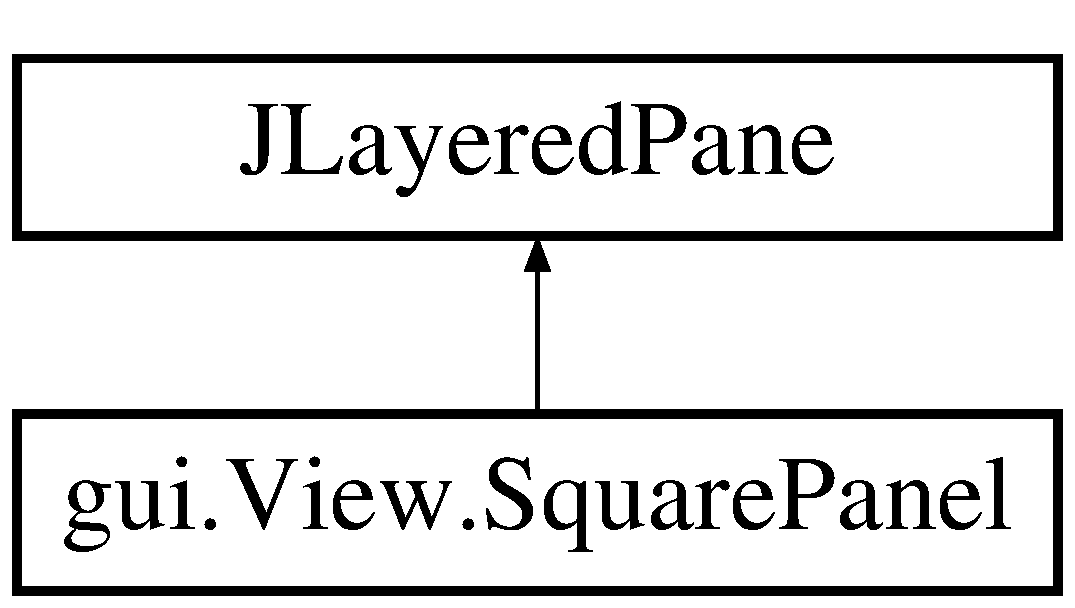
\includegraphics[height=2.000000cm]{classgui_1_1_view_1_1_square_panel}
\end{center}
\end{figure}
\subsection*{Public Member Functions}
\begin{DoxyCompactItemize}
\item 
int \mbox{[}$\,$\mbox{]} \mbox{\hyperlink{classgui_1_1_view_1_1_square_panel_a97328a4344b3c3e02319419dcdb3e7c5}{get\+Coordinates}} ()
\end{DoxyCompactItemize}


\subsection{Detailed Description}
A \mbox{\hyperlink{classgui_1_1_view_1_1_square_panel}{Square\+Panel}} is a J\+Panel which contains the components of each square in a chess board 

\subsection{Member Function Documentation}
\mbox{\Hypertarget{classgui_1_1_view_1_1_square_panel_a97328a4344b3c3e02319419dcdb3e7c5}\label{classgui_1_1_view_1_1_square_panel_a97328a4344b3c3e02319419dcdb3e7c5}} 
\index{gui\+::\+View\+::\+Square\+Panel@{gui\+::\+View\+::\+Square\+Panel}!get\+Coordinates@{get\+Coordinates}}
\index{get\+Coordinates@{get\+Coordinates}!gui\+::\+View\+::\+Square\+Panel@{gui\+::\+View\+::\+Square\+Panel}}
\subsubsection{\texorpdfstring{get\+Coordinates()}{getCoordinates()}}
{\footnotesize\ttfamily int \mbox{[}$\,$\mbox{]} gui.\+View.\+Square\+Panel.\+get\+Coordinates (\begin{DoxyParamCaption}{ }\end{DoxyParamCaption})}

Gets the coordinates of the square in the board 

The documentation for this class was generated from the following file\+:\begin{DoxyCompactItemize}
\item 
src/gui/View.\+java\end{DoxyCompactItemize}

\hypertarget{classtest_1_1_square_test}{}\section{test.\+Square\+Test Class Reference}
\label{classtest_1_1_square_test}\index{test.\+Square\+Test@{test.\+Square\+Test}}
\subsection*{Public Member Functions}
\begin{DoxyCompactItemize}
\item 
\mbox{\Hypertarget{classtest_1_1_square_test_ab07081393027fd9cb010d1462964b50d}\label{classtest_1_1_square_test_ab07081393027fd9cb010d1462964b50d}} 
void {\bfseries Valid\+Constructor} ()  throws Exception 
\item 
\mbox{\Hypertarget{classtest_1_1_square_test_aac6c93e458757bb97113b8add1e7594d}\label{classtest_1_1_square_test_aac6c93e458757bb97113b8add1e7594d}} 
void {\bfseries has\+Piece} ()  throws Exception 
\item 
\mbox{\Hypertarget{classtest_1_1_square_test_ab6cf48f10c7b405f91a31b3fe2c584c2}\label{classtest_1_1_square_test_ab6cf48f10c7b405f91a31b3fe2c584c2}} 
void {\bfseries set\+Empty} ()  throws Exception 
\item 
\mbox{\Hypertarget{classtest_1_1_square_test_a0d8b4cea2196c5f51fcc1741d3945b0a}\label{classtest_1_1_square_test_a0d8b4cea2196c5f51fcc1741d3945b0a}} 
void {\bfseries set\+Piece} ()  throws Exception 
\end{DoxyCompactItemize}


\subsection{Detailed Description}
Created by Siyang\+Liu on 2018/2/3. 

The documentation for this class was generated from the following file\+:\begin{DoxyCompactItemize}
\item 
src/test/Square\+Test.\+java\end{DoxyCompactItemize}

\hypertarget{classgui_1_1_view}{}\section{gui.\+View Class Reference}
\label{classgui_1_1_view}\index{gui.\+View@{gui.\+View}}
Inheritance diagram for gui.\+View\+:\begin{figure}[H]
\begin{center}
\leavevmode
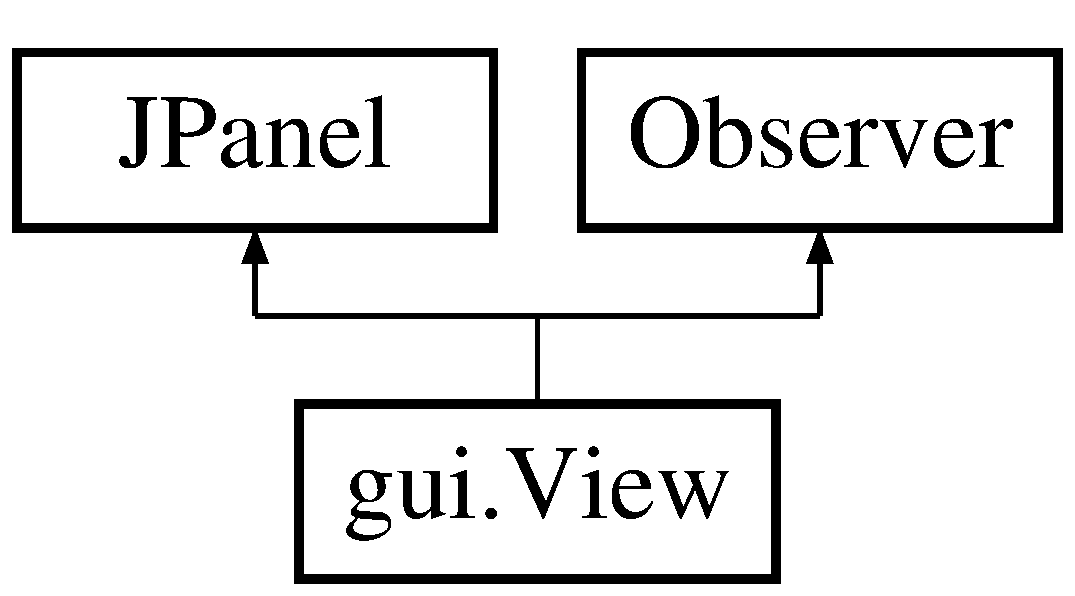
\includegraphics[height=2.000000cm]{classgui_1_1_view}
\end{center}
\end{figure}
\subsection*{Classes}
\begin{DoxyCompactItemize}
\item 
class {\bfseries Board\+Panel}
\item 
class \mbox{\hyperlink{classgui_1_1_view_1_1_score_panel}{Score\+Panel}}
\item 
class \mbox{\hyperlink{classgui_1_1_view_1_1_square_panel}{Square\+Panel}}
\end{DoxyCompactItemize}
\subsection*{Public Member Functions}
\begin{DoxyCompactItemize}
\item 
void \mbox{\hyperlink{classgui_1_1_view_a0b930eff54b741b4a9c9d666180dec00}{update}} (Observable o, Object arg)
\item 
void \mbox{\hyperlink{classgui_1_1_view_af87d7ce351a4529a91bd4cd6215270f3}{add\+Model}} (\mbox{\hyperlink{classgui_1_1_game}{Game}} game)
\item 
void \mbox{\hyperlink{classgui_1_1_view_aa348b4e60405ff1a3948e01b3bc1cf16}{add\+Button\+Controller}} (Action\+Listener button\+Controller)
\item 
void \mbox{\hyperlink{classgui_1_1_view_a66364784fcbb6df611784d77880e98bb}{add\+Piece\+Controller}} (Mouse\+Listener controller)
\item 
Board\+Panel \mbox{\hyperlink{classgui_1_1_view_ad5f7dc8f550cc8895c4da9b5ea8d4b98}{get\+Board\+View}} ()
\item 
Component \mbox{\hyperlink{classgui_1_1_view_aeb332c6eee8b72e856b4eae786e4c736}{get\+Window}} ()
\item 
void \mbox{\hyperlink{classgui_1_1_view_aef80a66972e0010e3ec6b0cd9899bc05}{set\+Has\+Started}} (boolean has\+Started)
\item 
boolean \mbox{\hyperlink{classgui_1_1_view_a958e1dcd8f0a252266b292bff7af26dd}{get\+Has\+Started}} ()
\item 
void \mbox{\hyperlink{classgui_1_1_view_a49679332bb9ef013e497a00188bf254d}{set\+White\+Name}} (String white\+Name)
\item 
void \mbox{\hyperlink{classgui_1_1_view_afe1af467431c5b0f21bf71ef0b869b21}{set\+Black\+Name}} (String black\+Name)
\item 
String \mbox{\hyperlink{classgui_1_1_view_a97fe9c5584520573e63ad4af1988e970}{get\+Black\+Name}} ()
\item 
String \mbox{\hyperlink{classgui_1_1_view_a0c82f77f67a8131b03a10d73cb9e5934}{get\+White\+Name}} ()
\end{DoxyCompactItemize}


\subsection{Member Function Documentation}
\mbox{\Hypertarget{classgui_1_1_view_aa348b4e60405ff1a3948e01b3bc1cf16}\label{classgui_1_1_view_aa348b4e60405ff1a3948e01b3bc1cf16}} 
\index{gui\+::\+View@{gui\+::\+View}!add\+Button\+Controller@{add\+Button\+Controller}}
\index{add\+Button\+Controller@{add\+Button\+Controller}!gui\+::\+View@{gui\+::\+View}}
\subsubsection{\texorpdfstring{add\+Button\+Controller()}{addButtonController()}}
{\footnotesize\ttfamily void gui.\+View.\+add\+Button\+Controller (\begin{DoxyParamCaption}\item[{Action\+Listener}]{button\+Controller }\end{DoxyParamCaption})}

Add controller to buttons and menu items 
\begin{DoxyParams}{Parameters}
{\em button\+Controller} & \\
\hline
\end{DoxyParams}
\mbox{\Hypertarget{classgui_1_1_view_af87d7ce351a4529a91bd4cd6215270f3}\label{classgui_1_1_view_af87d7ce351a4529a91bd4cd6215270f3}} 
\index{gui\+::\+View@{gui\+::\+View}!add\+Model@{add\+Model}}
\index{add\+Model@{add\+Model}!gui\+::\+View@{gui\+::\+View}}
\subsubsection{\texorpdfstring{add\+Model()}{addModel()}}
{\footnotesize\ttfamily void gui.\+View.\+add\+Model (\begin{DoxyParamCaption}\item[{\mbox{\hyperlink{classgui_1_1_game}{Game}}}]{game }\end{DoxyParamCaption})}

Adds the model to the view \mbox{\Hypertarget{classgui_1_1_view_a66364784fcbb6df611784d77880e98bb}\label{classgui_1_1_view_a66364784fcbb6df611784d77880e98bb}} 
\index{gui\+::\+View@{gui\+::\+View}!add\+Piece\+Controller@{add\+Piece\+Controller}}
\index{add\+Piece\+Controller@{add\+Piece\+Controller}!gui\+::\+View@{gui\+::\+View}}
\subsubsection{\texorpdfstring{add\+Piece\+Controller()}{addPieceController()}}
{\footnotesize\ttfamily void gui.\+View.\+add\+Piece\+Controller (\begin{DoxyParamCaption}\item[{Mouse\+Listener}]{controller }\end{DoxyParamCaption})}

Add controller to each square in the board 
\begin{DoxyParams}{Parameters}
{\em controller} & \\
\hline
\end{DoxyParams}
\mbox{\Hypertarget{classgui_1_1_view_a97fe9c5584520573e63ad4af1988e970}\label{classgui_1_1_view_a97fe9c5584520573e63ad4af1988e970}} 
\index{gui\+::\+View@{gui\+::\+View}!get\+Black\+Name@{get\+Black\+Name}}
\index{get\+Black\+Name@{get\+Black\+Name}!gui\+::\+View@{gui\+::\+View}}
\subsubsection{\texorpdfstring{get\+Black\+Name()}{getBlackName()}}
{\footnotesize\ttfamily String gui.\+View.\+get\+Black\+Name (\begin{DoxyParamCaption}{ }\end{DoxyParamCaption})}

Gets the name of the white player \mbox{\Hypertarget{classgui_1_1_view_ad5f7dc8f550cc8895c4da9b5ea8d4b98}\label{classgui_1_1_view_ad5f7dc8f550cc8895c4da9b5ea8d4b98}} 
\index{gui\+::\+View@{gui\+::\+View}!get\+Board\+View@{get\+Board\+View}}
\index{get\+Board\+View@{get\+Board\+View}!gui\+::\+View@{gui\+::\+View}}
\subsubsection{\texorpdfstring{get\+Board\+View()}{getBoardView()}}
{\footnotesize\ttfamily Board\+Panel gui.\+View.\+get\+Board\+View (\begin{DoxyParamCaption}{ }\end{DoxyParamCaption})}

Get the board panel \mbox{\Hypertarget{classgui_1_1_view_a958e1dcd8f0a252266b292bff7af26dd}\label{classgui_1_1_view_a958e1dcd8f0a252266b292bff7af26dd}} 
\index{gui\+::\+View@{gui\+::\+View}!get\+Has\+Started@{get\+Has\+Started}}
\index{get\+Has\+Started@{get\+Has\+Started}!gui\+::\+View@{gui\+::\+View}}
\subsubsection{\texorpdfstring{get\+Has\+Started()}{getHasStarted()}}
{\footnotesize\ttfamily boolean gui.\+View.\+get\+Has\+Started (\begin{DoxyParamCaption}{ }\end{DoxyParamCaption})}

Returns if the game has started \mbox{\Hypertarget{classgui_1_1_view_a0c82f77f67a8131b03a10d73cb9e5934}\label{classgui_1_1_view_a0c82f77f67a8131b03a10d73cb9e5934}} 
\index{gui\+::\+View@{gui\+::\+View}!get\+White\+Name@{get\+White\+Name}}
\index{get\+White\+Name@{get\+White\+Name}!gui\+::\+View@{gui\+::\+View}}
\subsubsection{\texorpdfstring{get\+White\+Name()}{getWhiteName()}}
{\footnotesize\ttfamily String gui.\+View.\+get\+White\+Name (\begin{DoxyParamCaption}{ }\end{DoxyParamCaption})}

Gets the name of the black player \mbox{\Hypertarget{classgui_1_1_view_aeb332c6eee8b72e856b4eae786e4c736}\label{classgui_1_1_view_aeb332c6eee8b72e856b4eae786e4c736}} 
\index{gui\+::\+View@{gui\+::\+View}!get\+Window@{get\+Window}}
\index{get\+Window@{get\+Window}!gui\+::\+View@{gui\+::\+View}}
\subsubsection{\texorpdfstring{get\+Window()}{getWindow()}}
{\footnotesize\ttfamily Component gui.\+View.\+get\+Window (\begin{DoxyParamCaption}{ }\end{DoxyParamCaption})}

Get the J\+Frame \mbox{\Hypertarget{classgui_1_1_view_afe1af467431c5b0f21bf71ef0b869b21}\label{classgui_1_1_view_afe1af467431c5b0f21bf71ef0b869b21}} 
\index{gui\+::\+View@{gui\+::\+View}!set\+Black\+Name@{set\+Black\+Name}}
\index{set\+Black\+Name@{set\+Black\+Name}!gui\+::\+View@{gui\+::\+View}}
\subsubsection{\texorpdfstring{set\+Black\+Name()}{setBlackName()}}
{\footnotesize\ttfamily void gui.\+View.\+set\+Black\+Name (\begin{DoxyParamCaption}\item[{String}]{black\+Name }\end{DoxyParamCaption})}

Sets the name of the black player 
\begin{DoxyParams}{Parameters}
{\em black\+Name} & \\
\hline
\end{DoxyParams}
\mbox{\Hypertarget{classgui_1_1_view_aef80a66972e0010e3ec6b0cd9899bc05}\label{classgui_1_1_view_aef80a66972e0010e3ec6b0cd9899bc05}} 
\index{gui\+::\+View@{gui\+::\+View}!set\+Has\+Started@{set\+Has\+Started}}
\index{set\+Has\+Started@{set\+Has\+Started}!gui\+::\+View@{gui\+::\+View}}
\subsubsection{\texorpdfstring{set\+Has\+Started()}{setHasStarted()}}
{\footnotesize\ttfamily void gui.\+View.\+set\+Has\+Started (\begin{DoxyParamCaption}\item[{boolean}]{has\+Started }\end{DoxyParamCaption})}

set the status which indicate whether the game has started or not 
\begin{DoxyParams}{Parameters}
{\em has\+Started} & the status to update \\
\hline
\end{DoxyParams}
\mbox{\Hypertarget{classgui_1_1_view_a49679332bb9ef013e497a00188bf254d}\label{classgui_1_1_view_a49679332bb9ef013e497a00188bf254d}} 
\index{gui\+::\+View@{gui\+::\+View}!set\+White\+Name@{set\+White\+Name}}
\index{set\+White\+Name@{set\+White\+Name}!gui\+::\+View@{gui\+::\+View}}
\subsubsection{\texorpdfstring{set\+White\+Name()}{setWhiteName()}}
{\footnotesize\ttfamily void gui.\+View.\+set\+White\+Name (\begin{DoxyParamCaption}\item[{String}]{white\+Name }\end{DoxyParamCaption})}

Sets the name of the white player 
\begin{DoxyParams}{Parameters}
{\em white\+Name} & \\
\hline
\end{DoxyParams}
\mbox{\Hypertarget{classgui_1_1_view_a0b930eff54b741b4a9c9d666180dec00}\label{classgui_1_1_view_a0b930eff54b741b4a9c9d666180dec00}} 
\index{gui\+::\+View@{gui\+::\+View}!update@{update}}
\index{update@{update}!gui\+::\+View@{gui\+::\+View}}
\subsubsection{\texorpdfstring{update()}{update()}}
{\footnotesize\ttfamily void gui.\+View.\+update (\begin{DoxyParamCaption}\item[{Observable}]{o,  }\item[{Object}]{arg }\end{DoxyParamCaption})}

Override from Observer, called by the game 

The documentation for this class was generated from the following file\+:\begin{DoxyCompactItemize}
\item 
src/gui/View.\+java\end{DoxyCompactItemize}

\hypertarget{classplayers_1_1_white_player}{}\section{players.\+White\+Player Class Reference}
\label{classplayers_1_1_white_player}\index{players.\+White\+Player@{players.\+White\+Player}}
Inheritance diagram for players.\+White\+Player\+:\begin{figure}[H]
\begin{center}
\leavevmode
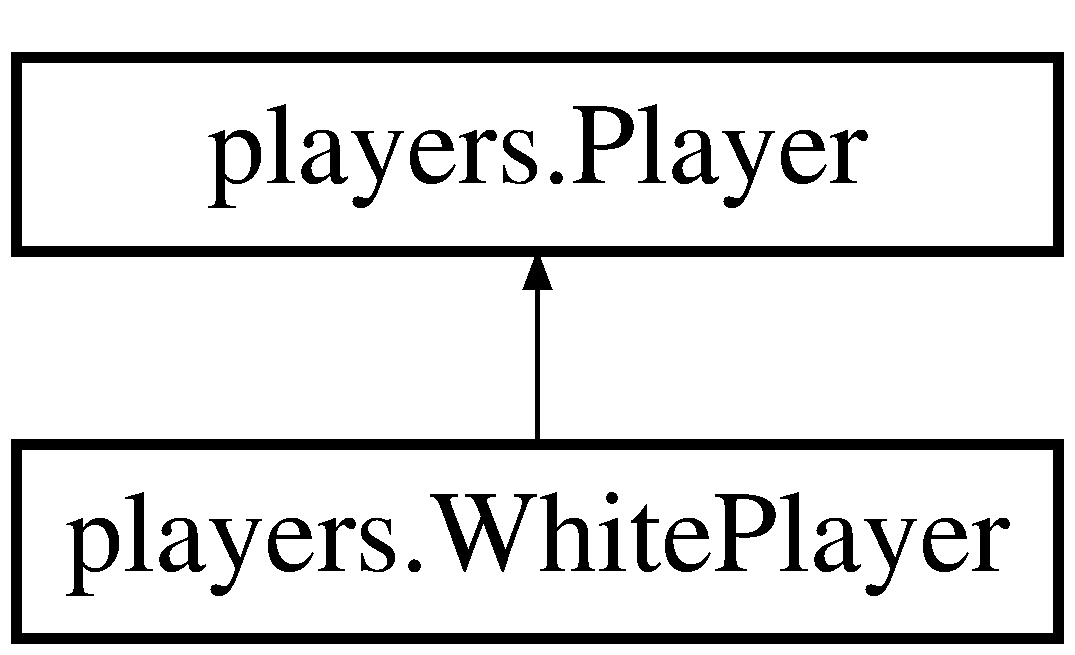
\includegraphics[height=2.000000cm]{classplayers_1_1_white_player}
\end{center}
\end{figure}
\subsection*{Public Member Functions}
\begin{DoxyCompactItemize}
\item 
\mbox{\Hypertarget{classplayers_1_1_white_player_a548112b0d737ce472587a77dc81fd2a5}\label{classplayers_1_1_white_player_a548112b0d737ce472587a77dc81fd2a5}} 
{\bfseries White\+Player} (\mbox{\hyperlink{classgameboard_1_1_game_board}{Game\+Board}} board)
\item 
\mbox{\Hypertarget{classplayers_1_1_white_player_afc74e4fc065579de55c7233fd9b33769}\label{classplayers_1_1_white_player_afc74e4fc065579de55c7233fd9b33769}} 
\mbox{\hyperlink{classpieces_1_1_piece}{Piece}} {\bfseries get\+King} ()
\item 
\mbox{\Hypertarget{classplayers_1_1_white_player_a3dec07e057c5b237cf52afab218fe564}\label{classplayers_1_1_white_player_a3dec07e057c5b237cf52afab218fe564}} 
Set$<$ \mbox{\hyperlink{classpieces_1_1_piece}{Piece}} $>$ {\bfseries get\+Own\+Pieces} ()
\item 
\mbox{\Hypertarget{classplayers_1_1_white_player_aa32d90696bbe466e54ccd60632be1eed}\label{classplayers_1_1_white_player_aa32d90696bbe466e54ccd60632be1eed}} 
Set$<$ \mbox{\hyperlink{classpieces_1_1_piece}{Piece}} $>$ {\bfseries get\+Opponent\+Pieces} ()
\item 
\mbox{\Hypertarget{classplayers_1_1_white_player_a15b686a35a48427a7d76fd33439444ee}\label{classplayers_1_1_white_player_a15b686a35a48427a7d76fd33439444ee}} 
Piece.\+Piece\+Color {\bfseries get\+Color} ()
\end{DoxyCompactItemize}
\subsection*{Additional Inherited Members}


\subsection{Detailed Description}
Represents a player with white pieces Created by Siyang\+Liu on 2018/2/2. 

The documentation for this class was generated from the following file\+:\begin{DoxyCompactItemize}
\item 
src/players/White\+Player.\+java\end{DoxyCompactItemize}

\hypertarget{classtest_1_1_white_player_test}{}\section{test.\+White\+Player\+Test Class Reference}
\label{classtest_1_1_white_player_test}\index{test.\+White\+Player\+Test@{test.\+White\+Player\+Test}}
Inheritance diagram for test.\+White\+Player\+Test\+:\begin{figure}[H]
\begin{center}
\leavevmode
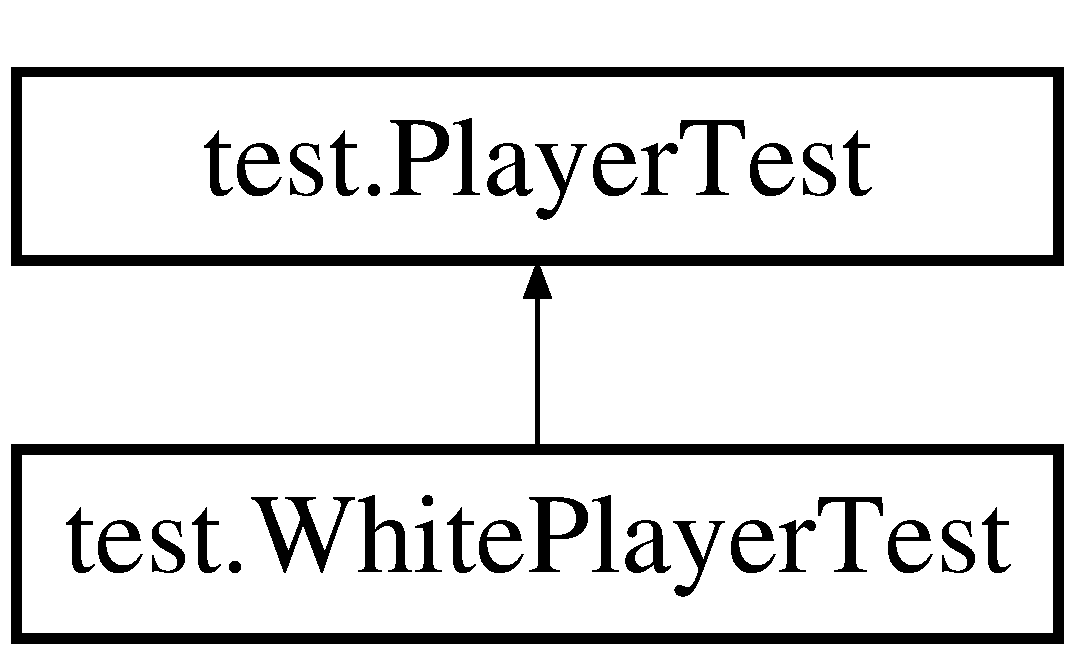
\includegraphics[height=2.000000cm]{classtest_1_1_white_player_test}
\end{center}
\end{figure}
\subsection*{Protected Member Functions}
\begin{DoxyCompactItemize}
\item 
\mbox{\Hypertarget{classtest_1_1_white_player_test_aa42ecc7ee1e37ba91c93278aeb4b56b7}\label{classtest_1_1_white_player_test_aa42ecc7ee1e37ba91c93278aeb4b56b7}} 
\mbox{\hyperlink{classplayers_1_1_player}{Player}} {\bfseries get\+Concrete\+Self} (\mbox{\hyperlink{classgameboard_1_1_game_board}{Game\+Board}} board)
\item 
\mbox{\Hypertarget{classtest_1_1_white_player_test_abbc91632815e5a42f3e2f40094b8a120}\label{classtest_1_1_white_player_test_abbc91632815e5a42f3e2f40094b8a120}} 
\mbox{\hyperlink{classplayers_1_1_player}{Player}} {\bfseries get\+Concrete\+Opponent} (\mbox{\hyperlink{classgameboard_1_1_game_board}{Game\+Board}} board)
\end{DoxyCompactItemize}
\subsection*{Additional Inherited Members}


\subsection{Detailed Description}
Test for the operations of a player with black pieces Created by Siyang\+Liu on 2018/2/4. 

The documentation for this class was generated from the following file\+:\begin{DoxyCompactItemize}
\item 
src/test/White\+Player\+Test.\+java\end{DoxyCompactItemize}

%--- End generated contents ---

% Index
\backmatter
\newpage
\phantomsection
\clearemptydoublepage
\addcontentsline{toc}{chapter}{Index}
\printindex

\end{document}
